%!TEX program = xelatex
%!TEX encoding = UTF-8
%%%%%%%%%%%%%%%%%%%%%%%%%%%%%%%%%%%%%%%%%
% The Legrand Orange Book
% LaTeX Template
% Version 2.3 (8/8/17)
%
% This template has been downloaded from:
% http://www.LaTeXTemplates.com
%
% Original author:
% Mathias Legrand (legrand.mathias@gmail.com) with modifications by:
% Vel (vel@latextemplates.com)
%
% License:
% CC BY-NC-SA 3.0 (http://creativecommons.org/licenses/by-nc-sa/3.0/)

% Compiling this template:
% This template uses biber for its bibliography and makeindex for its index.
% When you first open the template, compile it from the command line with the
% commands below to make sure your LaTeX distribution is configured correctly:
%
% 1) pdflatex main
% 2) makeindex main.idx -s StyleInd.ist
% 3) biber main
% 4) pdflatex main x 2
%
% After this, when you wish to update the bibliography/index use the appropriate
% command above and make sure to compile with pdflatex several times
% afterwards to propagate your changes to the document.
%
% This template also uses a number of packages which may need to be
% updated to the newest versions for the template to compile. It is strongly
% recommended you update your LaTeX distribution if you have any
% compilation errors.
%
% Important note:
% Chapter heading images should have a 2:1 width:height ratio,
% e.g. 920px width and 460px height.
%
%%%%%%%%%%%%%%%%%%%%%%%%%%%%%%%%%%%%%%%%%

\def\ano{2024}
\def\semestre{1}

%----------------------------------------------------------------------------------------
%   PACKAGES AND OTHER DOCUMENT CONFIGURATIONS
%----------------------------------------------------------------------------------------

\documentclass[11pt,fleqn,usenames,dvipsnames]{book} % Default font size and left-justified equations

%----------------------------------------------------------------------------------------

%!TEX program = xelatex
%!TEX root = Algebra_1.tex
%%%%%%%%%%%%%%%%%%%%%%%%%%%%%%%%%%%%%%%%%
% The Legrand Orange Book
% Structural Definitions File
% Version 2.0 (9/2/15)
%
% Original author:
% Mathias Legrand (legrand.mathias@gmail.com) with modifications by:
% Vel (vel@latextemplates.com)
% 
% This file has been downloaded from:
% http://www.LaTeXTemplates.com
%
% License:
% CC BY-NC-SA 3.0 (http://creativecommons.org/licenses/by-nc-sa/3.0/)
%
%%%%%%%%%%%%%%%%%%%%%%%%%%%%%%%%%%%%%%%%%

%----------------------------------------------------------------------------------------
%	VARIOUS REQUIRED PACKAGES AND CONFIGURATIONS
%----------------------------------------------------------------------------------------

\usepackage[top=3cm,bottom=3cm,left=3cm,right=3cm,headsep=10pt,a4paper]{geometry} % Page margins

\usepackage{graphicx} % Required for including pictures
\graphicspath{{Pictures/}} % Specifies the directory where pictures are stored

\usepackage{ccicons} %ícones creative commons

\usepackage{amssymb,amsmath,amsfonts,amsthm,amstext}

\usepackage{enumitem}

\usepackage{lipsum} % Inserts dummy text

\usepackage{tikz} % Required for drawing custom shapes

\usepackage[brazil]{babel}

\usepackage{multicol}

\usepackage{enumitem} % Customize lists
\setlist{nolistsep} % Reduce spacing between bullet points and numbered lists

\usepackage{booktabs} % Required for nicer horizontal rules in tables

\usepackage{xcolor} % Required for specifying colors by name
\definecolor{ocre}{RGB}{243,102,25} % Define the orange color used for highlighting throughout the book

%----------------------------------------------------------------------------------------
%	FONTS
%----------------------------------------------------------------------------------------

\usepackage{avant} % Use the Avantgarde font for headings
%\usepackage{times} % Use the Times font for headings
\usepackage{mathptmx} % Use the Adobe Times Roman as the default text font together with math symbols from the Sym­bol, Chancery and Com­puter Modern fonts

\usepackage{microtype} % Slightly tweak font spacing for aesthetics
\usepackage[utf8]{inputenc} % Required for including letters with accents
\usepackage[T1]{fontenc} % Use 8-bit encoding that has 256 glyphs

%----------------------------------------------------------------------------------------
%	BIBLIOGRAPHY AND INDEX
%----------------------------------------------------------------------------------------

% \usepackage[style=numeric,citestyle=numeric,sorting=nyt,sortcites=true,autopunct=true,babel=hyphen,hyperref=true,abbreviate=false,backref=true,backend=biber]{biblatex}
% \addbibresource{bibliography.bib} % BibTeX bibliography file
% \defbibheading{bibempty}{}

\usepackage{calc} % For simpler calculation - used for spacing the index letter headings correctly
\usepackage{makeidx} % Required to make an index
\makeindex % Tells LaTeX to create the files required for indexing

%----------------------------------------------------------------------------------------
%	MAIN TABLE OF CONTENTS
%----------------------------------------------------------------------------------------

\usepackage{titletoc} % Required for manipulating the table of contents

\contentsmargin{0cm} % Removes the default margin

% Part text styling
\titlecontents{part}[0cm]
{\addvspace{20pt}\centering\large\bfseries}
{}
{}
{}

% Chapter text styling
\titlecontents{chapter}[1.25cm] % Indentation
{\addvspace{12pt}\large\sffamily\bfseries} % Spacing and font options for chapters
{\color{ocre!60}\contentslabel[\Large\thecontentslabel]{1.25cm}\color{ocre}} % Chapter number
{\color{ocre}}  
{\color{ocre!60}\normalsize\;\titlerule*[.5pc]{.}\;\thecontentspage} % Page number

% Section text styling
\titlecontents{section}[1.25cm] % Indentation
{\addvspace{3pt}\sffamily\bfseries} % Spacing and font options for sections
{\contentslabel[\thecontentslabel]{1.25cm}} % Section number
{}
{\hfill\color{black}\thecontentspage} % Page number
[]

% Subsection text styling
\titlecontents{subsection}[1.25cm] % Indentation
{\addvspace{1pt}\sffamily\small} % Spacing and font options for subsections
{\contentslabel[\thecontentslabel]{1.25cm}} % Subsection number
{}
{\ \titlerule*[.5pc]{.}\;\thecontentspage} % Page number
[]

% List of figures
\titlecontents{figure}[0em]
{\addvspace{-5pt}\sffamily}
{\thecontentslabel\hspace*{1em}}
{}
{\ \titlerule*[.5pc]{.}\;\thecontentspage}
[]

% List of tables
\titlecontents{table}[0em]
{\addvspace{-5pt}\sffamily}
{\thecontentslabel\hspace*{1em}}
{}
{\ \titlerule*[.5pc]{.}\;\thecontentspage}
[]

%----------------------------------------------------------------------------------------
%	MINI TABLE OF CONTENTS IN PART HEADS
%----------------------------------------------------------------------------------------

% Chapter text styling
\titlecontents{lchapter}[0em] % Indenting
{\addvspace{15pt}\large\sffamily\bfseries} % Spacing and font options for chapters
{\color{ocre}\contentslabel[\Large\thecontentslabel]{1.25cm}\color{ocre}} % Chapter number
{}  
{\color{ocre}\normalsize\sffamily\bfseries\;\titlerule*[.5pc]{.}\;\thecontentspage} % Page number

% Section text styling
\titlecontents{lsection}[0em] % Indenting
{\sffamily\small} % Spacing and font options for sections
{\contentslabel[\thecontentslabel]{1.25cm}} % Section number
{}
{}

% Subsection text styling
\titlecontents{lsubsection}[.5em] % Indentation
{\normalfont\footnotesize\sffamily} % Font settings
{}
{}
{}

%----------------------------------------------------------------------------------------
%	PAGE HEADERS
%----------------------------------------------------------------------------------------

\usepackage{fancyhdr} % Required for header and footer configuration

\pagestyle{fancy}
\renewcommand{\chaptermark}[1]{\markboth{\sffamily\normalsize\bfseries\chaptername\ \thechapter.\ #1}{}} % Chapter text font settings
\renewcommand{\sectionmark}[1]{\markright{\sffamily\normalsize\thesection\hspace{5pt}#1}{}} % Section text font settings
\fancyhf{} \fancyhead[LE,RO]{\sffamily\normalsize\thepage} % Font setting for the page number in the header
\fancyhead[LO]{\rightmark} % Print the nearest section name on the left side of odd pages
\fancyhead[RE]{\leftmark} % Print the current chapter name on the right side of even pages
\renewcommand{\headrulewidth}{0.5pt} % Width of the rule under the header
\addtolength{\headheight}{2.5pt} % Increase the spacing around the header slightly
\renewcommand{\footrulewidth}{0pt} % Removes the rule in the footer
\fancypagestyle{plain}{\fancyhead{}\renewcommand{\headrulewidth}{0pt}} % Style for when a plain pagestyle is specified

% Removes the header from odd empty pages at the end of chapters
\makeatletter
\renewcommand{\cleardoublepage}{
\clearpage\ifodd\c@page\else
\hbox{}
\vspace*{\fill}
\thispagestyle{empty}
\newpage
\fi}

%----------------------------------------------------------------------------------------
%	THEOREM STYLES
%----------------------------------------------------------------------------------------

\usepackage{amsmath,amsfonts,amssymb,amsthm} % For math equations, theorems, symbols, etc

\newcommand{\intoo}[2]{\mathopen{]}#1\,;#2\mathclose{[}}
\newcommand{\ud}{\mathop{\mathrm{{}d}}\mathopen{}}
\newcommand{\intff}[2]{\mathopen{[}#1\,;#2\mathclose{]}}
\newtheorem{notation}{Notation}[chapter]
\newtheoremstyle{dotless}{}{}{\itshape}{}{\bfseries}{}{ }{}
\theoremstyle{dotless}
\newtheorem*{solucao}{Solu{\c c}{\~a}o:}

% Boxed/framed environments
\newtheoremstyle{ocrenumbox}% % Theorem style name
{0pt}% Space above
{0pt}% Space below
{\normalfont}% % Body font
{}% Indent amount
{\small\bf\sffamily\color{ocre}}% % Theorem head font
{\;}% Punctuation after theorem head
{0.25em}% Space after theorem head
{\small\sffamily\color{ocre}\thmname{#1}\nobreakspace\thmnumber{\@ifnotempty{#1}{}\@upn{#2}}% Theorem text (e.g. Theorem 2.1)
\thmnote{\nobreakspace\the\thm@notefont\sffamily\bfseries\color{black}---\nobreakspace#3.}} % Optional theorem note
\renewcommand{\qedsymbol}{$\blacksquare$}% Optional qed square

\newtheoremstyle{blacknumex}% Theorem style name
{5pt}% Space above
{5pt}% Space below
{\normalfont}% Body font
{} % Indent amount
{\small\bf\sffamily}% Theorem head font
{\;}% Punctuation after theorem head
{0.25em}% Space after theorem head
{\small\sffamily{\tiny\ensuremath{\blacksquare}}\nobreakspace\thmname{#1}\nobreakspace\thmnumber{\@ifnotempty{#1}{}\@upn{#2}}% Theorem text (e.g. Theorem 2.1)
\thmnote{\nobreakspace\the\thm@notefont\sffamily\bfseries---\nobreakspace#3.}}% Optional theorem note

\newtheoremstyle{blacknumbox} % Theorem style name
{0pt}% Space above
{0pt}% Space below
{\normalfont}% Body font
{}% Indent amount
{\small\bf\sffamily}% Theorem head font
{\;}% Punctuation after theorem head
{0.25em}% Space after theorem head
{\small\sffamily\thmname{#1}\nobreakspace\thmnumber{\@ifnotempty{#1}{}\@upn{#2}}% Theorem text (e.g. Theorem 2.1)
\thmnote{\nobreakspace\the\thm@notefont\sffamily\bfseries---\nobreakspace#3.}}% Optional theorem note

% Non-boxed/non-framed environments
\newtheoremstyle{ocrenum}% % Theorem style name
{5pt}% Space above
{5pt}% Space below
{\normalfont}% % Body font
{}% Indent amount
{\small\bf\sffamily\color{ocre}}% % Theorem head font
{\;}% Punctuation after theorem head
{0.25em}% Space after theorem head
{\small\sffamily\color{ocre}\thmname{#1}\nobreakspace\thmnumber{\@ifnotempty{#1}{}\@upn{#2}}% Theorem text (e.g. Theorem 2.1)
\thmnote{\nobreakspace\the\thm@notefont\sffamily\bfseries\color{black}---\nobreakspace#3.}} % Optional theorem note
\renewcommand{\qedsymbol}{$\blacksquare$}% Optional qed square
\makeatother

% Defines the theorem text style for each type of theorem to one of the three styles above
\newcounter{dummy} 
\numberwithin{dummy}{section}
\theoremstyle{ocrenumbox}
\newtheorem{teoremaT}[dummy]{Teorema}
\newtheorem{problema}{Problema}[chapter]
\newtheorem{exercicio}{Exercício}[chapter]
\theoremstyle{blacknumex}
\newtheorem{exemplo}{Exemplo}[chapter]
\newtheorem{exemplos}{Exemplos}[chapter]
\newtheorem{observacao}{Observaçao}[chapter]
\newtheorem{observacoes}{Observações}[chapter]
\newtheorem{nota}{Nota}[chapter]
\theoremstyle{blacknumbox}
\newtheorem{vocabulary}{Vocabulary}[chapter]
\newtheorem{definicaoT}{Definição}[section]
\newtheorem{definicoesT}{Definições}[section]
\newtheorem{corolarioT}[dummy]{Corolário}
\theoremstyle{ocrenum}
\newtheorem{proposicao}[dummy]{Proposição}
\newenvironment{prova}[1][Prova]{\noindent\textbf{#1:} }{\qedsymbol}%{\ \rule{0.5em}{0.5em}}

%----------------------------------------------------------------------------------------
%	MATH COMMANDS
%----------------------------------------------------------------------------------------


\newcommand{\n}{\mathbb{N}}
\newcommand{\z}{\mathbb{Z}}
\newcommand{\rac}{\mathbb{Q}}
\newcommand{\dom}{{\rm dom\,}}
\newcommand{\im}{{\rm Im\,}}
\newcommand{\aut}{{\rm Aut\,}}
\newcommand{\cp}[1]{\mathbb{#1}}
\newcommand{\sub}{\subseteq}
\newcommand{\real}{\mathbb{R}}
\newcommand{\complex}{\mathbb{C}}
\newcommand{\lap}[1]{\mathcal{L}\left\{#1\right\}}
\newcommand{\lapi}[1]{\mathcal{L}^{-1}\left\{#1\right\}}
\newcommand{\se}[1]{\displaystyle\sum_{n = 1}^\infty{#1}}
\newcommand{\dlim}[2]{\displaystyle\lim_{#1\rightarrow #2}}
\newcommand{\slim}{\displaystyle\lim_{n \rightarrow \infty}}
\newcommand{\seq}[1]{\{{#1_n\}}}
\newcommand{\seg}[1]{\displaystyle\sum_{n = 1}^\infty{#1_n}}
\newcommand{\sei}[2]{\displaystyle\sum_{#1}^\infty{#2}}
\newcommand{\sepc}[3]{\displaystyle\sum_{#1}^\infty{#2(x - #3)^n}}
\newcommand{\imp}[3]{\displaystyle\int_{#1}^{+\infty}{#3}{d #2}}
\newcommand{\dint}[4]{\displaystyle\int_{#1}^{#2}{#4}{d#3}}
\newcommand{\inti}[2]{\displaystyle\int{#1}{d#2}}
\newcommand{\norma}[1]{\left\lVert#1\right\rVert}
\newcommand{\flim}[1]{\displaystyle\lim_{#1\rightarrow \infty}}
\renewcommand{\sin}{{\rm sen\,}}
\renewcommand{\tan}{{\rm tg\,}}
\renewcommand{\csc}{{\rm cossec\,}}
\renewcommand{\cot}{{\rm cotg\,}}
\renewcommand{\sinh}{{\rm senh\,}}
\newcommand\T{\rule{0pt}{2.6ex}} 


%----------------------------------------------------------------------------------------
%	DEFINITION OF COLORED BOXES
%----------------------------------------------------------------------------------------

\RequirePackage[framemethod=default]{mdframed} % Required for creating the theorem, definition, exercise and corollary boxes

% Theorem box
\newmdenv[skipabove=7pt,
skipbelow=7pt,
backgroundcolor=black!5,
linecolor=ocre,
innerleftmargin=5pt,
innerrightmargin=5pt,
innertopmargin=5pt,
leftmargin=0cm,
rightmargin=0cm,
innerbottommargin=5pt]{tBox}

% Exercise box	  
\newmdenv[skipabove=7pt,
skipbelow=7pt,
rightline=false,
leftline=true,
topline=false,
bottomline=false,
backgroundcolor=ocre!10,
linecolor=ocre,
innerleftmargin=5pt,
innerrightmargin=5pt,
innertopmargin=5pt,
innerbottommargin=5pt,
leftmargin=0cm,
rightmargin=0cm,
linewidth=4pt]{eBox}	

% Definition box
\newmdenv[skipabove=7pt,
skipbelow=7pt,
rightline=false,
leftline=true,
topline=false,
bottomline=false,
linecolor=ocre,
innerleftmargin=5pt,
innerrightmargin=5pt,
innertopmargin=0pt,
leftmargin=0cm,
rightmargin=0cm,
linewidth=4pt,
innerbottommargin=0pt]{dBox}	

% Corollary box
\newmdenv[skipabove=7pt,
skipbelow=7pt,
rightline=false,
leftline=true,
topline=false,
bottomline=false,
linecolor=gray,
backgroundcolor=black!5,
innerleftmargin=5pt,
innerrightmargin=5pt,
innertopmargin=5pt,
leftmargin=0cm,
rightmargin=0cm,
linewidth=4pt,
innerbottommargin=5pt]{cBox}

% Creates an environment for each type of theorem and assigns it a theorem text style from the "Theorem Styles" section above and a colored box from above
\newenvironment{teorema}{\begin{tBox}\begin{teoremaT}}{\end{teoremaT}\end{tBox}}
\newenvironment{exercise}{\begin{eBox}\begin{exerciseT}}{\hfill{\color{ocre}\tiny\ensuremath{\blacksquare}}\end{exerciseT}\end{eBox}}				  
\newenvironment{definicao}{\begin{dBox}\begin{definicaoT}}{\end{definicaoT}\end{dBox}}	
\newenvironment{definicoes}{\begin{dBox}\begin{definicoesT}}{\end{definicoesT}\end{dBox}}	
\newenvironment{example}{\begin{exampleT}}{\hfill{\tiny\ensuremath{\blacksquare}}\end{exampleT}}		
\newenvironment{corolario}{\begin{cBox}\begin{corolarioT}}{\end{corolarioT}\end{cBox}}	

%----------------------------------------------------------------------------------------
%	REMARK ENVIRONMENT
%----------------------------------------------------------------------------------------

\newenvironment{remark}{\par\vspace{10pt}\small % Vertical white space above the remark and smaller font size
\begin{list}{}{
\leftmargin=35pt % Indentation on the left
\rightmargin=25pt}\item\ignorespaces % Indentation on the right
\makebox[-2.5pt]{\begin{tikzpicture}[overlay]
\node[draw=ocre!60,line width=1pt,circle,fill=ocre!25,font=\sffamily\bfseries,inner sep=2pt,outer sep=0pt] at (-15pt,0pt){\textcolor{ocre}{R}};\end{tikzpicture}} % Orange R in a circle
\advance\baselineskip -1pt}{\end{list}\vskip5pt} % Tighter line spacing and white space after remark


\newenvironment{remarks}{\par\vspace{10pt}\small % Vertical white space above the remark and smaller font size
\begin{list}{}{
\leftmargin=35pt % Indentation on the left
\rightmargin=25pt}\item\ignorespaces % Indentation on the right
\makebox[-2.5pt]{\begin{tikzpicture}[overlay]
\node[draw=ocre!60,line width=1pt,circle,fill=ocre!25,font=\sffamily\bfseries,inner sep=2pt,outer sep=0pt] at (-15pt,0pt){\textcolor{ocre}{R}};\end{tikzpicture}} % Orange R in a circle
\advance\baselineskip -1pt}{\end{list}\vskip5pt} % Tighter line spacing and white space after remark

%----------------------------------------------------------------------------------------
%	SECTION NUMBERING IN THE MARGIN
%----------------------------------------------------------------------------------------

\makeatletter
\renewcommand{\@seccntformat}[1]{\llap{\textcolor{ocre}{\csname the#1\endcsname}\hspace{1em}}}                    
\renewcommand{\section}{\@startsection{section}{1}{\z@}
{-4ex \@plus -1ex \@minus -.4ex}
{1ex \@plus.2ex }
{\normalfont\large\sffamily\bfseries}}
\renewcommand{\subsection}{\@startsection {subsection}{2}{\z@}
{-3ex \@plus -0.1ex \@minus -.4ex}
{0.5ex \@plus.2ex }
{\normalfont\sffamily\bfseries}}
\renewcommand{\subsubsection}{\@startsection {subsubsection}{3}{\z@}
{-2ex \@plus -0.1ex \@minus -.2ex}
{.2ex \@plus.2ex }
{\normalfont\small\sffamily\bfseries}}                        
\renewcommand\paragraph{\@startsection{paragraph}{4}{\z@}
{-2ex \@plus-.2ex \@minus .2ex}
{.1ex}
{\normalfont\small\sffamily\bfseries}}

%----------------------------------------------------------------------------------------
%	PART HEADINGS
%----------------------------------------------------------------------------------------

% numbered part in the table of contents
\newcommand{\@mypartnumtocformat}[2]{%
\setlength\fboxsep{0pt}%
\noindent\colorbox{ocre!20}{\strut\parbox[c][.7cm]{\ecart}{\color{ocre!70}\Large\sffamily\bfseries\centering#1}}\hskip\esp\colorbox{ocre!40}{\strut\parbox[c][.7cm]{\linewidth-\ecart-\esp}{\Large\sffamily\centering#2}}}%
%%%%%%%%%%%%%%%%%%%%%%%%%%%%%%%%%%
% unnumbered part in the table of contents
\newcommand{\@myparttocformat}[1]{%
\setlength\fboxsep{0pt}%
\noindent\colorbox{ocre!40}{\strut\parbox[c][.7cm]{\linewidth}{\Large\sffamily\centering#1}}}%
%%%%%%%%%%%%%%%%%%%%%%%%%%%%%%%%%%
\newlength\esp
\setlength\esp{4pt}
\newlength\ecart
\setlength\ecart{1.2cm-\esp}
\newcommand{\thepartimage}{}%
\newcommand{\partimage}[1]{\renewcommand{\thepartimage}{#1}}%
\def\@part[#1]#2{%
\ifnum \c@secnumdepth >-2\relax%
\refstepcounter{part}%
\addcontentsline{toc}{part}{\texorpdfstring{\protect\@mypartnumtocformat{\thepart}{#1}}{\partname~\thepart\ ---\ #1}}
\else%
\addcontentsline{toc}{part}{\texorpdfstring{\protect\@myparttocformat{#1}}{#1}}%
\fi%
\startcontents%
\markboth{}{}%
{\thispagestyle{empty}%
\begin{tikzpicture}[remember picture,overlay]%
\node at (current page.north west){\begin{tikzpicture}[remember picture,overlay]%	
\fill[ocre!20](0cm,0cm) rectangle (\paperwidth,-\paperheight);
\node[anchor=north] at (4cm,-3.25cm){\color{ocre!40}\fontsize{220}{100}\sffamily\bfseries\thepart}; 
\node[anchor=south east] at (\paperwidth-1cm,-\paperheight+1cm){\parbox[t][][t]{8.5cm}{
\printcontents{l}{0}{\setcounter{tocdepth}{1}}%
}};
\node[anchor=north east] at (\paperwidth-1.5cm,-3.25cm){\parbox[t][][t]{15cm}{\strut\raggedleft\color{white}\fontsize{30}{30}\sffamily\bfseries#2}};
\end{tikzpicture}};
\end{tikzpicture}}%
\@endpart}
\def\@spart#1{%
\startcontents%
\phantomsection
{\thispagestyle{empty}%
\begin{tikzpicture}[remember picture,overlay]%
\node at (current page.north west){\begin{tikzpicture}[remember picture,overlay]%	
\fill[ocre!20](0cm,0cm) rectangle (\paperwidth,-\paperheight);
\node[anchor=north east] at (\paperwidth-1.5cm,-3.25cm){\parbox[t][][t]{15cm}{\strut\raggedleft\color{white}\fontsize{30}{30}\sffamily\bfseries#1}};
\end{tikzpicture}};
\end{tikzpicture}}
\addcontentsline{toc}{part}{\texorpdfstring{%
\setlength\fboxsep{0pt}%
\noindent\protect\colorbox{ocre!40}{\strut\protect\parbox[c][.7cm]{\linewidth}{\Large\sffamily\protect\centering #1\quad\mbox{}}}}{#1}}%
\@endpart}
\def\@endpart{\vfil\newpage
\if@twoside
\if@openright
\null
\thispagestyle{empty}%
\newpage
\fi
\fi
\if@tempswa
\twocolumn
\fi}

%----------------------------------------------------------------------------------------
%	CHAPTER HEADINGS
%----------------------------------------------------------------------------------------

% A switch to conditionally include a picture, implemented by  Christian Hupfer
\newif\ifusechapterimage
\usechapterimagetrue
\newcommand{\thechapterimage}{}%
\newcommand{\chapterimage}[1]{\ifusechapterimage\renewcommand{\thechapterimage}{#1}\fi}%
\newcommand{\autodot}{.}
\def\@makechapterhead#1{%
{\parindent \z@ \raggedright \normalfont
\ifnum \c@secnumdepth >\m@ne
\if@mainmatter
\begin{tikzpicture}[remember picture,overlay]
\node at (current page.north west)
{\begin{tikzpicture}[remember picture,overlay]
\node[anchor=north west,inner sep=0pt] at (0,0) {\ifusechapterimage\includegraphics[width=\paperwidth]{\thechapterimage}\fi};
\draw[anchor=west] (\Gm@lmargin,-9cm) node [line width=2pt,rounded corners=15pt,draw=ocre,fill=white,fill opacity=0.5,inner sep=15pt]{\strut\makebox[22cm]{}};
\draw[anchor=west] (\Gm@lmargin+.3cm,-9cm) node {\huge\sffamily\bfseries\color{black}\thechapter\autodot~#1\strut};
\end{tikzpicture}};
\end{tikzpicture}
\else
\begin{tikzpicture}[remember picture,overlay]
\node at (current page.north west)
{\begin{tikzpicture}[remember picture,overlay]
\node[anchor=north west,inner sep=0pt] at (0,0) {\ifusechapterimage\includegraphics[width=\paperwidth]{\thechapterimage}\fi};
\draw[anchor=west] (\Gm@lmargin,-9cm) node [line width=2pt,rounded corners=15pt,draw=ocre,fill=white,fill opacity=0.5,inner sep=15pt]{\strut\makebox[22cm]{}};
\draw[anchor=west] (\Gm@lmargin+.3cm,-9cm) node {\huge\sffamily\bfseries\color{black}#1\strut};
\end{tikzpicture}};
\end{tikzpicture}
\fi\fi\par\vspace*{270\p@}}}

%-------------------------------------------

\def\@makeschapterhead#1{%
\begin{tikzpicture}[remember picture,overlay]
\node at (current page.north west)
{\begin{tikzpicture}[remember picture,overlay]
\node[anchor=north west,inner sep=0pt] at (0,0) {\ifusechapterimage\includegraphics[width=\paperwidth]{\thechapterimage}\fi};
\draw[anchor=west] (\Gm@lmargin,-9cm) node [line width=2pt,rounded corners=15pt,draw=ocre,fill=white,fill opacity=0.5,inner sep=15pt]{\strut\makebox[22cm]{}};
\draw[anchor=west] (\Gm@lmargin+.3cm,-9cm) node {\huge\sffamily\bfseries\color{black}#1\strut};
\end{tikzpicture}};
\end{tikzpicture}
\par\vspace*{270\p@}}
\makeatother

%----------------------------------------------------------------------------------------
%	HYPERLINKS IN THE DOCUMENTS
%----------------------------------------------------------------------------------------

\usepackage{hyperref}
\hypersetup{hidelinks,backref=true,pagebackref=true,hyperindex=true,colorlinks=false,breaklinks=true,urlcolor= ocre,bookmarks=true,bookmarksopen=false,pdftitle={Title},pdfauthor={Author}}
\usepackage{bookmark}
\bookmarksetup{
open,
numbered,
addtohook={%
\ifnum\bookmarkget{level}=0 % chapter
\bookmarksetup{bold}%
\fi
\ifnum\bookmarkget{level}=-1 % part
\bookmarksetup{color=ocre,bold}%
\fi
}
}
 % Insert the commands.tex file which contains the majority of the structure behind the template

\tikzset{
     >=stealth,
    bullet/.style={
      fill=black,
      circle,
      minimum width=1pt,
      inner sep=1pt
    }
}
\begin{document}

%----------------------------------------------------------------------------------------
%   TITLE PAGE
%----------------------------------------------------------------------------------------

\begingroup
\thispagestyle{empty}
\begin{tikzpicture}[remember picture,overlay]
\node[inner sep=0pt] (background) at (current page.center) {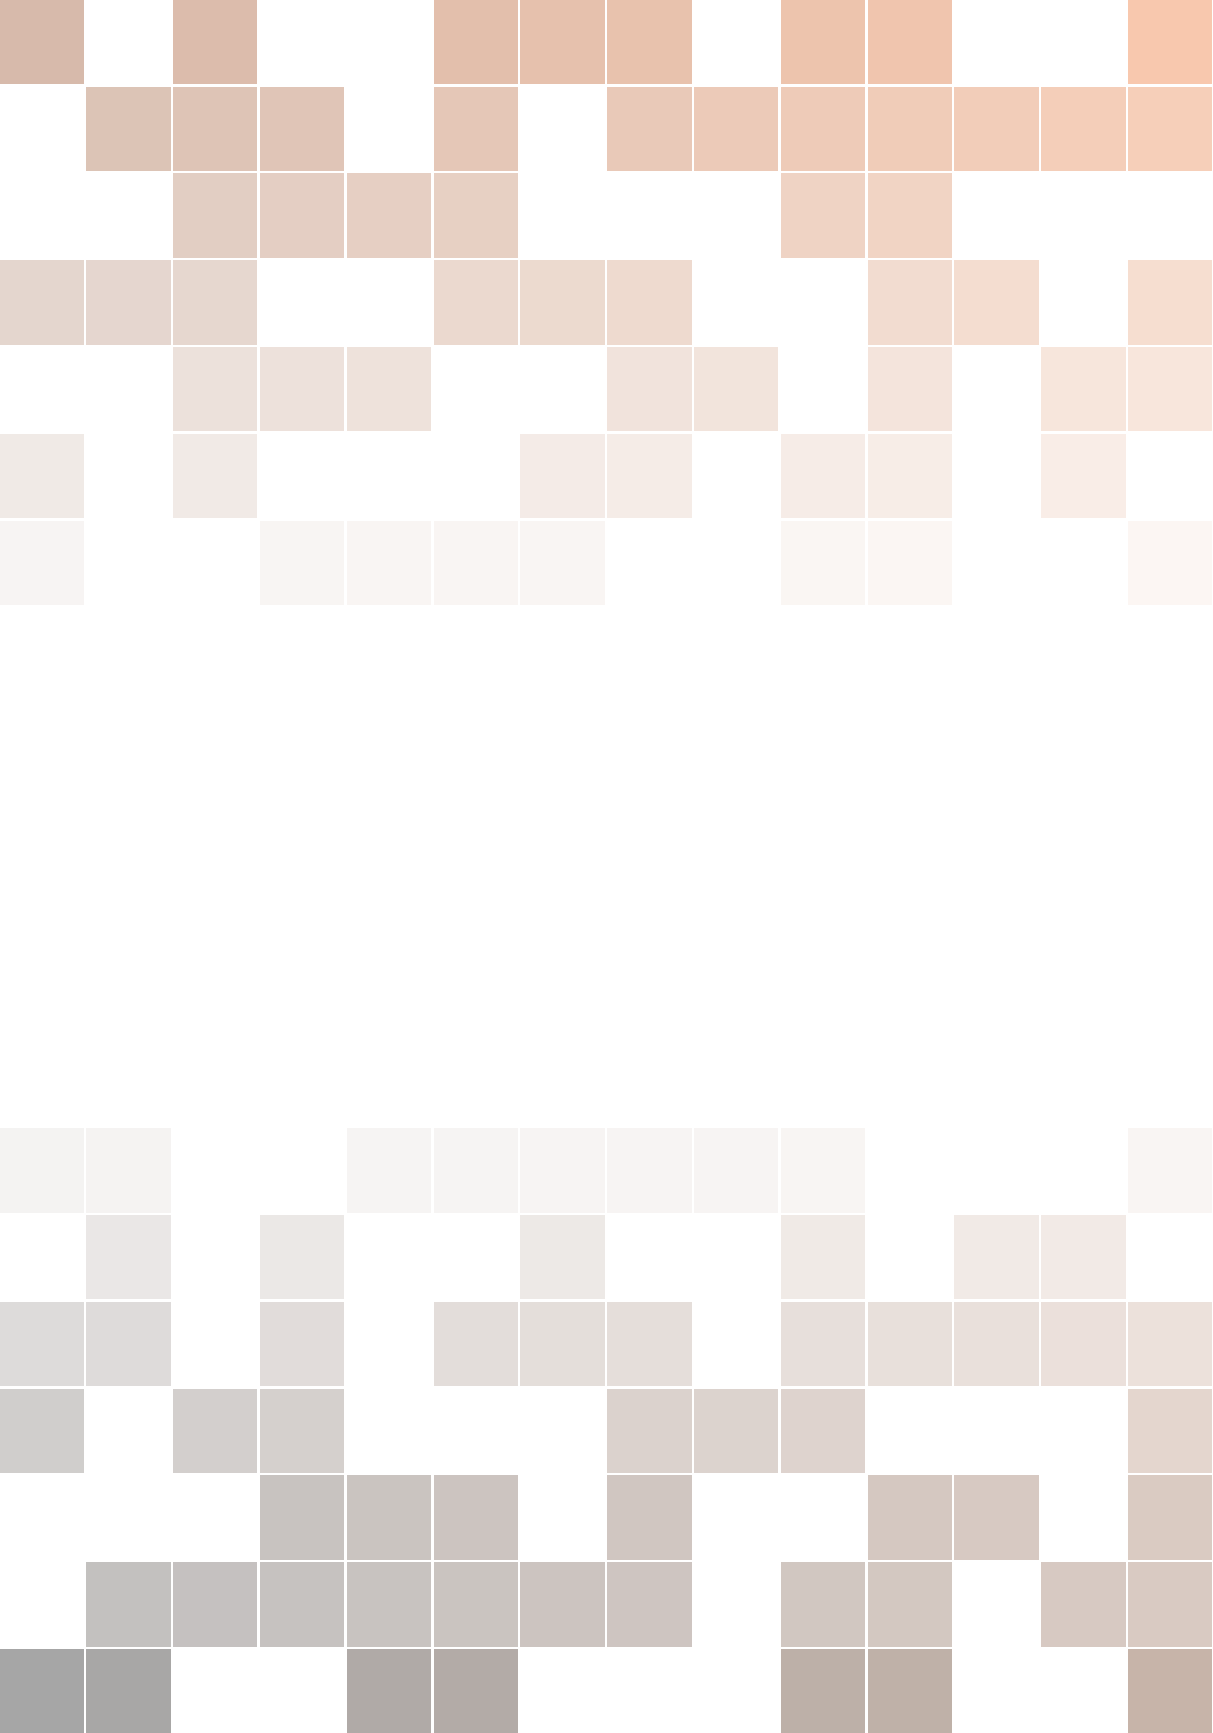
\includegraphics[width=\paperwidth]{background}};
\draw (current page.center) node [fill=ocre!30!white,fill opacity=0.6,text opacity=1,inner sep=1cm]{\Huge\centering\bfseries\sffamily\parbox[c][][t]{\paperwidth}{\centering Álgebra 1\\[15pt] % Book title
{\Large Notas de Aula \semestre/\ano}\\[20pt] % Subtitle
{\huge José Antônio O. Freitas}\\
{\large \today}}}; % Author name

\end{tikzpicture}
\vfill
\endgroup

%----------------------------------------------------------------------------------------
%   COPYRIGHT PAGE
%----------------------------------------------------------------------------------------

\newpage
~\vfill
\thispagestyle{empty}

\noindent \ccbyncsa\ Este texto está licenciado sob uma \textbf{Licença Creative Commons Atribuição-NãoComercial-CompartilhaIgual 3.0 Brasil} \href{http://creativecommons.org/licenses/by-nc-sa/3.0/br/deed.pt\_BR}{\textit{http://creativecommons.org/licenses/by-nc-sa/3.0/br/deed.pt\_BR}}\\ % Copyright notice

%----------------------------------------------------------------------------------------
%   TABLE OF CONTENTS
%----------------------------------------------------------------------------------------

\usechapterimagefalse % If you don't want to include a chapter image, use this to toggle images off - it can be enabled later with \usechapterimagetrue

\chapterimage{chapter_head_1.pdf} % Table of contents heading image

\pagestyle{empty} % No headers

\tableofcontents % Print the table of contents itself

\cleardoublepage % Forces the first chapter to start on an odd page so it's on the right

\pagestyle{fancy} % Print headers again

%!TEX program = xelatex
%!TEX root = Algebra_1.tex
%%Usar makeindex -s indexstyle.ist arquivo.idx no terminal para gerar o í}ndice remissivo agrupado por inicial
%%Após executar pdflatex arquivo
\begin{center}
\Huge \textbf{Prefácio}
\end{center}

Essas notas de Aula são referentes à matéria Álgebra 1,
ministrada na UnB - Universidade de Brasília - durante o 2$^o$ Semestre de 2010
pelo professor José Antônio O. de Freitas, Departamento de Matemática. Tais
notas foram transcritas e editadas pelo graduando em Ciências Econômicas
Luiz Eduardo Sol R. da Silva\footnote{luizeduardosol@hotmail.com}.

Revisão e ampliação das notas feita por José Antônio O. de Freitas\footnote{jfreitas@mat.unb.br}.


É livre a reprodução, distribuição e edição deste material, desde que citadas as suas fontes e autores. Críticas e sugestões são bem vindas.
\vspace{20cm}




% \begin{center} \textbf{\Large Notações e expressões}
% \end{center}
% \begin{minipage}[l]{0,5\textwidth}
% \begin{itemize}
% \item $\neg$ Não
% \item $\forall$ Para todo
% \item $/$ Tal que
% \item $|$ Divide
% \item $\Rightarrow$ Implica
% \item $\in$ Pertence
% \item $\emptyset$ Vazio
% \item $\subseteq$ Contido ou igual a
% \item $\supseteq$ Contém ou igual a
% \item $\wedge$ E
% \item $\vee$ Ou
% \item $=$ Igual
% \item $\neq$ Diferente
% \item $\mathbb{Z}$ N{\'u}meros Inteiros
% \item $\mathbb{R}$ N{\'u}meros Reais
% \item $\cap$ Intersecção
% \item $>$ Maior que
% \item $\geq$ Maior ou igual a
% \item $\displaystyle\bigcup_{i=1}^{n}$ União de $n$ conjuntos
% \item $\displaystyle\bigsqcup_{i=1}^{n}$ União disjunta de $n$ conjuntos


% \end{itemize}
% \end{minipage}
% \begin{minipage}[r]{0,5\textwidth}
% \begin{itemize}

% \item $\leftrightarrow$ Se, e somente se
% \item $\veebar$ Ou...,ou..., mas nunca ambos
% \item $\rightarrow$ Se,... então...
% \item $\exists$ Existe
% \item $\Leftrightarrow$ Equivalente a
% \item $\notin$ Não pertence
% \item \# Fim da demonstração
% \item $\mathbb{N}$ N{\'u}meros Naturais
% \item $\mathbb{Q}$ N{\'u}meros Racionais
% \item $\nsubseteq$ Não contém ou é igual a
% \item $\cup$ União
% \item $\sqcup$ União Disjunta
% \item $<$ Menor que
% \item $\leq$ Menor ou igual a
% \item $\displaystyle\bigcap_{i=1}^{n}$ Intersecção de $n$ conjuntos
% \item Q.E.D. (\textit{Quod Erat Demonstrandum}): Como se queria demonstrar
% \item P.B.O.: Princí}pio da boa ordenação
% \item H.I.: Hip{ó}tese de Indução
% \item \textit{Mutatis Mutandis}:  Mudando o que tem que ser mudado

% \end{itemize}
% \end{minipage}
%!TEX program = xelatex
%!TEX root = Algebra_1.tex
%!TEX encoding = UTF-8
%%Usar makeindex -s indexstyle.ist arquivo.idx no terminal para gerar o índice remissivo agrupado por inicial
%%Após executar pdflatex arquivo
\chapter{Conceitos Básicos} % (fold)
\label{cha:conceitos_basicos}

\begin{definicao}
    Uma \textbf{proposição} é todo conjunto de palavras ou símbolos ao qual podemos atribuir um \textbf{valor lógico}.
\end{definicao}

\begin{definicao}
    Diz-se que o \textbf{valor lógico} de uma proposição é ``verdade'' (V) se a proposição é verdadeira ou ``falsidade'' (F) se a proposição é falsa.
\end{definicao}

\begin{exemplos}
    Julgue se as seguintes sentenças são ou não proposições:
    \begin{enumerate}[label={\arabic*})]
        \item Todo número primo é ímpar.
        \begin{solucao}
            Essa sentença é uma proposição de valor lógico "Falsidade."
        \end{solucao}

        \item $x^2 + y^2 \ge 0$ para todos $x$, $y \in \real$.
        \begin{solucao}
            Esse sentença é uma proposição de valor lógico "Verdade".
        \end{solucao}

        \item Amanhã irá chover.
        \begin{solucao}
            Essa sentença não é uma proposição. Não é possível atribuir um valor lógico a ela.
        \end{solucao}
    \end{enumerate}

\end{exemplos}

\section{Princípio da não contradição e do terceiro excluído} % (fold)
\label{sec:principio_da_nao_contradicao_e_do_3}
\begin{enumerate}[label={\roman*})]
    \item Uma proposição não pode ser verdadeira e falsa ao mesmo tempo.
    \item Toda proposição ou é verdadeira ou é falsa, isto é, verifica-se sempre um destes casos e nunca um terceiro.
\end{enumerate}

Assim esses princípios afirmam que:
\begin{center}
    ``Toda proposição tem um, e um só, dos valores lógicos \textbf{verdade} ou \textbf{falsidade}.''
\end{center}

De modo geral vamos trabalhar com proposições da forma:
\begin{enumerate}[label={\roman*})]
    \item Se $\mathbb{H}$, então $\mathbb{T}$.

    Aqui $\mathbb{H}$ é chamado de hipótese e $\mathbb{T}$ de tese. Neste tipo de proposição iremos admitir que $\mathbb{H}$ é uma verdade e precisaremos provar que $\mathbb{T}$ é verdade. Ou seja precisamos construir um argumento que justifique $\mathbb{T}$ ser verdadeira à partir do fato de $\mathbb{H}$ ser verdadeira.

    \item $\mathbb{H}$ se, e somente se, $\mathbb{T}$ ou $\mathbb{H}$ se, e só se, $\mathbb{T}$.

    Esse tipo de proposição será decomposta em duas proposições no formato anterior. Isto é:
    \begin{enumerate}[label={\alph*})]
        \item Se $\mathbb{H}$, então $\mathbb{T}$.
        \item Se $\mathbb{T}$, então $\mathbb{H}$.
    \end{enumerate}

    No primeiro caso admitimos $\mathbb{H}$ verdadeira e provamos que $\mathbb{T}$ também é verdadeira e no segundo caso admitimos que $\mathbb{T}$ é verdadeira e provamos que $\mathbb{H}$ é verdadeira.
\end{enumerate}

Para demonstrarmos uma proposição precisamos deduzí-la de proposições previamente comprovadas como verdadeiras. Assim uma demonstração é a determinação de uma verdade e é construída através de uma sequência de raciocínios lógicos, com início e fim determinados. Cada passo dessa sequência de raciocínio deve ter sua veracidade justificada, seja através de outras proposições já provadas verdadeiras ou pelo uso de axiomas, que são afirmações admitidas como verdadeiras. Vamos utilizar, principalmente, três formas de demonstrar uma proposição, a saber:
\begin{enumerate}[label={\roman*})]
    \item Demonstração direta;
    \item Demonstração por contraposição;
    \item Demonstração por contradição ou redução ao absurdo.
\end{enumerate}

Assim numa proposição do tipo:
\begin{center}
    Se $\mathbb{H}$, então $\mathbb{T}$.
\end{center}

Para demonstrá-la de forma \textbf{direta} devemos admitir que a hipótese $\mathbb{H}$ é \textbf{verdadeira} e, utilizando de uma sequência de passos
cuja veracidade podemos comprovar, chegar à conclusão que a tese $\mathbb{T}$ também é \textbf{verdadeira}.

Na \textbf{demonstração por contraposição}, iremos supor que a tese $\mathbb{T}$ é \textbf{falsa} e novamente através de uma
sequência de passos que podemos justificar como verdadeiros, devemos chegar à conclusão que a hipótese $\mathbb{H}$ também é
\textbf{falsa}. Se conseguirmos chegar a essa conclusão então a proposição original será \textbf{verdadeira}.

Por último, na \textbf{demonstração por contradição} ou \textbf{redução ao absurdo}, iremos admitir que a hipótese
$\mathbb{H}$ é \textbf{verdadeira} e que a tese $\mathbb{T}$ é \textbf{falsa}. Usando essas suposições devemos chegar à alguma
conclusão contraditória, isto é, precisamos obter alguma informação que seja verdadeira e falsa ao mesmo tempo. Nesse caso,
significa que nossa tese $\mathbb{T}$ deve ser obrigatoriamente \textbf{verdadeira}, e com isso a proposição também será
\textbf{verdadeira}.

% section príncipio_da_não_contradição_e_do_3 (end)

% chapter conceitos_básicos (end)

\chapter{Noções de Teoria de Conjuntos}
\section{Conceitos básicos}

Um conjunto é uma ``coleção'' ou ``família'' de elementos.

Usaremos letras maiúsculas do alfabeto para denotar os conjuntos e denotaremos elementos de um dado conjunto por letras minúsculas do alfabeto.

Dado um conjunto $A$, para indicar o fato de que $x$ é um elemento de $A$, escrevemos:
\[
    x \in A.
\]

Para dizer que um elemento $x$ não pertence ao conjunto $A$, escrevemos:
\[
    x \notin A.
\]

Um conjunto sem elementos é chamado de \textbf{conjunto vazio}. Tal conjunto é denotado por $\emptyset$ ou por $\{\ \}$.

Dado um conjunto $A$ e $x$ um elemento, ocorre sempre uma das seguintes situações:
\[
    x \in A \mbox{ ou } x \notin A.
\]

Além disso, para dois elementos $x$, $y \in A$, ocorre exatamente uma das seguinte situações:
\[
    x = y \mbox{ ou } x \neq y.
\]

\section{Descrição de um conjunto}

Um conjunto $A$ pode ser dado pela simples listagem dos seus elementos, como por exemplo:
\begin{align*}
    A &= \{1,2,3,4,5\}\\
    B &= \{verdadeiro, falso\}.
\end{align*}

Um conjunto também pode ser dado pela descrição das propriedades dos seus elementos, como por exemplo:
\[
    A = \{\mbox{números naturais\ } n \mid n \mbox{ é múltiplo de } 2\} = \{2,4,6,...\}.
\]

\section{Alguns conjuntos importantes}
\begin{enumerate}[label={\arabic*})]
    \item $\n = \{0,1,2,3,...\}$ o conjunto dos números naturais.
    \item $\n^* = \{1,2,3,...\}$ o conjunto dos números naturais estritamente maiores que zero.
    \item $\z = \{...,-2,-1,0,1,2,...\}$ o conjunto dos números inteiros.
    \item $\rac = \left\{\dfrac{p}{q} \mid p,q \in \z, q \neq 0 \right\}$ o conjunto dos números racionais.
    \item $\real $ o conjunto dos números reais.
    \item $\real^*$ o conjunto dos números reais não nulos.
    \item $\complex = \{a + bi \mid a,b \in \real,\ i^2 = -1\}$ o conjunto dos números complexos.
\end{enumerate}

\begin{observacao}
    Para esses conjuntos vamos admitir como verdadeiras as propriedades básicas da soma e multiplicação.
\end{observacao}
\section{Propriedades dos conjuntos}

\begin{definicao}\label{igualdade_conjuntos}
    Dados dois conjuntos $A$ e $B$, dizemos que $A$ e $B$ são \textbf{iguais} se, e somente se, eles têm os mesmos elementos. Ou seja, para todo $x \in A$ também vale que $x \in B$ e para todo $y \in B$ também vale que $y \in A$. Se $A$ e $B$ são iguais, escrevemos $A = B$.
\end{definicao}

\begin{exemplo}
    Sejam $A = \{1,1,2,3,4,4\}$, $B = \{3,2,1,4\}$, $C = \{1,2,3\}$ e $D = \{2,3\}$. Então de acordo com a Definição
    \ref{igualdade_conjuntos} temos $A = B$ pois todo elemento de $A$ está em $B$ e todo elemento de $B$ também está em $A$. Agora
    como $1 \in C$ e $1 \notin D$, então $C \ne D$.
\end{exemplo}

\begin{observacao}
    Dados conjuntos $A$ e $B$, de acordo com a Definição \ref{igualdade_conjuntos} para que $A \ne B$ basta que exista um elemento $x \in A$ de maneira que $x \notin B$ ou que exista $y \in B$ com a condição de que $y \notin A$.
\end{observacao}

\begin{definicao}\label{definicao_continencia_conjuntos}
    Se $A$ e $B$ são dois conjuntos, dizemos que $A$ é um \textbf{subconjunto} de $B$ ou que $A$ \textbf{está contido} em $B$ ou que $B$ \textbf{contém} $A$ se todo elemento de $A$ for elemento de $B$. Ou seja, se para todo elemento $x \in A$, temos $x \in B$. Nesse caso, escrevemos $A \subseteq B$ (ou $A \subset B$) ou $B \supseteq A$ (ou $B \supset A$).
\end{definicao}


Caso $A$ seja um subconjunto de $B$ mas não é igual a $B$, escrevemos:
\[
    A \subsetneq B.
\]

Nesse caso, dizemos que $A$ é um \textbf{subconjunto pr{ó}prio} de $B$.

\begin{exemplos}
    Sejam $A = \{1,2,3,x,y,z\}$, $B = \{x, y\}$ e $C = \{x, y , z\}$. Temos:
    \begin{enumerate}[label={\arabic*})]
        \item $A \nsubseteq B$ pois $1 \in A$ e $1 \notin B$.
        \item $B \subsetneq A$ pois todo elemento de $B$ também está em $A$. Observe que existem elementos de $A$ que não estão em $B$, por exemplo $2 \in A$ e $2 \notin B$.
        \item $B \subseteq C$ pois todo elemento de $B$ também está em $C$.
        \item $C \subseteq A$ pois todo elemento de $C$ também está em $A$.
    \end{enumerate}
\end{exemplos}

\begin{observacao}
    Dados dois conjuntos $A$ e $B$ pela Definição \ref{definicao_continencia_conjuntos} para que $A$ \textbf{não esteja contido em} $B$ basta que exista $x \in A$ tal que $x \notin B$. Nesse caso escrevemos $A \nsubseteq B$.
\end{observacao}

Usando a definição de continência de conjuntos, Definição \ref{definicao_continencia_conjuntos}, podemos redefinir a igualdade de conjuntos, Definição \ref{igualdade_conjuntos}, da seguinte forma: dados dois conjuntos $A$ e $B$
\begin{center}
    $A = B$\quad \textbf{se, e somente se,}\quad $A \subseteq B$\quad \textbf{e}\quad $B \subseteq A$.
\end{center}

Ou seja,
\begin{center}
    \textbf{se} $A = B$ \textbf{então} $A \subseteq B$ \textbf{e} $B \subseteq A$.
\end{center}

Além disso,
\begin{center}
    \textbf{se} $A \subseteq B$ \textbf{e} $B \subseteq A$, \textbf{então} $A = B$.
\end{center}

Quando $A$ e $B$ não são iguais, escrevemos $A \neq B$. Para que $A \neq B$ devemos ter $A \nsubseteq B$ ou $B \nsubseteq A$. Isto é, precisamos encontrar algum elemento $x \in A$ de modo que $x \notin B$ ou então encontrar $y \in B$ com a condição de que $y \notin A$.

\begin{proposicao}
    Dados três conjuntos $A$, $B$ e $C$ temos:
    \begin{enumerate}[label={\roman*})]
        \item $A\subseteq A$ (Reflexividade)
        \item Se $A\subseteq B \mbox{ e } B\subseteq A$, então $A=B$. (Antissimetria)
        \item Se $A\subseteq B$ e $B\subseteq C$, então $A\subseteq C$. (Transitividade)
    \end{enumerate}
\end{proposicao}


Considere os seguintes conjuntos:
\begin{align*}
    A &= \{ n \in \n \mid n \mbox{ é múltiplo de } 2\} = \{2,4,6,...\}\\
    B &= \{n \in \n \mid n \mbox{ é múltiplo de } 3\} = \{3,6,9,...\}.
\end{align*}


Neste caso, $2 \in A$ e $2 \notin B$, logo $A \nsubseteq B$. Por outro lado, $3 \in B$ e $3 \notin A$ e com isso $B \nsubseteq A$. Portanto, dados dois conjuntos $A$ e $B$, nem sempre temos $A \subseteq B$ ou $B \subseteq A$.

\begin{proposicao}
    Seja $A$ um conjunto. Então $ \emptyset \subseteq A$.
\end{proposicao}
\begin{prova}
    Suponha que $\emptyset \nsubseteq A$. Logo existe $x \in \emptyset$ tal que $x \notin A$. Mas por definição, o conjunto vazio não contém elementos. Logo a existência de $x \in \emptyset$ é uma contradição. Tal contradição surgiu por termos suposto que $\emptyset \nsubseteq A$. Portanto, $\emptyset \subseteq A$, como queríamos demonstrar.
\end{prova}

\section{Relações entre conjuntos}

\begin{definicao}\label{intersecao_conjunto}
    Sejam $A$ e $B$ dois conjuntos. Definimos a \textbf{intersecção} de $A$ e $B$ como sendo o conjunto $A \cap B$ cujos elementos pertencem aos conjuntos $A$ e $B$ simultaneamente. Assim,
    \[
        A \cap B = \{x \mid x \in A\mbox{ e }  x \in B\}.
    \]

    \begin{tikzpicture}[thick,
    set/.style = {circle,
        minimum size = 3cm,
        fill=MidnightBlue!50}]

% Set A
\node[set,label={135:$A$}] (A) at (0,0) {};

% Set B
\node[set,label={45:$B$}] (B) at (1.8,0) {};

% Intersection
\begin{scope}
    \clip (0,0) circle(1.5cm);
    \clip (1.8,0) circle(1.5cm);
    \fill[Dandelion](0,0) circle(1.5cm);
\end{scope}

% Circles outline
\draw (0,0) circle(1.5cm);
\draw (1.8,0) circle(1.5cm);

% Set intersection label
\node at (0.9,0) {$A\cap B$};

\end{tikzpicture}
\end{definicao}

\begin{exemplo}
    Sejam $A = \{1, 2, 3\}$, $B = \{2, 3, 4\}$ e $C = \{r, s, t\}$. Então
    \begin{align*}
        A \cap B &= \{2, 3\}\\
        A \cap C &= \emptyset.
    \end{align*}
\end{exemplo}

\begin{definicao}\label{unicao_conjuntos}
    Sejam $A$ e $B$ dois conjuntos. Definimos a \textbf{união} de $A$ com $B$ como sendo o conjunto $A \cup B$, cujos elementos pertencem ao conjunto $A$ ou ao conjunto $B$. Assim,
    \[
        A \cup B = \{x \mid x \in A \mbox{ ou } x \in B\}.
    \]

    \begin{tikzpicture}[thick,set/.style = {circle,fill=orange,minimum size =3cm}]

        % Set A
        \node [set,label={135:$A$}] (A) at (0,0){};

        % Set B
        \node [set,label={45:$B$}] (B) at (1.8,0){};

        % Circles outline
        \draw[white] (0,0) circle(1.5cm);
        \draw[white] (1.8,0) circle(1.5cm);

        % Union text label
        \node[orange!90!black] at (0.9,1.8) {$A\cup B$};

    \end{tikzpicture}
\end{definicao}

\begin{exemplo}
    Sejam $A = \{1, 2, 3\}$, $B = \{2, 3, 4\}$ e $C = \{r, s, t\}$. Então
    \begin{align*}
        A \cup B &= \{1,2,3,4\}\\
        A \cup C &= \{1,2,3,r,s,t\}.
    \end{align*}
\end{exemplo}

\begin{proposicao} Sejam $A$ e $B$ dois conjuntos. Então:
    \begin{enumerate}[label={\roman*})]
        \item $(A \cap B) \subseteq A$;
        \item $(A \cap B) \subseteq B$;
        \item $A \subseteq A \cup B$;
        \item $B \subseteq A \cup B$.
    \end{enumerate}
\end{proposicao}
\begin{prova}
    Para provar a primeira afirmação seja $x \in A \cap B$ um elemento qualquer. Da definição de interseção de conjuntos, Definição \ref{intersecao_conjunto}, temos $x \in A$ e $x \in B$. Assim podemos afirmar com certeza que $x \in A$. Logo todo elemente de $A \cap B$ também está em $A$, ou seja, $A \cap B \subseteq A$. De modo análogo prova-se a segunda afirmação sobre a interseção.

    Para a terceira afirmação, seja $x \in A$. Da definição de união de conjuntos, Definição \ref{unicao_conjuntos}, segue que $x \in A \cup B$. Logo todo elemento de $A$ também está em $A \cup B$, ou seja, $A \subseteq (A \cup B)$. De modo análogo prova-se a quarta afirmação.
\end{prova}

O conceito de união ($ \cup $) e intersecção ($ \cap $) pode ser estendido para mais de dois conjuntos.

\begin{definicao}
    Sejam $A_{1}$, $A_2$, \dots, $A_{n}$ conjuntos. Então
    \[
        A_{1} \cup A_{2} \cup \cdots \cup A_{n}= \displaystyle\bigcup_{k=1}^n A_{k}
    \]
    é o conjunto dos elementos $x$ tais que $x$ pertence a pelo menos um dos conjuntos $A_{1}$, $A_2$, \dots, $A_{n}$. Agora,
    \[
        A_{1} \cap A_2 \cap \cdots \cap A_{n} = \displaystyle\bigcap_{k=1}^{n}A_{k}
    \]
    é o conjunto dos elementos $x$ que pertencem a todos os conjuntos $A_{1}$, $A_2$, \dots, $A_{n}$ simultaneamente.
\end{definicao}

\begin{definicao}
    Sejam $A$ e $B$ conjuntos. Se $A \cap B = \emptyset$, dizemos que $A$ e $B$ são \textbf{conjuntos disjuntos}.
\end{definicao}


Sejam $A$ e $B$ conjuntos tais que $C = A \cup B$ e $A \cap B = \emptyset$. Neste caso dizemos que $C$ é uma \textbf{união disjunta} de $A$ e $B$. Denotamos tal fato por
\[
    C = A \sqcup B.
\]

\begin{proposicao} Sejam $A,\ B$ e $C$ três conjuntos, então:
    \begin{enumerate}[label={\roman*})]
        \item $A \cap (B \cup C) = (A \cap B) \cup (A \cap C)$
        \item $A \cup (B \cap C) = (A \cup B) \cap (A \cup C)$.
    \end{enumerate}
\end{proposicao}
\begin{prova}
    \begin{enumerate}[label={\roman*})]
        \item Precisamos mostrar que
        \begin{enumerate}[label=({\arabic*})]
            \item $A\cap(B\cup C)\subseteq(A\cap B)\cup(A\cap C)$;\label{intersecao_unicao_1}
            \item $(A\cap B)\cup(A\cap C)\subseteq A\cap(B\cup C).$\label{intersecao_unicao_2}
        \end{enumerate}

        Para provar \ref{intersecao_unicao_1} seja $x\in A \cap (B \cup C)$. Logo $x\in A$ e $x\in B\cup C$. Agora, de $x\in B\cup C$, segue que $x\in B$ ou $x\in C$. Suponha que $x\in B$. Como $x\in A$ e $x \in B$, então $x\in A\cap B$. Assim, $x\in(A\cap B)\cup(A\cap C)$, ou seja, $A\cap(B\cup C)\subseteq(A\cap B)\cup(A\cap C)$. Por outro lado, se $x\in C$, como $x\in A$, então $x\in A\cap C$ e daí $x\in(A\cap B)\cup(A\cap C)$, logo $A\cap(B\cup C)\subseteq(A\cap B)\cup(A\cap C)$.

        Portanto,
        \[
            A\cap(B\cup C)\subseteq(A\cap B)\cup(A\cap C).
        \]

        Agora para provar \ref{intersecao_unicao_2}, seja $x\in(A\cap B)\cup(A\cap C)$. Daí, $x\in A\cap B$ ou $x\in A\cap C$. Suponha que $x\in A\cap B$. Assim, $x\in A$ e $x\in B$. Como $x\in B$, segue que $x\in B\cup C$ e então $x\in A\cap(B\cup C)$, ou seja, $(A\cap B)\cup(A\cap C)\subseteq A\cap(B\cup C)$. Agora, suponha que $x\in A\cap C$. Com isso $x\in A$ e $x\in C$. Desse modo, $x\in B\cup C$ e então $x\in A\cap(B\cup C)$ e daí
        \[
            (A\cap B)\cup(A\cap C)\subseteq A\cap(B\cup C).
        \]

        Portanto
        \[
            A\cap(B\cup C)=(A\cap B)\cup(A\cap C),
        \]
        como queríamos.
        \item Análoga ao caso anterior.
    \end{enumerate}
\end{prova}

\begin{definicao}
    Dados dois conjuntos $A$ e $B$, definimos a \textbf{diferença} dos conjuntos $A$ e $B$, denotada por $A-B$ ou $A\backslash B$ como sendo o conjunto
    \[
        A - B = \{x \mid x \in A \mbox{ e } x \notin B\}.
    \]

    \begin{tikzpicture}[thick,set/.style = { circle, minimum size = 3cm}]

        % Set A
        \node[set,fill=OliveGreen,label={135:$A$}] (A) at (0,0) {};

        % Set B
        \node[set,fill=white,label={45:$B$}] (B) at (0:2) {};

        % Circles outline
        \draw (0,0) circle(1.5cm);
        \draw (2,0) circle(1.5cm);

        % Difference text label
        \node[left,white] at (A.center){$A-B$};

    \end{tikzpicture}
\end{definicao}

\begin{exemplos}
    \begin{enumerate}[label={\arabic*})]
        \item Se $A=\{1,2,3,5,4\}$, $B=\{2,3,6,8\}$, então
        \begin{align*}
            A - B &= \{1,4,5\}\\
            B - A &=\{6,8\}.
        \end{align*}
        \item Se $A=\{2,4,6,8,10,...\}$, $B=\{3,6,9,12,15,...\}$, então
        \begin{align*}
             A - B &= \{2,4,8,10,14,16,...\}\\
             B - A &= \{3,9,15,21,...\}
         \end{align*}
    \end{enumerate}

\end{exemplos}

\begin{proposicao}
    Sejam $A$, $B$ e $C$ conjuntos não vazios. Então
    \[
        (A \cup B) - C = (A - C) \cup (B - C).
    \]
\end{proposicao}
\begin{prova}
    Precisamos mostrar que
    \begin{enumerate}[label={\arabic*})]
        \item $(A \cup B) - C \sub (A - C) \cup (B - C)$
        \item $(B - C) \sub (A \cup B) - C = (A - C)$
    \end{enumerate}
    Para a primeira inclusão seja $x \in (A \cup B) - C$. Assim por definição, $x \in A \cup B$ e $x \notin C$. De $x \in A \cup B$, então $x \in A$ ou $x \in B$.

    Se $x \in A$, como $x \notin C$ segue então que $x \in A - C$. Logo $x \in (A - C) \cup (B - C)$.

    Se $x \in B$, como $x \notin C$ segue então que $x \in B - C$. Logo $x \in (A - C) \cup (B - C)$.

    Assim $(A \cup B) - C = (A - C) \sub (B - C)$.

    Agora, para a segunda inclusão, seja $y \in (A - C) \cup (B - C)$. Por definição, $x \in A - C$ ou $x \in B - C$.

    Se $x \in A - C$, então $x \in A$ e $x \notin C$. Como $x \in A$, segue que $x \in A \cup B$. Mas $x \notin C$, com isso, $x \in (A \cup B) - C$.

    Se $x \in B - C$, então $x \in B$ e $x \notin C$. Como $x \in B$, segue que $x \in A \cup B$. Mas $x \notin C$, com isso, $x \in (A \cup B) - C$.
    Assim $(A - B) \cup (B - C) \sub (A \cup B) - C$.

    Portanto, $(A \cup B) - C = (A - C) \cup (B - C)$, como queríamos.
\end{prova}

\begin{definicao}
    Dados dois conjuntos $A$ e $E$ tais que $A\subseteq E$, definimos o \textbf{complementar} de $A$ em $E$, denotado $A^C$ ou $C_E(A)$, como
    \[
        C_E(A) = \{ x \in E \mid x \notin A \}.
    \]

    \begin{tikzpicture}
        \fill[Green!55!white, even odd rule](5,-2) rectangle (-2,2) (0:2cm);
        \fill[white] (1.5, 0) circle[radius=1.5];
        \draw[black] (1.5, 0) circle [radius=1.5];

        \node at (1.5, 0) (A) {$A$};
        \node at (4, 1) (C) {$C_E(A)$};
        \node at (5, 2.2) (E) {$E$};
    \end{tikzpicture}
\end{definicao}

\begin{observacoes}
    \begin{enumerate}[label={\arabic*})]
        \item Se $A = E$, então $C_A(A) = \{ x \in A \mid x \notin A \} = \emptyset$.
        \item $(A^C)^C = \{x \in E \mid x \notin A^C\} = \{ x \in E \mid x \in A \} = A$
    \end{enumerate}

\end{observacoes}

\begin{exemplo}
    Sejam $A = \{1,2,3,4\}$ e $E = \{1,2,3,5,4,0,8,9\}$. Primeiro note que $A \subseteq E$, daí
    \[
            A^C = C_E(A) = \{0,5,8,9\}.
    \]
\end{exemplo}

\begin{proposicao}
    Sejam $A$, $B$ e $E$ conjuntos. Se $A\subseteq B\subseteq E$, então $C_E(B)\subseteq C_E(A)$.
\end{proposicao}
\begin{prova}
    Seja $x \in C_E(B)$. Assim $x\notin B$ e como $A \subseteq B$, então $x \notin A$. Daí por definição $x\in C_E(A)$, ou seja, $C_E(B) \subseteq C_E(A)$.
\end{prova}

\begin{proposicao} Sejam $A$, $B$ e $E$ três conjuntos tais que $A\subseteq E$ e $B\subseteq E$. Então:
\begin{enumerate}[label={\roman*})]
    \item $(A\cup B)^C = A^C\cap B^C$
    \item $(A\cap B)^C = A^C\cup B^C$
\end{enumerate}
\end{proposicao}
\begin{prova}
    \begin{enumerate}[label={\roman*})]
        \item Seja $x \in (A\cup B)^C$. Logo $x\notin A\cup B$, assim $x\notin A$ e $x\notin B$. Daí, $x\in A^C$ e $x\in B^C$, isto é, $x\in A^C\cap B^C$. Desse modo,
        \begin{equation}\label{complementar_uniao-1}
            (A\cup B)^C \subseteq A^C\cap B^C.
        \end{equation}

        Por outro lado, se $x\in A^C\cap B^C$, então $x\in A^C$ e $x\in B^C$. Com isso, $x\notin A$ e $x\notin B$, ou seja, $x\notin A\cup B$, logo $x\in (A\cup B)^C$. Desse modo
        \begin{equation}\label{complementar_uniao-2}
            A^C\cap B^C\subseteq(A\cup B)^C.
        \end{equation}

        Portanto, de \eqref{complementar_uniao-1} e \eqref{complementar_uniao-2} temos
        \[
            (A\cup B)^C = A^C\cap B^C.
        \]

        \item Seja $x \in (A\cap B)^C$. Logo $x\notin A\cap B$, assim $x\notin A$ ou $x\notin B$. Então $x\in A^C$ ou $x\in B^C$, isto é, $x\in A^C\cup B^C$. Desse modo,
        \begin{equation}\label{complementar_intersecao-1}
            (A\cap B)^C \subseteq A^C\cup B^C.
        \end{equation}

        Por outro lado, se $x\in A^C\cup B^C$, então $x\in A^C$ ou $x\in B^C$. Daí, $x\notin A$ ou $x\notin B$, ou seja, $x\notin A\cap B$, logo $x\in (A\cap B)^C$. Desse modo
        \begin{equation}\label{complementar_intersecao-2}
            A^C\cup B^C\subseteq(A\cap B)^C.
        \end{equation}

        Portanto, de \eqref{complementar_intersecao-1} e \eqref{complementar_intersecao-2} temos
        \[
            (A\cap B)^C = A^C\cup B^C.
        \]
    \end{enumerate}
\end{prova}

\begin{definicao}
    Dados dois conjuntos $A$ e $B$, definimos o \textbf{produto cartesiano} de $A$ por $B$ como sendo o conjunto
    \[
        A \times B = \{(x,y) \mid x\in A, y\in B\}.
    \]
\end{definicao}

Dados $(x,y)$, $(z,t) \in A\times B$, temos
\begin{center}
    $(x,y) = (z,t)$ \textbf{se, e somente se,} $x = z$ \textbf{e} $y = t$.
\end{center}

\begin{exemplo}\label{exemplo_produto_cartesiano}
    Sejam $A = \{1,2\}$ e $B = \{3,4\}$. Então
    \begin{align*}
        A \times B &= \{(1,3), (1,4), (2,3), (2,4)\}\\
        B \times A &= \{(3,1), (3,2), (4,1), (4,2)\}
\end{align*}
\end{exemplo}

\begin{observacoes}
    \begin{enumerate}[label={\arabic*})]
        \item Do Exemplo \eqref{exemplo_produto_cartesiano} vemos que em geral $A \times B \neq B\times A$.
        \item No caso em que $A = B$ vamos escrever
        \[
            A \times A = A^2 = \{ (x, y) \mid x, y \in A\}.
        \]
        De modo geral:
        \[
            \underbrace{A \times A \times \cdots \times A}_{n\ vezes} = A^n = \{ (x_1, x_2, \dots, x_n) \mid x_1, x_2, \dots, x_n \in A\}
        \]
        para $n \ge 2$.
    \end{enumerate}
\end{observacoes}

\begin{definicao}
    Para qualquer conjunto $A$, indicamos por $\mathcal{P}(A)$ o conjunto
    \[
        \mathcal{P}(A) = \{ X \mid X\subseteq A\}
    \]
    que é chamado de \textbf{conjunto das partes} de $A$.
\end{definicao}

Os elementos desse conjunto são todos os subconjuntos de $A$. Dizer que $Y\in \mathcal{P}(A)$ significa que $Y \subseteq A$. Particularmente, temos $\emptyset\in \mathcal{P}(A)$ e $A\in \mathcal{P}(A)$.

\begin{exemplos}
    \begin{enumerate}[label={\arabic*})]
        \item $A = \emptyset$, $\mathcal{P}(A) = \{\emptyset\}$;
        \item $B = \{x\}$, $\mathcal{P}(B) = \{\emptyset, \{x\}\}$;
        \item $C = \{a,b,c\}$, $\mathcal{P}(C)=\{\emptyset, \{a\}, \{b\},\{c\},\{a,b\},\{a,c\},\{b,c\},C\}$;
        \item $D=\real$, $\mathcal{P}(D)=\{X\mid X \subseteq \real\}$, por exemplo $\rac\in \mathcal{P}(D)$.
    \end{enumerate}
\end{exemplos}

%!TEX program = xelatex
%!TEX root = Algebra_1.tex
%%Usar makeindex -s indexstyle.ist arquivo.idx no terminal para gerar o índice remissivo agrupado por inicial
%%Após executar pdflatex arquivo
% \chapter{Relações e Funções}
\chapter{Relações}
% \section{Relações}
% \subsubsection{Definição}
% Sejam A e B dois conjuntos não vazios. Os subconjuntos de AxB são chamados relações, ou seja, uma relação em AxB é um subconjunto desse produto cartesiano.

% Quando $R$ é uma relação em $A \times B$, também dizemos que $R$ é uma relação de A em B.

% Exemplos:
% \begin{enumerate}[label={\arabic*})]
% \item Se A=\{0,1\} e B=\{-1,0,1\}, então AxB=\{(0,-1),(0,0),(0,1),(1,-1),(1,0),(1,1,)\}\\
% São exemplos de relações:\\
% $R_{1}=\{(0,1)\}$\\
% $R_{2}=\emptyset$\\
% $R_{3}=\{(1,-1),(1,1)\}$\\
% $R_{4}=A$x$B$
% \item Se $A=B=\mathbb{R}$, então AxB é o conjunto formado por todos pares ordenados de números reais. Um exemplo de relação em $\mathbb{R}$x$\mathbb{R}$ é o conjunto:\\
% $R=\{(x,y)\in \mathbb{R}$x$\mathbb{R}/ y\geq 0\}$
% \end{enumerate}

\section{Relações de equivalência}

\begin{definicao}\label{definicao_relacao_equivalencia}
    Seja $A$ um conjunto não vazio e $R\subseteq A \times A$. Dizemos que $R$ é uma \textbf{relação de equivalência} se:
    \begin{enumerate}[label={\roman*})]
        \item Para todo $x \in A$, $(x,x) \in R$. \textit{(Propriedade Reflexiva)}
        \item Se $(x, y) \in R$, então $(y, x) \in R$. \textit{(Propriedade Simétrica)}
        \item Se $(x, y) \in R$ e $(y, z) \in R$, então $(x, z)\in R$. \textit{(Propriedade Transitiva)}
    \end{enumerate}
\end{definicao}

Quando $R\subseteq A \times A$ é uma relação de equivalência, dizemos que $R$ é uma relação de equivalência em $A$. Quando dois elementos $x$, $y \in A$ são tais que $(x,y) \in R$, dizemos que $x$ e $y$ \textbf{são relacionados} ou que $x$ e $y$ \textbf{estão relacionados}.

\begin{exemplos}\label{exemplos_relacoes_equivalencia}
    \begin{enumerate}[label={\arabic*})]
        \item Seja A=\{1,2,3,4\}. Temos
        \begin{align*}
            A\times A = &\{(1,1);(1,2);(1,3);(1,4);(2,1);(2,2);(2,3);(2,4);\\ &(3,1);(3,2);(3,3);(3,4);(4,1);(4,2);(4,3);(4,4)\}.
        \end{align*}
        Quais dos seguintes conjuntos são exemplos de relações de equivalência?
        \begin{itemize}
            \item $R_{1}= A\times A$
            \item $R_{2}=\{(1,1);(2,2);(3,3)\}$
            \item $R_{3}=\{(1,1);(2,2);(3,3);(4,4);(1,2);(2,1)\}$
            \item $R_{4}=\{(1,1);(2,2);(3,3);(4,4)\}$
            \item $R_{5}=\{(1,1);(2,2);(3,3);(4,4);(1,2);(2,1);(2,4);(4;2)\}$
        \end{itemize}
        \begin{solucao}
            $R_2$ não é relação de equivalência pois $(4,4) \notin R_2$.

            $R_5$ não é relação de equivalência pois, por exemplo, $(1,4) \notin R_5$.

            Os demais são exemplos de relações de equivalência.
        \end{solucao}

        \item Seja $A = \z$ e $R\subseteq \z\times \z$ definida por $R = \{(x,y)\in \z \times \z \mid x = y\}$.
        Então $R$ é uma relação de equivalência.
        \begin{solucao}
            De fato,
            \begin{itemize}
                \item Para todo $x \in \z$ temos $x = x$ daí $(x,x) \in R$.
                \item Se $(x,y)\in R$, então pela definição de $R$ temos $x = y$. Logo $y = x$ e então $(y,x)\in R$.
                \item Se $(x,y) \in R$ e $(y,z) \in R$, então  $x = y$ e $y = z$. Logo $x = z$ e assim $(x,z)\in R$ como queríamos.
            \end{itemize}
            Portanto $R$ é uma relação de equivalência sobre $\z$.
        \end{solucao}

        \item Seja $A = \z$ e tome $R = \{(x,y)\in \z \times \z \mid x - y = 2k, \mbox{ para algum } k \in \z\}$. Mostre que $R$
        é uma relação de equivalência sobre $\z$.
        \begin{solucao}
            De fato,
            \begin{itemize}
                \item Para todo $x\in\z$ temos $x - x = 2\cdot0$ e com isso $(x,x) \in R$.
                \item Se $(x,y) \in R$ então existe $k \in \z$ tal que $x - y = 2k$. Agora $y - x = -(x - y) = -2k = 2 (-k)$
                e como $-k \in \z$ segue que $(y,x) \in R$.
                \item Se $(x,y) \in R$ e $(y,z) \in R$, então existem $k$, $l\in \z$ tais que $x - y = 2k$ e $y - z = 2l$.
                Somando essas duas equações obtemos
                \begin{align*}
                    (x - y) + (y - z) &= 2k + 2l\\
                    x - z &= 2(k + l)
                \end{align*}
                e como $k + l \in \z$ segue que $(x,z) \in \z$.
            \end{itemize}
            Assim $R$ é uma relação de equivalência.
        \end{solucao}
    \end{enumerate}
\end{exemplos}
\begin{observacoes}
    Seja $R$ uma relação de equivalência em $A$, isto é, $R \sub A \times A$.
    \begin{enumerate}[label={\arabic*})]
        \item  Para dizermos que $(x,y) \in R$ usaremos a notação $x\equiv y\ (R)$, que se lê ``$x$ é equivalente a $y$ módulo $R$", ou ainda a notação $xRy$, com o mesmo significado anterior.
        \item Em alguns casos vamos utilizar a notação $\sim$ para representar a relação $R$. Nesse caso, escrevemos $x \sim y$ para dizer que $(x, y) \in R$, ou que, $xRy$.
    \end{enumerate}
\end{observacoes}

Em virtude da observação anterior a definição de relação de equivalência pode ser reescrita como:

\begin{definicao}
    Seja $A$ um conjunto não vazio e $R\subseteq A \times A$. Dizemos que $R$ é uma \textbf{relação de equivalência} se:
    \begin{enumerate}[label={\roman*})]
        \item Para todo $x \in A$, $xRx$. \textit{(Propriedade Reflexiva)}
        \item Se $xRy$, então $yRx$. \textit{(Propriedade Simétrica)}
        \item Se $xRy$ e $yRz$, então $xRz$. \textit{(Propriedade Transitiva)}
    \end{enumerate}
\end{definicao}

\begin{definicao}
    Seja $R$ uma relação de equivalência sobre um conjunto $A$. Dado $b \in A$, chamamos de \textbf{classe de equivalência determinada por $b$ módulo $R$}, denotada por $\overline{b}$ ou $C(b)$, o subconjunto de $A$ dado por
    \[
        \overline{b} = C(b) = \{x \in A \mid (x,b) \in R\} = \{x \in A \mid xRb\}.
    \]
\end{definicao}

\begin{observacao}
    Seja $A \ne \emptyset$ e $R$ uma relação de equivalência sobre $A$. Segue da definição de relação de equivalência que para todo $b \in A$, $\overline{b} \ne \emptyset$ pois $(b,b) \in R$ logo $b \in \overline{b}$.
\end{observacao}

\begin{exemplos}\label{exemplos_classes_equivalencia}
    Do Exemplo \ref{exemplos_relacoes_equivalencia} temos
    \begin{enumerate}[label={\arabic*})]
        \item As classes de equivalência de $R_1$ são:
        \begin{align*}
            \overline{1} &= \{x \in A \mid (x,1) \in R_1\} = \{1,2,3,4\}\\
            \overline{2} &= \{x \in A \mid (x,2) \in R_1\} = \{1,2,3,4\}\\
            \overline{3} &= \{x \in A \mid (x,3) \in R_1\} = \{1,2,3,4\}\\
            \overline{4} &= \{x \in A \mid (x,4) \in R_1\} = \{1,2,3,4\}\\
        \end{align*}
        Nesse caso temos somente uma classe de equivalência.

        \item As classes de equivalência de $R_3$ são:
        \begin{align*}
            \overline{1} &= \{x \in A \mid (x,1) \in R_3\} = \{1,2\}\\
            \overline{2} &= \{x \in A \mid (x,2) \in R_3\} = \{1,2\}\\
            \overline{3} &= \{x \in A \mid (x,3) \in R_3\} = \{3\}\\
            \overline{4} &= \{x \in A \mid (x,4) \in R_3\} = \{4\}\\
        \end{align*}
        Aqui temos três classes de equivalência diferentes.

        \item As classes de equivalência de $R_4$ são:
        \begin{align*}
            \overline{1} &= \{x \in A \mid (x,1) \in R_4\} = \{1\}\\
            \overline{2} &= \{x \in A \mid (x,2) \in R_4\} = \{2\}\\
            \overline{3} &= \{x \in A \mid (x,3) \in R_4\} = \{3\}\\
            \overline{4} &= \{x \in A \mid (x,4) \in R_4\} = \{4\}\\
        \end{align*}
        Aqui temos quatro classes de equivalência diferentes.

        \item Para a relação de equivalência $R = \{(x,y)\in \z \times \z \mid x - y = 2k, \mbox{ para algum } k \in \z\}$ temos:
        \begin{align*}
            \overline{0} &= \{x \in \z \mid xR0 \} = \{x \in \z \mid x - 0 = 2k,\ k \in \z\} \\
            \overline{0} &= \{x \in \z \mid x = 2k,\ k \in \z\} = \{0, \pm 2, \pm 4, \pm 6, \dots\}\\
            \overline{1} &= \{x \in \z \mid xR1 \} = \{x \in \z \mid x - 1 = 2k,\ k \in \z\} \\
            \overline{1} &= \{x \in \z \mid x = 2k + 1,\ k \in \z\} = \{\pm 1, \pm 3, \pm 4, \pm 7, \dots\}\\
        \end{align*}
        Neste caso existem somente duas classes de equivalência. (\textit{Por quê?})
    \end{enumerate}
\end{exemplos}

\begin{proposicao}
    Seja $R$ uma relação de equivalência em um conjunto não vazio $A$. Dados $a$, $b \in A$ temos:
    \begin{enumerate}[label={\roman*})]
        \item se $\overline{a} \cap \overline{b} \ne \emptyset$, então $aRb$.
        \item se  $\overline{a} \cap \overline{b} \neq \emptyset$, então $\overline{a} = \overline{b}$.
    \end{enumerate}
\end{proposicao}
\begin{prova}
    \begin{enumerate}[label={\roman*})]
        \item Como  $\overline{a} \cap \overline{b} \ne \emptyset$, existe um $y \in \overline{a} \cap \overline{b}$, logo $y \in \overline{a}$ e $y \in \overline{b}$. Da definição de classe de equivalência temos $yRa$ e $yRb$. Como $R$ é relação de equivalência temos $aRy$ e $bRy$. Pela propriedade transitiva segue que $aRb$, como queríamos.

        \item Precisamos mostrar que $\overline{a} \sub \overline{b}$ e que $\overline{b} \sub \overline{a}.$ Para a primeira inclusão seja $y \in \overline{a}$. Daí $yRa$. Mas, por hipótese, $\overline{a}\cap\overline{b}\neq\emptyset$, assim pelo item anterior segue que $aRb$. Logo, como $yRa$ e $aRb$, segue que $yRb$, ou seja, $y \in \overline{b}$. Daí $\overline{a}\sub\overline{b}$. Agora para provar a segunda inclusão seja $x \in \overline{b}$. Então $xRb$. Novamente, $\overline{a} \cap \overline{b} \ne \emptyset$ e então pelo item anterior segue que $aRb$. Assim uma vez que $R$ é uma relação de equivalência temos $bRa$ e de $xRb$ obtemos $xRa$, ou seja, $x \in \overline{a}$. Com isso $\overline{b} \sub \overline{a}$. Portanto $\overline{a} = \overline{b}$, como queríamos.
    \end{enumerate}
\end{prova}

\begin{corolario}
    Seja $R$ uma relação de equivalência sobre um conjunto não vazio $A$. Dados $a$, $b \in A$ então $\overline{a} \cap \overline{b} = \emptyset$ ou $\overline{a} = \overline{b}$.
\end{corolario}

\begin{definicao}
    Seja $R$ uma relação de equivalência sobre um conjunto não vazio $A$. O conjunto de todas as classes de equivalência determinadas por $R$ ser{á} denotado por $A/R$ e é chamado de \textbf{conjunto quociente} de $A$ por $R$.
\end{definicao}

\begin{exemplos}
    Do Exemplo \ref{exemplos_classes_equivalencia} temos:
    \begin{enumerate}[label={\arabic*})]
        \item $A/R_1 = \{\overline{1}\}$
        \item $A/R_3 = \{\overline{1},\overline{3},\overline{4}\}$
        \item $A/R_4 = \{\overline{1},\overline{2},\overline{3},\overline{4}\}$
        \item $\z/R = \{\overline{0},\overline{1}\}$
    \end{enumerate}
\end{exemplos}

\begin{definicao}
    Seja $C$ uma classe de equivalência de uma relação de equivalência $R$. Qualquer elemento $y\in C$ é chamado \textbf{representante} de $C$.
\end{definicao}

\begin{proposicao}
    Seja $A$ um conjunto não vazio e $R$ uma relação de equivalência em $A$. Então $A$ é a união disjunta das classes $\overline{b}$, $b \in A$, ou seja,
    \[
        A = \bigcup_{b\in A}\overline{b}.
    \]
\end{proposicao}
\begin{prova}
    Para todo $b\in A$ temos, pela definição de classe de equivalência, que $\overline{b}\subseteq A$. Logo $\bigcup_{b\in A}\overline{b}\subseteq A$. Agora seja $x\in A$. Logo $x \in \overline{x}$ e daí $x\in \bigcup_{b\in A}\overline{b}$. Assim $A\subseteq\bigcup_{b\in A}\overline{b}$. Portanto, $A=\bigcup_{b\in A}\overline{b}$.
\end{prova}

\begin{definicao}
    Sejam $a$, $b \in \z$, $b \neq 0$. Dizemos que $b$ \textbf{divide} $a$ quando existe um inteiro $k$ tal que $a=bk$.
    Nesse caso escrevemos $b \mid a$. Quando $b$ \textbf{não divide} $a$, escrevemos $b\not{\mid}a$.
\end{definicao}

\begin{exemplos}
    \begin{enumerate}[label={\arabic*})]
        \item Os inteiros 1 e $-1$ dividem qualquer número inteiro $a$, pois $a = 1 a$ e $a = (-1)(-a)$.
        \item O número 0 não divide nenhum inteiro $b$, pois não existe $a \in \z$ tal que $b = 0a$.
        \item Para todo $b\neq 0$, $b$ divide $\pm b$.
        \item Para todo inteiro $b\neq 0$, $b$ divide 0, pois $0 = b0$.
        \item $3 \not{\mid} 8$.
        \item $17 \mid 51$.
    \end{enumerate}
\end{exemplos}

\begin{proposicao}
    \begin{enumerate}[label={\roman*})]
        \item $a\mid a$, para todo $a \in \z$.
        \item Se $a\mid b$ e $b\mid a$, $a$, $b > 0$ então $a = b$.
        \item Se $a\mid b$ e $b\mid c$, então $a\mid c$.
        \item Se $a\mid b$ e $a\mid c$, então $a\mid (bx+cy)$, para todos $x$, $y \in \z$.
    \end{enumerate}
\end{proposicao}
\begin{prova}
    \begin{enumerate}[label={\roman*})]
        \item Imediata.

        \item De fato, existem $k$, $l \in \z $ tais que $b = ka$ e $a = lb$. Assim $b = klb$, isto é, $b(1 - kl) = 0$.
        Como $b \ne 0$ então $1 - kl = 0$. Daí $kl = 1$ e então $k = \pm 1$ e $l = \pm 1$. Mas $a > 0$ e $b > 0$, logo $k = l =1$. Logo $a = b$.

        \item De fato, existem $k$, $l \in \z$ tais que $b = ka$ e $c = bl$. Assim  $c = kal = (kl)a$, ou seja, $a\mid c$.

        \item Temos $b = ka$ e $c = al$, com $k$, $l \in \z$. Daí $bx + cy = (ka)x + (al)y = a(kx + ly)$ e como $kx + ly \in \z$ segue que $a \mid (bx + cy)$.
    \end{enumerate}
\end{prova}

\begin{definicao}
    Sejam $a$, $b \in\z$, dizemos que $a$ \textbf{é congruente \`a} $b$ \textbf{módulo} $m$ se $m \mid (a-b)$. Neste caso, escrevemos $a\equiv_{m} b$ ou $a\equiv b \pmod{m}$.
\end{definicao}

\begin{exemplos}
    \begin{enumerate}[label={\arabic*})]
        \item $5\equiv 2 \pmod{3}$, pois $3 \mid (5-2)$.
        \item $3\equiv 1 \pmod{2}$, pois $2\mid (3-1)$.
        \item $3\equiv 9 \pmod{6}$, pois $6\mid (3-9)$.
    \end{enumerate}
\end{exemplos}

\begin{proposicao}
    A congruência módulo $m$ é uma relação de equivalência em $\z$.
\end{proposicao}
\begin{prova}
    \begin{enumerate}[label={\roman*})]
        \item Para todo $a \in \z$, $a\equiv a\pmod{m}$ pois $m\mid (a-a)$.
        \item Se $a\equiv b\pmod{m}$, então $m\mid (a - b)$. Daí existe $k \in \z$, tal que $(a - b) = km$. Agora, $(b - a) = -(a - b) = -(km) = (-k)m$, ou seja, $m \mid (b - a)$. Daí $b\equiv a \pmod{m}$.
        \item Se $a\equiv b\pmod{m}$ e $b\equiv c\pmod{m}$, então $m\mid (a-b)$ e $m\mid (b-c)$. Assim, $m\mid [(a-b)+(b-c)]$. Logo, $m\mid (a-c)$, isto é, $a\equiv c\pmod{m}$.
    \end{enumerate}

    Portanto a congruência módulo $m$ é uma relação de equivalência.
\end{prova}

\begin{teorema}
    A relação de congruência módulo $m$ satisfaz as seguintes propriedades:
    \begin{enumerate}[label={\roman*})]
        \item $a_{1}\equiv b_{1}\pmod{m}$ se, e somente se, $a_{1}-b_{1}\equiv 0\pmod{m}$.
        \item Se $a_{1}\equiv b_{1}\pmod{m}$ e $a_{2}\equiv b_{2}\pmod{m}$, então $a_{1}+a_{2}\equiv b_{1}+b_{2}\pmod{m}$.
        \item Se $a_{1}\equiv b_{2}\pmod{m}$ e $a_{2}\equiv b_{2}\pmod{m}$, então $a_{1}a_{2}\equiv b_{1}b_{2}\pmod{m}$.\label{item_provado}
        \item Se $a\equiv b\pmod{m}$, então $ax\equiv bx\pmod{m}$, para todo $x \in \z$.
        \item Vale a lei do cancelamento: se $d \in \z$ e $mdc(d,m) = 1$ então $ad \equiv bd \pmod{m}$ implica $a\equiv b \pmod{m}$.
    \end{enumerate}
\end{teorema}
\begin{prova}
    Provemos o item \ref{item_provado}.

    Como $a_{1}\equiv b_{1}\pmod{m}$ e $a_{2}\equiv b_{2}\pmod{m}$, existem $k$, $l \in \z$ tais que
    \begin{align*}
        a_1 - b_1 &= km\\
        a_2 - b_2 &= lm,
    \end{align*}
    isto é,
    \begin{align*}
        a_1 &= b_1 + km\\
        a_2 &= b_2 + lm,
    \end{align*}
    Assim
    \begin{align*}
        a_1a_2 &= (b_1 + km)(b_2 + lm) \\ &= b_1b_2 + b_1lm + b_2km + klm^2 \\ &= b_1b_2 + \underbrace{(lb_{1}+kb_{2}+klm)}_{\in \z}m
    \end{align*}

    Ou seja, $a_1a_2 - b_1b_2 = pm$, onde $p = lb_1 + kb_2 + klm \in \z$. Portanto, $a_1a_2 \equiv b_1b_2 \pmod{m}$.
\end{prova}

Como a congruência módulo $m$ é uma relação de equivalência, podemos determinar suas classes de equivalência. Assim, dado $n \in \z$, temos
\[
    \overline{n} = C(n) = \{x \in \z \mid x\equiv n \pmod{m}\}.
\]

Denotaremos $C(n)$ por $R_{m}(n)$ ou $\overline{n}$, quando não houver possibilidade de confusão.

Por exemplo, fixando $m > 1$
\begin{align*}
    R_{m}(0) &= \{x \in \z \mid x\equiv 0 \pmod{m}\}=\{x\in \z \mid x = mk, k\in\z\}=m\z\\
    R_{m}(1) &= \{x\in\z \mid x\equiv 1 \pmod{m}\}=\{x\in\z \mid x = 1 + km, k\in\z\}\\
    R_{m}(n) &= \{x\in\z \mid x = n + km, k\in\z\}
\end{align*}

\begin{proposicao}
    As classes de equivalência definidas pela congruência módulo $m$ são determinadas pelos restos da divisão inteira por $m$. Em outras palavras, $R_{m}(n)$ é o conjunto dos números inteiros cujo resto na divisão inteira por $m$ é $n$.
\end{proposicao}

\begin{corolario}
    $R_{m}(k) = R_{m}(l)$ se, e somente se, $k\equiv l \pmod{m}$.
\end{corolario}

\begin{exemplos}
    \begin{enumerate}[label={\arabic*})]
        \item Se $m=2$, então os possíveis restos na divisão inteira por 2 são 0 e 1. Logo, existem duas classes de equivalência, a saber
        \begin{align*}
            R_{2}(0) &= \{x \in \z \mid x\equiv 0 \pmod{2}\} = \{x\in \z \mid x = 2k, k\in\z\}\\
            R_{2}(1) &= \{x\in\z \mid x\equiv 1 \pmod{2}\} = \{x\in\z \mid x = 1 + 2k, k\in\z\}.
        \end{align*}

        \item Se $m = 3$, então os possíveis restos da divisão inteira são 0, 1 e 2. Daí
        \begin{align*}
            R_{3}(0) &= \{x \in \z \mid x\equiv 0 \pmod{3}\} = \{x\in \z \mid x = 3k, k \in \z\}\\
            R_{3}(1) & = \{x \in \z \mid x\equiv 1 \pmod{3}\} = \{x\in\z \mid x = 3k + 1, k \in \z\}\\
            R_{3}(2) &= \{x \in \z \mid x\equiv 2 \pmod{3}\} = \{x\in\z \mid x = 3k + 2, k \in \z\}
        \end{align*}
    \end{enumerate}
\end{exemplos}

\begin{proposicao}
    Na relação de equivalência módulo $m$ existem $m$ classes de equivalência.
\end{proposicao}
\begin{prova}
    Os possíveis restos na divisão inteira por $m$ são $0,1,...,(m-1)$. Como cada possível resto define uma classe de equivalência diferente, existem exatamente $m$ classes de equivalência
\end{prova}

\begin{observacao}
Fixado $m$ inteiro positivo, denotaremos
\begin{align*}
    R_{m}(0) &= \overline{0}\\
    R_{m}(1) &= \overline{1}\\
    &\vdots\\
    R_{m}(m-1) &= \overline{m-1}
\end{align*}

O conjunto quociente desta relação ser{á} denotado por $\displaystyle\frac{\z}{m\z}$ ou $\z_m$. Assim
\[
    \z_m = \displaystyle\frac{\z}{m\z}=\{\overline{0},\overline{1},...,\overline{m-1}\}.
\]
\end{observacao}

Queremos definir um meio de somar e multiplicar os elementos de $\z_m$. Por exemplo, em $\z_2 = \{\overline{0},\overline{1}\}$ temos que a soma de pares é par, soma de par com ímpar é ímpar e a soma de ímpares é par. Assim podemos escrever

\begin{table}[h]
   \centering
   \setlength{\arrayrulewidth}{0,5\arrayrulewidth}
   \begin{tabular}{|c|c|c|}
      \hline
      $\oplus$ & $\overline{0}$ & $\overline{1}$ \T\\
      \hline
      $\overline{0}$ & $\overline{0}$ & $\overline{1}$\T\\
      \hline
      $\overline{1}$ & $\overline{1}$ & $\overline{0}$\T\\
      \hline
   \end{tabular}
\end{table}

Para multiplicação, temos

\begin{table}[h]
   \centering
   \setlength{\arrayrulewidth}{0,5\arrayrulewidth}
   \begin{tabular}{|c|c|c|}
      \hline
      $\otimes$ & $\overline{0}$ & $\overline{1}$\T\\
      \hline
      $\overline{0}$ & $\overline{0}$ & $\overline{0}$\T\\
      \hline
      $\overline{1}$ & $\overline{0}$ & $\overline{1}$\T\\
      \hline
   \end{tabular}
\end{table}

\begin{definicao}
    Dados $\overline{a}$, $\overline{b} \in \z_m$ definimos
    \begin{align}
        \overline{a}\oplus\overline{b} &= \overline{a + b}\label{soma_modulo_m}\\
        \overline{a}\otimes\overline{b} &= \overline{ab}.\label{multiplicacao_modulo_m}
    \end{align}
\end{definicao}

\begin{proposicao}
    As operações de soma e produto definidas em \eqref{soma_modulo_m} e \eqref{multiplicacao_modulo_m} são independentes dos representantes das classes.
\end{proposicao}
\begin{prova}
    Dadas duas classes em $\z_m$ com representantes diferentes, $\overline{a}_{1} = \overline{a}_{2}$ e  $\overline{b}_{1} = \overline{b}_{2}$, com $a_{1}\ne a_{2}$ e $b_{1}\ne b_{2}$,  temos:
            \begin{align*}
                a_1 &\equiv a_2 \pmod m\\
                b_1 &\equiv b_2 \pmod m.
            \end{align*}
            Daí,
            \begin{align*}
                a_1 + b_1 &\equiv a_2 + b_2 \pmod m\\
                a_1b_1 &\equiv a_2b_2 \pmod m
            \end{align*}

        Mas de $a_1 + b_1 \equiv a_2 + b_2 \pmod m$ segue que $\overline{a_1 + b_1} = \overline{a_2 + b_2}$. Assim
        \begin{align*}
            \overline{a}_{1}\oplus \overline{b}_{1} = \overline{a_{1}+b_{1}} = \overline{a_{2} + b_{2}} = \overline{a}_{2}\oplus \overline{b}_{2}.
        \end{align*}

        Agora de $a_1b_1 \equiv a_2b_2 \pmod m$  segue que $\overline{a_1b_2} =  \overline{a_2b_2}$. Assim
        \begin{align*}
            \overline{a}_{1}\otimes \overline{b}_{1} = \overline{a_{1}b_{1}} = \overline{a_{2}b_{2}} = \overline{a}_{2}\otimes\overline{b}_{2}.
        \end{align*}

        Portanto a soma e a multiplicação não dependem dos representantes que escolhemos para as classes de equivalência, como queríamos.\hspace{.3cm}
\end{prova}

\begin{exemplo}
    A soma e a multiplicação em $\z_4 = \{\overline{0},\overline{1},\overline{2},\overline{3}\}$
    são dadas nas tabelas abaixo:
        \begin{table}[!htb]
          \caption{Soma e multiplicação em $\z_4$}
          \begin{minipage}{.5\linewidth}
            \centering
             \begin{tabular}{|c|c|c|c|c|}
                \hline
                $\oplus$ & $\overline{0}$ & $\overline{1}$ & $\overline{2}$ & $\overline{3}$\T\\
                \hline
                $\overline{0}$ & $\overline{0}$ & $\overline{1}$ & $\overline{2}$ & $\overline{3}$\T\\
                \hline
                $\overline{1}$ & $\overline{1}$ & $\overline{2}$ & $\overline{3}$ & $\overline{0}$\T\\
                \hline
                $\overline{2}$ & $\overline{2}$ & $\overline{3}$ & $\overline{0}$ & $\overline{1}$\T\\
                \hline
                $\overline{3}$ & $\overline{3}$ & $\overline{0}$ & $\overline{1}$ & $\overline{2}$\T\\
                \hline
            \end{tabular}
          \end{minipage}
          \begin{minipage}{.5\linewidth}
          \centering
            \begin{tabular}{|c|c|c|c|c|}
              \hline
              $\otimes$ & $\overline{0}$ & $\overline{1}$ & $\overline{2}$ & $\overline{3}$\T\\
              \hline
              $\overline{0}$ & $\overline{0}$ & $\overline{0}$ & $\overline{0}$ & $\overline{0}$\T\\
              \hline
              $\overline{1}$ & $\overline{0}$ & $\overline{1}$ & $\overline{2}$ & $\overline{3}$\T\\
              \hline
              $\overline{2}$ & $\overline{0}$ & $\overline{2}$ & $\overline{0}$ & $\overline{2}$\T\\
              \hline
              $\overline{3}$ & $\overline{0}$ & $\overline{3}$ & $\overline{2}$ & $\overline{1}$\T\\
              \hline
            \end{tabular}
        \end{minipage}
    \end{table}
\end{exemplo}

\begin{proposicao}
    As operações de soma $\oplus$ e multiplicação $\otimes$ em $\z_m$ satisfazem as seguintes propriedades:
    \begin{enumerate}[label={\roman*})]
        \item Para todos $\overline{x}$, $\overline{y} \in \z_m$: $\overline{x} \oplus \overline{y} = \overline{y} \oplus \overline{x}$.
        \item Para todos $\overline{x}$, $\overline{y}$ e $\overline{z} \in \z_m$: $(\overline{x} \oplus \overline{y}) \oplus \overline{z} = \overline{x} \oplus (\overline{y} \oplus \overline{z})$.
        \item Para todo $\overline{x} \in \z_m$, $\overline{x} \oplus \overline{0} = \overline{x}$.
        \item Para todo $\overline{x} \in \z_m$, existe $\overline{y} \in \z_m$ tal que $\overline{x} \oplus \overline{y} = \overline{0}$.
        \item Para todos $\overline{x}$, $\overline{y} \in \z_m$: $\overline{x} \otimes \overline{y} = \overline{y} \otimes \overline{x}$.
        \item Para todos $\overline{x}$, $\overline{y}$ e $\overline{z} \in \z_m$: $(\overline{x} \otimes \overline{y}) \otimes \overline{z} = \overline{x} \otimes (\overline{y} \otimes \overline{z})$.
        \item Para todo $\overline{x} \in \z_m$: $\overline{x} \otimes \overline{1} = \overline{x}$.
    \end{enumerate}
\end{proposicao}
\begin{prova}
    \begin{enumerate}[label={\roman*})]
        \item $\overline{x} \oplus \overline{y} = \overline{x + y} = \overline{y + x} = \overline{y} \oplus \overline{x}$.

        \item $(\overline{x} \oplus \overline{y}) \oplus \overline{z} = \overline{x + y} \oplus \overline{z} = \overline{(x + y) + z} = \overline{x + (y + z)} = \overline{x} \oplus \overline{y + z} = \overline{x} \oplus (\overline{y} \oplus \overline{z})$.

        \item $\overline{x} \oplus \overline{0} = \overline{x + 0} = \overline{x}$.

        \item Dado $\overline{x} \in \z_m$ escolha $\overline{y} = \overline{m - x} \in \z_m$. Assim $\overline{x} \oplus \overline{y} = \overline{x} \oplus \overline{m - x} = \overline{x + (m - x)} = \overline{m} = \overline{0}$.

        \item $\overline{x} \otimes \overline{y} = \overline{x \cdot y} = \overline{y \cdot x} = \overline{y} \otimes \overline{x}$.

        \item $(\overline{x} \otimes \overline{y}) \otimes \overline{z} = \overline{x \cdot y} \otimes \overline{z} = \overline{(x \cdot y)\cdot z} = \overline{x\cdot(y \cdot z)} = \overline{x} \otimes \overline{y \cdot z} = \overline{x} \otimes (\overline{y}\otimes \overline{z})$.

        \item $\overline{x} \otimes \overline{1} = \overline{x \cdot 1} = \overline{x}$.
    \end{enumerate}
\end{prova}

\begin{definicao}
    Um elemento $\overline{a} \in \z_m$ é \textbf{inversível} se, e somente se, existe $\overline{b} \in \z_m$ tal que $\overline{a} \otimes \overline{b} = \overline{1}$. Neste caso, $\overline{b}$ é chamado \textbf{inverso} de $\overline{a}$ e denotaremos $\overline{b} = (\overline{a})^{-1}$.
\end{definicao}

\begin{proposicao}
    Se o inverso existe, então ele é único.
\end{proposicao}
\begin{prova}
    De fato, dado $\overline{a} \in \z_m$, suponha que existem $\overline{b}$, $\overline{d} \in \z_m$ tais que $\overline{a} \otimes \overline{b} = \overline{1} = \overline{a} \otimes \overline{d}$, então
    \begin{align*}
        \overline{b} &= \overline{b} \otimes \overline{1} = \overline{b} \otimes (\overline{a} \otimes \overline{d})\\ &= (\overline{b} \otimes \overline{a}) \otimes \overline{d} = \overline{1} \otimes \overline{d} = \overline{d}
    \end{align*}
\end{prova}

\begin{proposicao}
    Um elemento $\overline{a} \in \z_m$ é inversível se, e somente se, $mdc(a,m)=1$.
\end{proposicao}

\begin{corolario}
    Se $m$ é um número primo, então para todo $\overline{x} \in \z_m$, $\overline{x} \ne \overline{0}$, existe inverso.
\end{corolario}

\begin{exemplos}
    \begin{enumerate}[label={\arabic*})]
        \item Em $\z_4$ existem dois elementos inversíveis que são $\overline{1}$, cujo inverso é $\overline{1}$, e o $\overline{3}$, cujo inverso é $\overline{3}$.
        \item Em $\z_{11}$, todos elementos, exceto $\overline{0}$, possuem inverso:

        \begin{table}[h]
               \centering
               \setlength{\arrayrulewidth}{0,5\arrayrulewidth}
               \caption{\it Inversos em $\z_{11}$}
           \begin{tabular}{|c|c|c|c|c|c|c|c|c|c|c|}
                \hline
                  Elemento & $\overline{1}$ & $\overline{2}$ & $\overline{3}$ & $\overline{4}$ & $\overline{5}$ & $\overline{6}$ & $\overline{7}$ & $\overline{8}$ & $\overline{9}$ & $\overline{10}$\T \\
                  \hline
                  Inverso & $\overline{1}$ & $\overline{6}$ & $\overline{4}$ & $\overline{3}$ & $\overline{9}$ & $\overline{2}$ & $\overline{8}$ & $\overline{7}$ & $\overline{5}$ & $\overline{10}$\T \\
                  \hline
           \end{tabular}
        \end{table}
    \end{enumerate}
\end{exemplos}


% \section{Relações de Ordem} % (fold)
% \label{sec:relacoes_de_ordem}

% \begin{definicao}
%     Seja $A \ne \emptyset$ e $R \sub A \times A$. Dizemos que $R$ é uma \textbf{relação de ordem parcial sobre} $A$ se:
%     \begin{enumerate}[label={\roman*})]
%         \item Para todo $x \in A$, $xRx$.
%         \item Se $xRy$ e $yRx$, então $x = y$.
%         \item Se $xRy$ e $yRz$, então $xRz$.
%     \end{enumerate}
% \end{definicao}

% Quando $R$ é uma relação de ordem parcial sobre $A$, para dizer que $(x,y) \in R$ vamos usar a notação $x\preceq y\ (R)$ significando ``$x$ \textit{precede $y$ na relação $R$}''.

% Para denotar que $(x,y) \in R$ e que $x \ne y$ usaremos a notação $x \prec y\ (R)$ significando ``$x$ \textit{precede estritamente $y$ na relação $R$}''.

% \begin{exemplos}\label{exemplos_relacoes_de_ordem}
%     \begin{enumerate}[label={\arabic*})]
%         \item Seja $A = \{a,b,c,d\}$. Quais dos seguintes cojuntos são relações de ordem?
%         \begin{align*}
%             R_1 &= \{(a,a);(b,b);(c,c)\}\\
%             R_2 &= \{(a,a);(b,b);(c,c);(d,d)\}\\
%             R_3 &= \{(a,a);(b,b);(c,c);(d,d);(a,b);(b,a)\}\\
%             R_4 &= \{(a,a);(b,b);(c,c);(d,d);(a;b);(c,a);(c,b);(a,d);(c,d)\}\\
%         \end{align*}
%         \begin{solucao}
%             $R_1$ não é relação de ordem pois $(d,d) \notin R_1$.

%             $R_3$ não é relação de ordem pois $(a,b)$, $(b,a) \in R_3$ no entanto $a \ne b$.

%             $R_2$ e $R_4$ são relações de ordem.
%         \end{solucao}

%         \item A relação $R$ sobre $\real$ definida por
%         \[
%             xRy \mbox{ se, e somente se, } x \leqslant y
%         \]
%         é uma relação de ordem sobre $\real$.
%         \begin{solucao}
%             De fato,
%             \begin{enumerate}[label={\roman*})]
%                 \item Para todo $x \in \real$, $x \leqslant x$, isto é, $xRx$.
%                 \item Se $xRy$ e $yRx$, então $x \leqslant y$ e $y \leqslant x$. Logo $x = y$.
%                 \item Se $xRy$ e $yRz$, então $x \leqslant y$ e $y \leqslant z$. Logo $x \leqslant z$, isto é, $xRz$.
%             \end{enumerate}
%         \end{solucao}

%         \item Seja $A = \n$ e $R \sub A \times A$ definido por
%         \[
%             R = \{(x,y) \in \n \times \n : x \mid y\}.
%         \]
%         Então $R$ é uma relação de ordem sobre $\n$.
%         \begin{solucao}
%             De fato,
%             \begin{enumerate}[label={\roman*})]
%                 \item Para todo $x \in \n$, $x \mid x$. Logo $(x,x) \in R$.
%                 \item Se $(x,y)\in R$ e $(y,x) \in R$, então $x \mid y$ e $y \mid x$. Como $x$, $y \in \n$ então $x = y$.
%                 \item Se $(x,y) \in R$ e $(y,z) \in R$, então $x \mid y$ e $y \mid z$. Logo $x \mid z$, isto é, $xRz$.
%             \end{enumerate}
%         \end{solucao}
%     \end{enumerate}
% \end{exemplos}

% \begin{definicoes}
%     Seja $A \ne \emptyset$ e $R$ uma relação de ordem sobre $A$.
%     \begin{enumerate}[label={\roman*})]
%         \item Um \textbf{conjunto parcialmente ordenador} é um conjunto sobre o qual se definiu uma certa relação de ordem parcial.
%         \item Dados $x$, $y \in A$ dizemos que $x$ e $y$ são \textbf{comparáveis mediante} $R$ se $x \preceq y$ ou $y \preceq x$.
%         \item Se quaisquer dois elementos de $A$ forem comparáveis mediante $R$, então $R$ é chamada de \textbf{relação de ordem total sobre} $A$. Nesse caso dizemos que $A$ é um \textbf{conjunto totalmente ordenado}.
%     \end{enumerate}
% \end{definicoes}

% \begin{exemplos}
%     No Exemplo \ref{exemplos_relacoes_de_ordem} temos:
%     \begin{enumerate}[label={\arabic*})]
%         \item $R_4$ é uma relação de ordem total sobre $A$.
%         \item $R$ é uma relação de ordem total sobre $\real$.
%         \item A relação de divibilidade sobre $\n$ não é uma ordem total pois, por exemplo, $2 \not{\mid} 3$ e $3 \not{\mid} 2$.
%     \end{enumerate}
% \end{exemplos}

% \begin{definicoes}
%     Seja $A$ um conjunto parcialmente ordenado mediante a relação $\preceq$. Seja $B \sub A$ com $B \ne \emptyset$.
%     \begin{enumerate}[label={\roman*})]
%         \item Um elemento $l \in A$ é um \textbf{limite superior} de $B$ se para todo $x \in B$ temos $x \preceq l$.
%         \item Um elemento $m \in A$ é um \textbf{limite inferior} de $B$ se para todo $x \in B$, $m \preceq x$.
%     \end{enumerate}
% \end{definicoes}

% \begin{exemplo}
%     Considere $\real$ com a ordem $\leqslant$.
%     \begin{enumerate}[label={\arabic*})]
%         \item Seja $A = \{x \in \real \mid x < 2\}$. Então $l = 2$ é um limite superior para $A$. Assim como qualquer número real maior ou igaul a 2 também será. Note que $A$ não possui limite inferior.
%         \item Seja $B = \{x \in \real \mid x \geqslant -3\}$. Então $m = -3$ é um limite inferior para $B$. Nesse caso não existe limite superior para $B$.
%         \item Seja $C = [2,3)$. Aqui $m = 2$ é um limite inferior para $C$ e $l = 3$ é um limite superior para $C$.
%     \end{enumerate}
% \end{exemplo}

% \begin{exemplo}
%     Seja $A = \n$ com a relação de ordem parcial $x \mid y$.
%     \begin{enumerate}[label={\arabic*})]
%         \item Seja $A = \{2,4,8,16\}$. Aqui $l = 32$ é um limite superior para $A$ pois $x\mid 32$ para todo $x \in A$. Além disso, $m = 2$ é um limite inferior para $A$ pois $2 \mid y$ para todo $y \in A$.
%         \item Seja $B = \{1,3,5,7,9,\dots\}$. Aqui $m = 1$ é um limite inferior para $B$ mas não existe limite superior.
%     \end{enumerate}
% \end{exemplo}

% \begin{definicoes}
%     Seja $B$ um subconjunto não vazio de um conjunto parcialmente ordenado $A$ pela relação $\preceq$.
%     \begin{enumerate}[label={\roman*})]
%         \item Um elemento $\alpha \in B$ é um \textbf{máximo} de $B$ se para todo $x \in B$, temos $x \preceq \alpha$, isto é, quando $\alpha$ é um limite superior de $B$ e pertence a $B$.
%         \item Um elemento $\beta \in B$ é um \textbf{mínimo} de $B$ se para todo $y \in B$, temos $\beta \preceq y$, isto é, quando $\beta$ é um limite inferior de $B$ e pertence a $B$.
%     \end{enumerate}
% \end{definicoes}

% \begin{proposicao}
%     Seja $B$ é um subconjunto não vazio do conjunto parcialmente ordenado $A$. Se $B$ possui um máximo, ou mínimo, então ele é único.
% \end{proposicao}
% \begin{prova}
%     Faremos a demonstração somente para o máximo. O caso do mínimo é análogo.

%     Como $A$ é parcialmente ordenado, existe $R \sub A \times A$ que é uma relação de ordem parcial em $A$.
%     Suponha que $\alpha_1$ e $\alpha_2$ sejam máximos de $B$. Então como $\alpha_1$ é máximo de $B$ e $\alpha_2 \in B$, então
%     \[
%         \alpha_2 \preceq \alpha_1.
%     \]
%     Agora, como $\alpha_2$ é máximo de $B$ e $\alpha_1 \in B$, então
%     \[
%         \alpha_1 \preceq \alpha_2.
%     \]
%     Ou seja, $\alpha_1 R \alpha_2$ e $\alpha_2R\alpha_1$ e como $R$ é relação de ordem parcial segue que $\alpha_1 = \alpha_2$, ou seja, o máximo de $B$ é único.
% \end{prova}

% section relações_de_ordem (end)
%!TEX program = xelatex
%!TEX root = Algebra_1.tex
%!TEX encoding = UTF-8
\chapter{Funções}

\begin{definicao}
Uma \textbf{função} $f : A \to B$, de um conjunto $A$ em um conjunto $B$, é uma relação que associa os elementos de $A$ com os elementos em $B$ satisfazendo as seguintes condições:
    \begin{enumerate}[label={\roman*})]
        \item Para todo $x \in A$, existe $y \in B$ tal que $f(x) = y$.
        \item  Se $x \in A$ é tal que $f(x) = y_1$ e $f(x) = y_2$ com $y_1$, $y_2 \in B$, então $y_1 = y_2$.
    \end{enumerate}
Nesse caso $y$ é chamado de \textbf{imagem} de $x$ segundo $f$.
\end{definicao}

O conjunto $A$ é chamado de \textbf{domínio} de $f$ e será denotado por $\dom(f)$. O conjunto $B$ é chamado de \textbf{contra-domínio} de $f$. O conjunto
\[
    \im(f) = \{f(x) \mid x \in A\} \sub B
\]
é chamado \textbf{imagem} de $f$.

\begin{exemplos}
    \begin{enumerate}[label={\arabic*})]
        \item Sejam $A = \{0,1,2,3\}$ e $B = \{4,5,6,7,8\}$. Quais das seguintes relações são funções?
            \begin{enumerate}[label={\alph*})]
                \item $R_1 = \{(0,5),(1,6),(2,7)\}$

                \item $R_2 = \{(0,4),(1,5),(1,6),(2,7),(3,8)\}$

                \item $R_3 = \{(0,4),(1,5),(2,7),(3,8)\}$

                \item $R_4 = \{(0,5),(1,5),(2,6),(3,7)\}$
            \end{enumerate}

            \begin{solucao}
                \begin{enumerate}[label={\alph*})]
                    \item Não é função pois $3 \in A$ e $3$ não está associado à nenhum elemento de $B$.

                    \item Não é função pois $1 \in A$ está associado a dois elementos diferentes em $B$.

                    \item É uma função.

                    \item É uma função.
                \end{enumerate}
            \end{solucao}

        \item $R_{5} = \{(x,y) \in \real  \times \real  \mid y^2 = x^2\}$
            \begin{solucao}
                 Não é função pois, por exemplo, para $x = 1$ temos $y = -1$ ou $y = 1$.
            \end{solucao}

        \item $R_{6} = \{(x,y) \in \real  \times \real  \mid x^2 + y^2 = 1\}$.
            \begin{solucao}
                 Não é função pois, por exemplo, para $x = 0$ temos $y = 1$ ou $y = -1$.
             \end{solucao}

        \item $R_{7} = \{(x,y) \in \real  \times \real \mid y = x^2\}$
            \begin{solucao}
                 É uma função.
            \end{solucao}
    \end{enumerate}
\end{exemplos}


\begin{definicao}
    Seja $f : A \to B$ uma função.
    \begin{enumerate}[label={\roman*})]
        \item Dizemos que $f$ é \textbf{injetora} se dados $x_1$, $x_2 \in A$ tais que $f(x_1) = f(x_2)$, então $x_1 = x_2$. De modo equivalente, dizemos que $f$ é \textbf{injetora} se dados $x_1$, $x_2 \in A$ tais que $x_1 \ne x_2$, então $f(x_1) \ne f(x_2)$.

        \item Dizemos que $f$ é \textbf{sobrejetora} se para todo $y \in B$, existe $x \in A$ tal que $f(x) = y$.

        \item Dizemos que $f$ e \textbf{bijetora} se $f$ for \textbf{injetora} e \textbf{sobrejetora} simultaneamente.
    \end{enumerate}
\end{definicao}

\begin{exemplos}
    Verifique se as seguintes funções são injetoras ou sobrejetoras:
    \begin{enumerate}[label={\arabic*})]
        \item $f : \z \to \z$ dada por $f(x) = 3x + 1$
            \begin{solucao}
                De fato, dados $x_1$, $x_2 \in \z$ tais que $f(x_1) = f(x_2)$ temos
                \begin{align*}
                    f(x_1) &= f(x_2)\\
                    3x_1 + 1 &= 3x_2 + 1\\
                    3x_1 &= 3x_2\\
                    3(x_1 - x_2) &= 0.
                \end{align*}
                Assim $x_1 - x_2 = 0$, isto é, $x_1 = x_2$. Logo $f$ é injetora.

                Para determinar se $f$ é sobrejetora seja $y \in \z$. Precisamos determinar se é possível encontrar algum $x \in \z$ tal que $f(x) = y$. Ou seja, precisamos saber se a equação $3x + 1 = y$ tem solução em $\z$ para qualquer valor de $y$.

                Se tomarmos $y = 2$ temos
                \begin{align*}
                    3x + 1 &= 2\\
                    3x = 1
                \end{align*}
                e essa última equação não possui solução em $\z$. Logo para $y = 2$ \textbf{não} existe $x \in \z$ de modo que $f(x) = 2$. Logo $f$ não é sobrejetora.
            \end{solucao}

        \item $g : \rac \to \rac$ dada por $f(x) = 3x + 1$
            \begin{solucao}
                A prova que $g$ é injetora é idêntica ao caso anterior.

                Para determinar se $g$ é sobrejetora seja $y \in \rac$. Precisamos determinar se é possível encontrar algum $x \in \rac$ tal que $g(x) = y$. Ou seja, precisamos saber se a equação $3x + 1 = y$ tem solução em $\rac$ para qualquer valor de $y$. Mas
                \begin{align*}
                    &3x + 1 = y\\
                    &3x = y - 1\\
                    &x = \dfrac{y - 1}{3} \in \rac
                \end{align*}
                para qualquer valor de $y \in \rac$. Assim dado $y \in \rac$ tome $x = (y - 1)/3 \in \rac$. Daí
                \[
                    g(x) = g\left(\dfrac{y - 1}{3}\right) = 3\left(\dfrac{y - 1}{3}\right) + 1 = y - 1 + 1 = y.
                \]
                Logo $g$ é sobrejetora.
            \end{solucao}

        \item A função $h :\real \to \real$ dada por $h(x) = x^2$
            \begin{solucao}
                A função $h$ não é injetora pois, por exemplo, $h(-1) = 1 = h(1)$ e $1\neq -1$.

                A função $h$ não é sobrejetora pois, por exemplo, para $y = -1$ \textbf{não} existe $x\in\mathbb{R}$ tal que $h(x) = -1$.
            \end{solucao}
        \end{enumerate}
\end{exemplos}

\begin{definicao}
    Sejam $f : A \to B$ e $g : B \to C$ funções. Definimos a \textbf{função composta} de $g$ com $f$ como sendo a função denotada por $g \circ f : A \to C$ tal que $(g\circ f)(x) = g(f(x))$ para todo $x \in A$.
    \begin{tikzpicture}
       \begin{scope}[x=3cm, y=1cm]
            \node[ellipse,
            draw = brown,
            rotate=90,
            fill = cyan!20,
            label=right:{$A$},
            minimum width = 4cm,
            minimum height = 2cm] (e) at (-2,0) {};
            \node[bullet,label=above:$x$] (x) at (-2,0) {};
            \node[ellipse,
            draw = brown,
            rotate=90,
            label={right:$B$},
            fill = cyan!20,
            minimum width = 4cm,
            minimum height = 2cm] (B) at (0,0) {};
            \draw [->,red] (-1.9, 2.3) to [out=30,in=150] (-0.1, 2.3);
            \node[label=above:$f$] (f) at (-1, 3) {};
            \node[bullet,label=above:$f(x)$] (fx) at (0,0) {};
            \node[ellipse,
            draw = brown,
            rotate=90,
            label={right:$C$},
            fill = cyan!20,
            minimum width = 4cm,
            minimum height = 2cm] (C) at (2,0) {};
            \node[bullet,label=above:$g(f(x))$] (gfx) at (2,0) {};
            \draw [->,blue] (0.1,2.3) to [out=30,in=150] (1.9, 2.3);
            \node[label=above:$g$] (g) at (1, 3) {};
            \draw [->,red, dashed] (x) to [out=30,in=150] (fx);
            \draw [->,blue, dashed] (fx) to [out=30,in=150] (gfx);
            \draw [->,orange] (x) to [out=-50,in=-130] (gfx);
            \node[label=above:$g\circ f$] (gf) at (0,-3.5) {};
        \end{scope}
    \end{tikzpicture}
\end{definicao}

\begin{exemplos}
    \begin{enumerate}[label={\arabic*})]
        \item Sejam $f : \real \to \real$ e $g : \real \to \real$ dadas por $f(x) = x^2$ e $g(x) = x + 1$. Assim podemos definir $g \circ f$ e $f \circ g$ e
        \begin{align*}
            (g\circ f)(x) = g(f(x)) = g(x^2) = x^2 + 1\\
            (f\circ g)(x) = f(g(x)) = f(x + 1) = (x + 1)^2
        \end{align*}
        Assim em geral $f \circ g \ne g \circ f$.

        \item $f : \real_- \to \real^*_+$ e $g : \real^*_+ \to \real$ dadas por $f(x) = x^2 + 1$ e $g(x) = \ln x$. Nesse caso só podemos definir $g \circ f : \real_- \to \real$ e
        \[
            (g\circ f)(x) = g(f(x)) = g(x^2 + 1) = \ln(x^2 + 1).
        \]
    \end{enumerate}
\end{exemplos}

\begin{proposicao}\label{composicao_funcoes_injetoras}
    Se $f : A \to B$ e $g : B \to C$ são funções injetoras, então $g\circ f : A \to C$ é injetora.
\end{proposicao}
\begin{prova}
    Dados $x_1$, $x_2 \in A$ tais que $(g\circ f)(x_1) = (g\circ f)(x_2)$ queremos mostrar que $x_1 = x_2$. Temos:
    \begin{align*}
        (g\circ f)(x_1) &= (g\circ f)(x_2)\\
        g(f(x_1)) &= g(f(x_2)).
    \end{align*}
    Como por hipótese $g$ é injetora, dessa última igualdade segue que $f(x_1) = f(x_2)$. Mas $f$ também é injetora, por hipótese, daí $x_1 = x_2$, como queríamos. Portanto $g\circ f$ é injetora.
\end{prova}

\begin{proposicao}\label{composicao_funcoes_sobrejetoras}
    Se $f : A \to B$ e $g : B \to C$ são funções sobrejetoras, então $g\circ f : A \to C$ é sobrejetora.
\end{proposicao}
\begin{prova}
     Para mostrar que $g \circ f : A \to C$ é sobrejetora, precisamos mostrar que para todo $y \in C$, existe $x \in A$ tal que $(g\circ f)(x) = y$.

     Assim seja $y \in C$. Como $g : B \to C$ é sobrejetora, existe $z \in B$ tal que $g(z) = y$. Mas $z \in B$ e $f : A \to B$ é sobrejetora e assim existe $x \in A$ tal que $f(x) = z$. Logo
     \[
         (g\circ f)(x) = g(f(x)) = g(z) = y.
     \]
     Portanto $g \circ f$ é sobrejetora.
\end{prova}

Das Proposições \ref{composicao_funcoes_injetoras} e \ref{composicao_funcoes_sobrejetoras} obtemos o seguinte corolário:

\begin{corolario}
    Se $f : A \to B$ e $g : B \to C$ são funções bijetoras, então $g \circ f: A \to C$ é bijetora.
\end{corolario}
\begin{definicao}
    Seja $f : A \to B$ uma função.
    \begin{enumerate}[label={\roman*})]
        \item Dado $P \sub A$, chama-se \textbf{imagem direta} de $P$  \textbf{segundo} $f$ e indica-se por $f(P)$ o subconjunto de $B$ dado por
        \[
            f(P) = \{f(x) \mid x \in P\},
        \]
        isto é, $f(P)$ é o conjunto das imagens por $f$ dos elementos de $P$.

        \item Dado $Q \sub B$, chama-se \textbf{imagem inversa} de $Q$ \textbf{segundo} $f$ e indica-se por $f^{-1}(Q)$ o subconjunto de $A$ dado por
        \[
            f^{-1}(Q) = \{x \in A \mid f(x) \in Q\},
        \]
        isto é, $f^{-1}(Q)$ é o conjunto dos elementos de $A$ que tem imagem em $Q$ através de $f$.
    \end{enumerate}
\end{definicao}

\begin{exemplos}
    \begin{enumerate}[label={\arabic*})]
        \item Seja $A = \{1, 3, 5, 7, 9 \}$ e $B = \{0, 1, 2, 3, \dots, 10\}$ e $f : A \to B$ dada por $f(x) = x + 1$. Temos:
        \begin{itemize}
            \item $f(\{1\}) = \{f(1)\} = \{2\}$

            \item $f(\{3, 5, 7\}) = \{f(3), f(5), f(7)\} = \{4, 6, 8\}$

            \item $f(A) = \{f(1), f(3), f(5), f(7), f(9)\} = \{2, 4, 6, 8, 10\}$

            \item $f(\emptyset) = \emptyset$

            \item $f^{-1}(\{2, 4, 10\}) = \{x \in A \mid f(x) \in \{2, 4, 10\}\} = \{1, 3, 9\}$

            \item $f^{-1}(\{0, 1, 3, 5, 7, 9\}) = \{x \in A \mid f(x) \in \{0, 1, 3, 5, 7, 9\}\} = \emptyset$
        \end{itemize}

        \item Sejam $A = B = \real$ e $f : \real \to \real$ dada por $f(x) = x^2$. Temos:
        \begin{itemize}
            \item $f(\{1, 2, 3\}) = \{1, 4, 9\}$

            \item $f([0,2]) = \{f(x) \in \real \mid 0 \le x \le 2 \} = \{x^2 \mid 0 \le x \le 2\} = [0, 4]$

            \item $f^{-1}([1, 9]) = \{x \in \real \mid f(x) \in [1, 9]\} = \{ x \in \real \mid 1 \le f(x) \le 9\} = \{x \in \real \mid 1 \le x^2 \le 9\} = [-1, -3] \cup [1, 3]$
        \end{itemize}
    \end{enumerate}
\end{exemplos}

\begin{proposicao}
    Seja $f : A \to B$ uma função. Considere conjuntos $P$, $Q \sub A$ e $X$, $Y \sub B$.
    \begin{enumerate}[label={\roman*})]
        \item Se $P \sub Q$, então $f(P) \sub f(Q)$.

        \item $f^{-1}(X \cup Y) = f^{-1}(X) \cup f^{-1}(Y)$.
    \end{enumerate}
\end{proposicao}
\begin{prova}
    \begin{enumerate}[label={\roman*})]
        \item Se $y \in f(P)$, então existe $x \in P$ tal que $f(x) = y$. Mas como $P \sub Q$, então $x \in Q$ e daí $y \in f(Q)$. Logo $f(P) \sub f(Q)$.

        \item Seja $z \in f^{-1}(X \cup Y)$. Então $f(z) \in X \cup Y$. Se $f(z) \in X$, então $z \in f^{-1}(X)$ e daí $z \in f^{-1}(X) \cup f^{-1}(Y)$. Se $f(z) \in Y$, então $z \in f^{-1}(Y)$ e assim $z \in f^{-1}(X) \cup f^{-1}(Y)$. Logo, $f^{-1}(X \cup Y) \sub f^{-1}(X) \cup f^{-1}(Y)$.

        Agora, seja $z \in f^{-1}(X) \cup f^{-1}(Y)$. Se $z \in f^{-1}(X)$, então $f(z) \in X$, daí $f(z) \in X \cup Y$, isto é, $z \in f^{-1}(X \cup Y)$. Se $z \in f^{-1}(Y)$, então $f(z) \in Y$ e assim $f(z) \in X \cup Y$, isto é, $z \in f^{-1}(X \cup Y)$. Logo $f^{-1}(X) \cup f^{-1}(Y) \sub f^{-1}(X \cup Y)$.

        Portanto, $f^{-1}(X \cup Y) = f^{-1}(X) \cup f^{-1}(Y)$.
    \end{enumerate}
\end{prova}


Dado $f : A \to B$ uma função, queremos construir uma função $g : B \to A$ de modo que
\[
    g(f(x)) = x
\]
para todo $x \in A$. Mas $f(x) = y$ com $y \in B$. Assim podemos tentar definir $g$ como
\begin{align}\label{condicao_funcao_inversa}
    g(y) = x,\ y \in B \mbox{ se, e somente se, } f(x) = y.
\end{align}
Com essa definição $g$ é uma função? Vejamos um exemplo: definida $f : \{0,1,2,3\} \to \{4,5,6,7,8\}$ por:
\begin{align*}
    f(0) &= 5\\
    f(1) &= 5\\
    f(2) &= 6\\
    f(3) &= 7.
\end{align*}

A partir da definição \eqref{condicao_funcao_inversa} temos
\begin{align*}
    g(5) &= 0\\
    g(5) &= 1\\
    g(6) &= 2\\
    g(7) &= 3.
\end{align*}

Assim $g$ definida pela condição \eqref{condicao_funcao_inversa} não é uma função pois $g$ atribui ao número 5 dois possíveis valores: 0 e 1. Isso ocorre pois $f$ não é injetora. Vamos então redefinir $f$ de modo a torná-la injetora:
\begin{align*}
    f(0) &= 5\\
    f(1) &= 4\\
    f(2) &= 6\\
    f(3) &= 7.
\end{align*}

Agora $g$ torna-se:
\begin{align*}
    g(5) &= 0\\
    g(4) &= 1\\
    g(6) &= 2\\
    g(7) &= 3.
\end{align*}

Ainda assim $g$ não é função pois $g$ não associa $8 \in B$ com nenhum elemento em $A$. Isso ocorre pois $f$ não é sobrejetora.

Portanto para que a condição \eqref{condicao_funcao_inversa} defina uma função é necessário que $f$ seja bijetora. Temos então o seguinte teorema:

\begin{teorema}\label{teorema_funcao_inversa}
    Seja $f: A \to B$ função. Defina $g : B \to A$ por
    \begin{align}\label{funcao_inversa}
        g(y) = x,\ y \in B \mbox{ se, e somente se, } f(x) = y.
    \end{align}
    Então $g$ é uma função se, e somente se, $f$ é bijetora.
\end{teorema}
\begin{prova}
    Precisamos mostrar que:
    \begin{enumerate}[label={\roman*})]
        \item Se $g$ definida por \eqref{funcao_inversa} é uma função, então $f$ é bijetora.
        \item Se $f$ é bijetora, então $g$ definida por \eqref{funcao_inversa} é uma função.
    \end{enumerate}

    Provemos a primeira afirmação: suponha que $g$ é uma função. Precisamos provar que $f$ é injetora e sobrejetora.

    Sejam $x_1$, $x_2 \in A$ tais que $f(x_1) = y = f(x_2)$. Como $f(x_1) = y$ temos $g(y) = x_1$, além disso, $g(y) = x_2$. Mas $g$ é uma função, daí $x_1 = x_2$, ou seja, $f$ é injetora.

    Dado $y \in B$, como $g$ é uma função, existe $x \in A$, tal que $g(y) = x$, logo $f(x) = y$ e assim $f$ é sobrejetora.

    Portanto $f$ é bijetora.

    Agora vamos provar a segunda afirmação: suponha que $f$ é bijetora. Precisamos mostrar que $g$ é uma função. Primeiramente, dado $y \in B$, como $f$ é sobrejetora, existe $x \in A$ tal que $f(x) = y$. Logo por \eqref{funcao_inversa} segue que $g(y) = x \in A$. Logo $g$ associa cada elemento de $B$ com algum elemento em $A$.

    Suponha que $g(y) = x_1$ e que $g(y) = x_2$. Daí, de \eqref{funcao_inversa} temos $f(x_1) = y$ e $f(x_2) = y$. Mas $f$ é injetora, logo $x_1 = x_2$ e então $g(y) = x_1 = x_2$. Assim $g$ associa cada elemento de $B$ com somente um elemento em $A$.

    Portanto $g$ é função.
\end{prova}


\begin{definicao}
    A função $g : B \to A$ do teorema \ref{teorema_funcao_inversa} é chamada de \textbf{função inversa} de $f : A \to B$ e será denotada por $g = f^{-1}$.
\end{definicao}


\begin{definicao}
    Dado um conjunto $A \ne \emptyset$, a função $i_{A}: A \to A$ dada por $i_{A}(x) = x$ é chamada de \textbf{função identidade}.
\end{definicao}

\begin{proposicao}
    Se $f : A \to B$ é bijetora, então $f\circ f^{-1} = i_{B}$ e $f^{-1}\circ f = i_{A}$.
\end{proposicao}
\begin{prova}
    Temos $i_{B} : B \to B$ e $i_{A} : A \to A$. Além disso, $f\circ f^{-1} : B \to B$ e $f^{-1}\circ f : A \to A$, daí $\dom(f\circ f^{-1}) = \dom(i_{B})$ e $\dom(f^{-1}\circ f) = \dom(i_{A})$. Agora, $y \in B$, $(f\circ f^{-1})(y) = f(f^{-1}(y)) = y = i_{B}(y)$. E se $x \in A$, $(f^{-1}\circ f)(x) = f^{-1}(f(x)) = x = i_{A}(x)$. Portanto $f\circ f^{-1} = i_{B}$ e $f^{-1}\circ f = i_{A}$ como queríamos.
\end{prova}

\begin{proposicao}\label{propriedades_identidade}
    Se $f : A \to B$ e $g : B \to A$ são funções, então:
    \begin{enumerate}[label={\roman*})]
        \item $f\circ i_{A} = f$
        \item $i_{B}\circ f = f$
        \item $g\circ i_{B} = g$
        \item $i_{A}\circ g = g$
        \item Se $g\circ f = i_{A}$ e $f\circ g = i_{B}$, então $f$ e $g$ são bijetoras e $g=f^{-1}$.
    \end{enumerate}
\end{proposicao}
\begin{prova}
    \begin{enumerate}[label={\roman*})]
        \item Primeiro temos $f: A \to B$ e $i_{A} : A \to A$ e $f\circ i_{A} : A \to B$. Assim $\dom(f\circ i_{A}) = \dom(f)$. Agora dado $x \in A$, temos $(f\circ i_{A})(x) = f(i_{A}(x)) = f(x)$. Portanto, $f\circ i_{A} = f$.
        \item Segue de forma semelhante ao caso anteiror.
        \item Segue de forma semelhante ao primeiro caso.
        \item Segue de forma semelhante ao primeiro caso.
        \item Provemos que $f$ é bijetora: sejam $x_1$, $x_2 \in A$ tais que $f(x_1) = f(x_2)$. Como $f : A \to B$ e $g : B \to A$, então $g(f(x_1)) = g(f(x_2))$, ou seja, $(g\circ f)(x_1) = (g\circ f)(x_2)$. Daí, $i_{A}(x_1) = i_{A}(x_2)$. Logo, $x_1 = x_2$. Logo $f$ é injetora.

        Agora, dado $y \in B$, segue que $y = i_{B}(y)$. Mas $i_{B} = f\circ g$. Daí, $y = i_{B}(y) = (f\circ g)(y) = f(g(y))$. Assim, $x = g(y)\in A$ e $f(x) = y$. Logo $f$ é sobrejetora.

        Portanto $f$ é bijetora. Analogamente, prova-se que g é bijetora.

        Provemos agora que $g = f^{-1}$. Para isso, primeiro temos  $f^{-1} : B \to A$ e então $\dom(g) = B = \dom(f^{-1})$. Agora, $f\circ g = i_{B} = f\circ f^{-1}$. Assim, para todo $x \in B$, $(f\circ g)(x) = (f\circ f^{-1})(x)$. Isto é, $f(g(x)) = f(f^{-1}(x))$. Portanto como $f$ é injetora, $g(x) = f^{-1}(x)$ para todo $x\in B$. Logo $g = f^{-1}$ como queríamos.
    \end{enumerate}
\end{prova}

%!TEX program = xelatex
%!TEX root = Algebra_1.tex
%!TEX encoding = UTF-8
\chapter{Anéis}
\section{Conceitos Básicos} % (fold)
\label{sec:conceitos_basicos}
\begin{definicao}
    Seja $A$ um conjunto não vazio. Dizemos que $A$ está munido (ou equipado) de uma \textbf{operação binária} quando
    existe uma função
    \begin{align*}
        &\Delta : A \times A \to A\\
        &(a,b) \longmapsto a\Delta b
    \end{align*}
    Uma operação binária também é chamada de uma \textbf{operação interna} em $A$.
\end{definicao}

\begin{exemplos}
    \begin{enumerate}[label={\arabic*})]
        \item A soma usual nos conjuntos $\z$, $\rac$, $\real$ e $\complex$ é uma operação binária.

        \item A multiplicação usual nos conjuntos $\z$, $\rac$, $\real$ e $\complex$ é uma operação binária.

        \item Seja $m > 1$, $m \in \z$ fixo. A soma \eqref{soma_modulo_m} e a multiplicação \eqref{multiplicacao_modulo_m} definidos em $\z_m =
            \{\overline{0},\overline{1},...,\overline{m-1}\}$ são uma operações binárias.

        \item A operação $\div$ em $\rac^{*}$ é uma operação binária.
        \item Já em $\n$, $\z$, $\z^{*}$ e em $\rac$ a operação $\div$ não é uma operação binária.
    \end{enumerate}
\end{exemplos}

\begin{definicao}\label{definicaoanel}
    Seja $A$ um conjunto não vazio no qual estão definidas duas operações binárias $\oplus$ e $\otimes$, chamadas
    \textit{soma} e \textit{produto}.  Dizemos que $(A, \oplus, \otimes)$ é um \textbf{anel} quando as seguintes condições são verdadeiras:
    \begin{enumerate}[label={\roman*})] \item \textbf{Associatividade}: para todos $x$, $y$, $z \in A$ vale que \[ (x \oplus y) \oplus z = x \oplus (y \oplus z). \] Essa
    propriedade é chamada \textbf{propriedade associativa} da soma.\label{associatividadesoma}

        \item \textbf{Comutatividade}: Para todos $x$, $y \in A$ vale\label{comutatividadesoma}
        \[
            x \oplus y = y \oplus x.
        \]

        \item \textbf{Elemento Neutro}: Existe em $A$ um elemento denotado por $0$ (zero) ou $0_{A}$ tal que para todo elemento $x \in A$ vale
        \[
            x \oplus 0_A = x = 0_A \oplus x.
        \]
        Tal elemento $0_A$ é chamado de \textbf{elemento neutro da soma} ou simplesmente \textbf{elemento neutro}.

        \item \textbf{Elemento Oposto}: Para cada elemento $x \in A$, existe $y \in A$ tal que
        \[
            x \oplus y = 0_A = y \oplus x.
        \]
        Tal elemento $y$ é chamado de \textbf{oposto aditivo} de $x$ ou simplesmente \textbf{oposto} de $x$.

        \item \textbf{Associatividade}: Para todos $x$, $y$, $z \in A$, vale que\label{associatividadeproduto}
        \[
            (x\otimes y) \otimes z = x\otimes (y\otimes z).
        \]

        \item \textbf{Distributividade}: Para todos $x$, $y$, $z \in A$ vale
        \[
            (x \oplus y)\otimes z = x\otimes z \oplus y\otimes z.
        \]
        Essa propriedade é chamada \textbf{distributiva da soma em relação ao produto}.\label{distributividadesomaproduto}

        \item \textbf{Distributividade}: Para todos $x$, $y$, $z \in A$ vale
        \[
            x\otimes(y \oplus z) = x\otimes y \oplus x\otimes z.
        \]
        Essa é a propriedade \textbf{distributiva do produto em relação à soma}.\label{distributividadeprodutosoma}
    \end{enumerate}
\end{definicao}

\begin{observacoes}
    Seja $(A, \oplus, \otimes)$ um anel.
    \begin{enumerate}[label={\arabic*})]
        \item \textbf{Comutatividade}: Se para todos $x$, $y \in A$ vale
        \[
            x \otimes y = y \otimes x.
        \]
        Dizemos que $(A, \oplus, \otimes)$ é um \textbf{anel comutativo}.

        \item \textbf{Unidade}: Se existe em $A$ um elemento denotado por $1$ ou $1_{A}$ tal que \[ x \otimes 1 = x = 1 \otimes x, \] para todo $x \in A$, então dizemos que
            $(A, \oplus, \otimes)$ é um \textbf{anel com unidade} ou um \textbf{anel unitário}. O elemento $1_A$ é chamado de \textbf{unidade} de $A$ ou
            \textbf{elemento neutro da multiplicação} de $A$.

        \item Se um anel $(A, \oplus, \otimes)$ satisfaz as duas propriedades anteriores dizemos que $(A, \oplus, \otimes)$ é um \textbf{anel comutativo com unidade} ou um
            \textbf{anel comutativo unitário}.


        \item Seja $(A, \oplus, \otimes)$ um anel. Quando não houver chance de confusão com relação às operações envolvidas diremos simplesmente que $A$ é um anel.
    \end{enumerate}
\end{observacoes}

\begin{exemplos}
    \begin{enumerate}[label={\arabic*})]
        \item $(\z,+,.)$, $(\rac,+,.)$, $(\real,+,.)$, $(\complex,+,.)$, $(\z_m, \oplus, \otimes)$ são anéis comutativos e com unidade.

        \item  Seja $A = \z =\{f : \z \to \z \mid f \mbox{ é uma função}\}$. Dadas duas funções quaisquer $f$, $g \in A$, definimos $f\oplus g:\z \to \z$ e
            $f \otimes g:\z \to \z$ como:
        \begin{align*}
            (f\oplus g)(x) &= f(x) + g(x)\\
            (f\otimes g)(x) &= f(x)g(x)
        \end{align*}
        para todo $x \in \z$. Assim $(A, \oplus, \otimes)$ é um anel. De fato:
        \begin{enumerate}[label={\roman*})]
            \item Para todo $x \in \z$
            \begin{align*}
                [(f \oplus g) \oplus h](x) &= (f \oplus g)(x) + h(x) = (f(x) + g(x)) + h(x)\\
                &= f(x) + (g(x) + h(x)) = f(x) + (g \oplus h)(x)\\ &= [f \oplus (g \oplus h)](x)
            \end{align*}
            para todos $f$, $g$ e $h \in A$.

            \item Para todo $x \in \z$
            \[
                (f\oplus g)(x) = f(x) + g(x) = g(x) + f(x) = (g\oplus f)(x),
            \]
            portanto $f\oplus g = g\oplus f$ para todos $f$, $g \in A$.

            \item $0_A : \z \to \z$ dada por $0_A(x) = 0$ para todo $x \in \z$. Daí para todo $x \in \z$
            \[
                (f \oplus 0_A)(x) = f(x) + 0_A(x) = f(x) + 0 = f(x)
            \]
            para todo $f \in A$. Logo $f + 0_A = f$ para todo $f \in A$. Logo $0_A$ é o elemento neutro da soma em $A$.

            \item Dada $f \in A$, defina $g : \z \to \z$ por $g(x) = -f(x)$ para todo $x \in \z$. Daí para todo $x \in \z$ temos
            \[
                (f \oplus g)(x) = f(x) + g(x) = f(x) + (-f(x)) = 0.
            \]
            Logo $g(x) = -f(x)$ é o oposto de $f \in A$.

            \item Para todo $x \in \z$
            \begin{align*}
                [(f \otimes g)\otimes h](x) &= (f \otimes g)(x)h(x) = (f(x)g(x))h(x)\\ &= f(x)(g(x)h(x)) = f(x)(g \otimes h)(x)\\ &= [f\otimes (g \otimes h)](x)
            \end{align*}
            para todos $f$, $g$ e $h \in \z$.

            \item Para todo $x \in \z$
            \begin{align*}
                [(f \oplus g)\otimes h](x) &= (f \oplus g)(x)h(x) = (f(x) + g(x))h(x) \\ &= f(x)h(x) + g(x)h(x)
                = (f\otimes g)(x) + (g \otimes h)(x)\\
                &= [(f \otimes g) \oplus (g \otimes h)](x)
            \end{align*}
            para todos $f$, $g$ e $h \in A$.

            \item Para todo $x \in \z$
            \begin{align*}
                [f\otimes (g \oplus h)](x) &= f(x)(g\oplus h)(x) = f(x)(g(x) + h(x))\\
                &= f(x)g(x) + f(x)h(x) = (f\otimes g)(x) + (f\otimes h)(x)\\
                &= [(f \otimes g) \oplus (f\otimes h)](x)
            \end{align*}
            para todos $f$, $g$ e $h \in A$.
        \end{enumerate}
        Assim $(A, \oplus, \otimes)$ é um anel. Além disso, para todo $x \in \z$
        \[
            (f\otimes g)(x) = f(x)g(x) = g(x)f(x) = (g\otimes f)(x)
        \]
        para todos $f$, $g \in A$. Assim a operação $\otimes$ é comutativa.

        Mais ainda, definindo $1_A : \z \to \z$ como $1_A(x) = 1$ para todo $x \in \z$ temos
        \[
            (f \otimes 1_A)(x) = f(x)1_A(x) = f(x)\cdot 1 = f(x)
        \]
        para todo $f \in A$. Logo $1_A$ é a unidade de $A$.

        Portanto $(A, \oplus, \otimes)$ é um anel comutativo com unidade.
    \end{enumerate}
\end{exemplos}

\begin{observacao}
    Seja $(A, \oplus, \cdot)$ um anel. Para simplificar a notação vamos denotar a operação $\oplus$
    por $+$ e a operação $\otimes$ por $\cdot$ e assim escrever simplesmente que $(A, +, \cdot)$ é um anel.
\end{observacao}

\begin{proposicao}
    Seja $(A, + , \cdot)$ um anel. Então:
    \begin{enumerate}[label={\roman*})]
        \item O elemento neutro é {ú}nico.
        \item Para cada $x \in A$ existe um {ú}nico oposto.
        \item Para todo $x \in A$, $-(-x) = x$.
        \item Dados $x_{1}$, $x_{2}$, \dots, $x_n \in A$, $n \geqslant 2$, então
        \[
            -(x_1 + x_2 + \dots + x_n) = (-x_1) + (-x_2) + \dots + (-x_n).
        \]
        \item Para todos $\alpha$, $x$, $y \in A$, se $\alpha + x = \alpha + y$, então $x = y$.
        \item Para todo $x \in A$, $x\cdot 0_A = 0_A = 0_A\cdot x$.
        \item Para todos $x$, $y \in A$, temos $x(-y) = (-x)y = -(xy)$.
        \item Para todos $x$, $y \in A$, $xy = (-x)(-y)$.
    \end{enumerate}
\end{proposicao}
\begin{prova}
    \begin{enumerate}[label={\roman*})]
        \item Suponha que existam $0_1$, $0_2\in A$ elementos neutros de $A$. Assim
        \[
            x + 0_1 = x \quad \mbox{e}\quad x + 0_2 = x
        \]
        para todo $x \in A$. Assim
        \[
            0_1 = 0_1 + 0_2 = 0_2
        \]
        e portanto o elemento neutro é único.

        \item De fato, dado $x \in A$ suponha que existam $y_1$, $y_2\in A$ tais que
        \[
            x + y_1 = 0_A \quad \mbox{e}\quad x + y_2 = 0_A.
        \]
        Daí
        \[
            y_1 = y_2 + 0_A = y_1 + (x + y_2) = (y_1 + x) + y_2 = 0_A + y_2 =y_2.
        \]
        Logo o oposto de $x$ é único  e daí será denotado por $-x$.

        \item Dado $x \in A$, então $-x$ é oposto de $x$, isto é, $x + (-x) = 0_A$. Logo o oposto de $(-x)$ é $x$, ou seja, $-(-x) = x$.

        \item Segue usando indução sobre $n$.

        \item Suponha que $\alpha + x = \alpha + y$. Seja $-\alpha$ o oposto de $\alpha$ daí
        \begin{align*}
            x &= 0_A + x \\ &= [(-\alpha) + \alpha] + x\\ &= (-\alpha) + (\alpha + x) \\ &= (-\alpha) + (\alpha + y) \\ &= [(-\alpha) + \alpha] + y \\ &= 0_A + y = y
        \end{align*}
        como queríamos.

        \item Temos $x\cdot 0_A + 0_A = x\cdot 0_A = x\cdot(0_A + 0_A) = x\cdot 0_A + x\cdot 0_A$. Assim do item anterior segue que $x\cdot 0_A = 0_A$.

        \item Provemos que $x(-y) = -(xy)$:
        \[
            x(-y) + xy = x((-y) + y) = x\cdot 0_A = 0_A,
        \]
        portanto $-xy = x(-y)$.

        \item Basta usar o caso anterior.
    \end{enumerate}
\end{prova}

\section{Anéis de Integridade e Subanéis} % (fold)
\label{sec:aneis_de_integridade_e_subaneis}

\begin{definicao}
    Um anel comutativo $(A, + , \cdot)$ é dito ser um \textbf{anel de integridade} quando para todos $x$, $y \in A$, se $xy = 0_A$, então $x = 0_A$ ou $y = 0_A$. Um anel
    de integridade também é chamado de \textbf{domínio de integridade} ou simplesmente de \textbf{domínio}.
\end{definicao}

\begin{observacao}
    Se $x$ e $y$ são elementos não nulos de um anel $A$ tais que $xy = 0_A$, então $x$ e $y$ são chamados de \textbf{divisores pr{\'o}prios de zero}.
\end{observacao}


\begin{exemplos}
    \begin{enumerate}[label={\arabic*})]
        \item Os anéis $\z$, $\rac$, $\real$, $\complex$ são anéis de integridade.

        \item Em geral $\z_m$ não é anel de integridade, por exemplo, em $\z_4$, $\overline{2} \neq \overline{0}$, no entanto $\overline{2}\otimes \overline{2} =
            \overline{4} = \overline{0}$.

        \item $M_{n}(\real)$ não é um anel de integridade, por exemplo, em $M_{2}(\real)$
        \begin{align*}
            A &= \begin{bmatrix}
                1 & 0\\
                0 & 0
            \end{bmatrix} \neq \begin{bmatrix}
                0 & 0\\
                0 & 0
            \end{bmatrix},\qquad
            B = \begin{bmatrix}
                0 & 0\\
                1 & 0
            \end{bmatrix} \neq \begin{bmatrix}
                0 & 0\\
                0 & 0
            \end{bmatrix}\\
            AB & =\begin{bmatrix}
                0 & 0\\
                0 & 0
            \end{bmatrix}.
        \end{align*}

        \item Suponha que $m = nk$, $m > n > 1$ e $m > k > 1$. Logo, em $\z_m$, $\overline{n} \neq \overline{0}$ e $\overline{k} \neq \overline{0}$ e no entanto $\overline{n}
            \otimes \overline{k} = \overline{m} = \overline{0}$. Logo, se $m$ não é primo, então $\z_m$ não é um anel de integridade. Agora, suponha que $m =
            p$ primo. Sejam $\overline{x}$, $\overline{y} \in \z_m$ tais que $\overline{x}\otimes \overline{y} = \overline{0}$, ou seja, $xy \equiv 0 \pmod p$. Daí $p\mid
            xy$. Logo $p\mid x$ ou $p\mid y$. Portanto, $\overline{x} = \overline{0}$ ou $\overline{y} = \bar{0}$. Assim, $\z_m$ é anel de integridade se, e somente se, $m$
            é primo.
    \end{enumerate}
\end{exemplos}



\begin{definicao}
    Seja $(A, +, \cdot)$ um anel. Dizemos que um subconjunto não vazio $B\subseteq A$ é um \textbf{subanel} de $A$ quando $(B, +, \cdot)$ é um anel.
\end{definicao}

\begin{exemplos}
    \begin{enumerate}[label={\arabic*})]
        \item Todo anel $A$ sempre tem dois subanéis: $\{0_{A}\}$ e $A$, que são chamados de \textbf{subanéis triviais}.
        \item Em $(\z_4,\oplus,\otimes)$ o conjunto $B = \{\overline{0}, \overline{2}\}$ é um subanel.
        \item No anel $\z$, o conjunto $m\z$, $m > 1$ é um subanel de $\z$.
    \end{enumerate}
\end{exemplos}

\begin{proposicao}\label{proposicao_subanel}
    Seja $(A, +,\cdot)$ um anel. Um subconjunto não vazio $B\subseteq A$ é um subanel de $A$ se, e somente se, $x + (-y) \in B$ e $x\cdot y \in B$ para todos $x$, $y \in
    B$.
\end{proposicao}
\begin{prova}
    Precisamos mostrar que
    \begin{enumerate}[label={\roman*})]
        \item Se $B$ é um subanel de $A$, então $x + (-y) \in B$, $x\cdot y \in B$ para todos $x$, $y \in B$.\label{primeiroladosubanel}

        \item Se $x + (-y) \in B$, $x\cdot y \in B$ para todos $x$, $y \in B$, então $B$ é um subanel de $A$.\label{segundoladosubanel}
    \end{enumerate}

    A prova de \textit{\ref{primeiroladosubanel}} é uma consequência direta da definição de subanel.

    Agora para provar \textit{\ref{segundoladosubanel}}, vamos mostrar que $(B, +, \cdot)$ é um anel. Inicialmente observe que na definição de anel, Definição
    \ref{definicaoanel}, os itens \ref{associatividadesoma}, \ref{comutatividadesoma}, \ref{associatividadeproduto}, \ref{distributividadesomaproduto} e
    \ref{distributividadeprodutosoma} são válidos para todos os elementos de $A$ e como $B \subseteq A$, então essas propriedades também são válidas em $B$.

    Como por hipótese $x\cdot y \in B$ para todos $x$, $y \in B$, então o produto $\cdot$ é uma operação binária em $B$.

    Usando agora que $B \ne \emptyset$, seja $x \in B$. Como $x + (-y) \in B$ para todos $x$, $y \in B$, então
    \[
        0_A = x + (-x) \in B.
    \]
    Além disso, como $x \in B$ e $0_A \in B$, então
    \[
        -x = 0_A + (-x) \in B.
    \]
    Finalmente, dados $x$, $y \in B$. Sabemos que $-y \in B$, daí
    \[
        x + y = x + [-(-y)] \in B.
    \]

    Portanto, $(B, +, \cdot)$ é um anel e com isso $(B, +, \cdot)$ é um subanel de $A$.
\end{prova}

\begin{exemplo}
    No conjunto $\z \times \z$ considere as operações $\oplus$ e $\otimes$ definidas por
    \begin{align*}
        (a, b) \oplus (c, d) = (a + c, b + d)\\
        (a ,b) \otimes (c, d) = (ac - bd, ad + bc).
    \end{align*}
    onde $(a, b)$, $(c, d) \in \z \times \z$. Então é fácil ver que $(\z \times \z, \oplus, \otimes)$ é um anel. Além disso, esse anel é comutativo e possui unidade. Sabendo que
    $(\z \times \z, \oplus, \otimes)$ é um anel, quais dos seguintes subconjuntos de $\z \times \z$ são subanéis?
    \begin{enumerate}[label={\alph*})]
        \item $A = \{(x, y) \in \z \times \z \mid x = 0\}$

        \item $B = \{(x, y) \in \z \times \z \mid x + y = 2k,\ k \in \z\}$

        \item $C =  \{(1, y) \in \z \times \z \mid y \in \z\}$
    \end{enumerate}
    \begin{solucao}
        Inicialmente observe que no anel $(\z \times \z, \oplus, \otimes)$ o elemento neutro é $(0,0)$ e o oposto de $(a, b)$ é dado por
        \[
            -(a, b) = (-a, -b).
        \]
        \begin{enumerate}[label={\alph*})]
            \item Observe que apesar de $(0, 0) \in A$, se tomamos $(0, 1)$, $(0, 2) \in A$ temos
                \[
                    (0, 1) \otimes (0, 2) = (0\cdot 0 - 1\cdot 2, 0\cdot 2 + 0\cdot 1) = (-2, 0) \notin A.
                \]

                Portanto $A$ não é um subanel de $(\z \times \z, \oplus, \otimes)$.

            \item Primeiro note que $(0, 0) \in B$, logo $B \ne \emptyset$ e assim podemos aplicar a Proposição \ref{proposicao_subanel}. Para isso sejam $(a, b)$, $(c, d) \in B$.
                Temos:
                \begin{align*}
                    (a, b) \oplus [-(c, d)] &= (a, b) \oplus (-c, -d) = (a - c, b - d)\\
                    (a, b) \otimes (c, d) &= (ac - bd, ad + bc)
                \end{align*}
                Como $(a, b)$ e $(c, d) \in B$ então
                \begin{align}
                    a + b &= 2k\label{primeira_condicao}\\
                    c + d &= 2l\label{segunda_condicao}
                \end{align}
                onde $k$, $l \in \z$. Assim
                \[
                    (a - c) + (b - d) = (a + b) - (c + d) = 2k - 2l = 2(k - l)
                \]
                e com isso $(a, b) \oplus [-(c, d)] \in B$.

                Agora observe que de \eqref{primeira_condicao} segue que $a$ e $b$ devem ter a mesma paridade, isto é, $a$ e $b$ são
                ambos pares ou ambos ímpares. De modo análogo, de \eqref{segunda_condicao}, o mesmo ocorre com $c$ e $d$. Assim se $a$ e $b$ ou $c$ e $d$ são pares, então
                \[
                    (ac - bd) + (ad + bc)
                \]
                é sempre um número par.

                Agora se $a$, $b$, $c$ e $d$ são todos ímpares, então $ac$, $bd$, $ad$ e $bc$ também são ímpares e daí
                \[
                    (ac - bd) + (ad + bc)
                \]
                é sempre um número par. Logo $(a, b) \otimes (c, d) \in B$.

                Portanto $B$ é um subanel de $(\z \times \z, \oplus, \otimes)$.

            \item Como $(0, 0) \notin C$ então $C$ não é um subanel de $(\z \times \z, \oplus, \otimes)$.
        \end{enumerate}
    \end{solucao}
\end{exemplo}

\newpage

\section{Ideais} % (fold)
\label{sec:ideais}

\begin{definicao}
    Seja $(A, +, \cdot)$ um anel comutativo. Um subconjunto não-vazio $I \sub A$ é chamado de \textbf{ideal} de $A$ se:
    \begin{enumerate}[label={\roman*})]
        \item para todos $x$, $y \in I$, temos $x + (-y) \in I$;
        \item para todo $\alpha \in A$ e todo $x \in I$, temos $\alpha\cdot x \in I$.
    \end{enumerate}
\end{definicao}

\begin{observacao}
    Quando $I = A$ ou $I = \{0_A\}$, dizemos que $I$ é um \textbf{ideal trivial}.
\end{observacao}

\begin{exemplo}
    \begin{enumerate}[label={\arabic*})]
        \item Em $\z$ todos os ideais não triviais são da forma $m\z$, $m > 1$.
        \item No anel $\z_p$, onde $p$ é um n{ú}mero primo, os {ú}nicos ideais  são os triviais $\{\overline{0}\}$ e $\z_p$.
        \begin{solucao}
            De fato, seja $I \sub \z_p$ um ideal, $I \neq \{\overline{0}\}$. Provemos que $I = \z_p$. Para isso, vamos provar que $\overline{1} \in I$. Seja $\overline{a} \in I$,
            $\overline{a} \neq \overline{0}$, pois $I \neq \{\overline{0}\}$. Como $p$ é primo, $mdc(a,p) = 1$, daí existe $\overline{b} \in \z_p$, $\overline{b} \neq
            \overline{0}$, tal que $\overline{1} = \overline{a} \otimes \overline{b}$. Mas $I$ é ideal e $\overline{a} \in I$, logo $\overline{1} = \overline{a} \otimes
            \overline{b} \in I$.

            Portanto $I = \z_p$.
        \end{solucao}

        \item Os {ú}nicos ideais não triviais de $\z_8 = \{\overline{0}, \overline{1}, \overline{2}, \overline{3}, \overline{4}, \overline{5}, \overline{6}, \overline{7}\}$
            são:
        \begin{align*}
            I_1 &= \{\overline{0}, \overline{2}, \overline{4}, \overline{6}\}\\
            I_2 &=\{\overline{0}, \overline{4}\}
        \end{align*}

        \item Verifique se são ideiais:
            \begin{enumerate}[label=({\alph*})]
                \item $I = m\z \times n\z$ no anel $\z \times \z$, em que $m$, $n \in \z$ e as operações consideradas são as usuais;

                \item $J = \z$ no anel $(\rac, \oplus, \otimes)$ em que a $a \oplus b = a + b - 1$ e $a \otimes b = a + b - ab$, para todos $a$, $b \in \rac$;

                \item $K = 4\z$ no anel $(\z, +, \odot)$ em que a adição é a usual e $a \odot b = 0$, para quaisquer $a$, $b \in \z$.
            \end{enumerate}
            \begin{solucao}
                \begin{enumerate}[label=({\alph*})]
                    \item Primeiro observe que o elemento neutro do anel $\z \times \z$ com as operações usuais é o elemento $(0, 0)$ e $(0, 0) \in I$ e que o oposto de $(mk, nl)$
                        é dado por
                        \[
                            -(mk, nl) = (-mk, -nl).
                        \]
                        Assim dados $x = (km, nl) \in I$ e $y = (mp, nq) \in I$ temos
                        \[
                            x + (-y) = (mk, nl) + (-mp, -nq) = (m(k - p), n(l - q)) \in I.
                        \]
                        Agora tomando $(\alpha, \beta) \in \z \times \z$ temos
                        \[
                            (\alpha, \beta) \cdot (mk, nl) = (\alpha(mk), \beta(nl)) = (m(\alpha k), n(\beta l)) \in I.
                        \]
                        Portanto $I$ é um ideal de $\z \times \z$.

                    \item No anel $(\rac, \oplus, \otimes)$ o elemento neutro da soma $\oplus$ é 1 e $1 \in J$. Agora observe que tomando $\alpha = \dfrac{1}{3} \in \rac$ e $x =
                        3 \in \z$ temos
                        \[
                            \alpha \otimes x = \dfrac{1}{3} \otimes 3 = \dfrac{1}{3} + 3 - \dfrac{3}{3} = \dfrac{7}{3} \notin \z,
                        \]
                        logo $J$ não é um ideal de $(\rac, \oplus, \otimes)$.

                    \item No anel $(\z, +, \odot)$ o elemento neutro a soma é o 0 e $0 \in K$. Agora sejam $x$, $y \in K$. Assim $x = 4p$ e $y = 4q$ com $p$, $q \in \z$. Daí
                        \[
                            x - y = 4p - 4q = 4(p - q) \in K.
                        \]
                        Agora tomando $\alpha \in \z$ temos
                        \[
                            \alpha \odot x = \alpha \odot 4q = 0 \in K,
                        \]
                        logo $K$ é um ideal de $(\z, +, \odot)$.
                \end{enumerate}
            \end{solucao}
    \end{enumerate}
\end{exemplo}

\begin{proposicao}
    Seja $A$ um anel comutativo e $I$ um ideal de $A$. Então:
    \begin{enumerate}[label={\roman*})]
         \item $0_{A}\in I$.
         \item $-x \in I$ para todo $x \in I$.
         \item Se $A$ é um anel unitário e $1_A \in I$, então $I = A$.
    \end{enumerate}
\end{proposicao}
\begin{prova}
    \begin{enumerate}[label={\roman*})]
        \item Da definição de ideal temos $\alpha \cdot x \in I$ para todo $x \in I$ e todo $\alpha \in A$.
        Assim dado $x \in I$ $0_A = 0_A \cdot x \in I$.

        \item Como $0_A \in I$, dado $x \in I$ da definição de ideal segue que $0_A - x \in I$, isto é, $-x \in I$.

        \item Suponha que $1_A \in I$. Como $I$ é ideal, para todo $\alpha \in A$ e todo $x \in I$ devemos ter $\alpha\cdot x \in I$. Assim, em particular, $1_A \cdot x \in
            I$ para todo $x \in A$. Logo, $A\sub I$ e como $I\sub A$, então $I = A$.
    \end{enumerate}
\end{prova}

\section{Homomorfismo de Anéis} % (fold)
\label{sec:homomorfismo_de_aneis}

\begin{definicao}
    Um homomorfismo do anel $(A, +, \cdot)$ no anel $(B, \oplus, \otimes)$ é uma função $f : A \to B$ que satisfaz:
    \begin{enumerate}[label={\roman*})]
        \item $f(x + y) = f(x) \oplus f(y)$, para todos $x$, $y \in A$;
        \item $f(x \cdot y) = f(x)\otimes f(y)$, para todos $x$, $y \in A$.
        % \item $f(1_{A})=1_{B}$, onde $1_{A}$ é a unidade de A e $1_{B}$ é a unidade de B
    \end{enumerate}
\end{definicao}

\begin{proposicao}
    Sejam $(A, +, \cdot)$ e $(B, \oplus, \otimes)$ anéis e seja $f : A \to B$ um homomorfismo. Então:
    \begin{enumerate}[label={\roman*})]
        \item $f(0_{A}) = 0_{B}$
        \item $f(-x) = -f(x)$, para todo $x \in A$.
    \end{enumerate}
\end{proposicao}
\begin{prova}
    \begin{enumerate}[label={\roman*})]
        \item Fazendo $x = y = 0_{A}$, temos
        \[
            f(0_A) = f(0_A + 0_A) = f(0_A) \oplus f(0_A)
        \]
        Somando $-f(0_A)$ em ambos os lados obtemos
        \begin{align*}
            f(0_A) \oplus (-f(0_A)) &= (f(0_A)\oplus f(0_A)) \oplus (-f(0_A))\\
            0_B &= f(0_A) \oplus 0_B\\
            f(0_A) &= 0_B.
        \end{align*}

        \item Temos $0_B = f(0_A) = f(x + (-x)) = f(x)\oplus f(-x)$. Assim somando $-f(x)$ em ambos os lados obtemos
        \begin{align*}
            0_B\oplus(-f(x)) &= [f(x)\oplus f(-x)] + (-f(x))\\
            -f(x) &= f(-x) \oplus (f(x) \oplus (-f(x)))\\
            f(-x) &= -f(x)
        \end{align*}
        como queríamos.
    \end{enumerate}
\end{prova}

\begin{exemplo}
    Seja $(\z\times\z, +, \cdot)$ um anel com as seguintes operações
    \begin{align*}
        (a, b) + (c, d) &= (a + c, b + d)\\
        (a, b)\cdot (c, d) &= (ac, ad + bc)
    \end{align*}
    para todos $(a, b)$, $(c, d) \in \z\times\z$.
    Quais das seguintes funções $f : \z\times\z \to \z$ é um homomorfismo?
    \begin{enumerate}[label={\alph*})]
        \item $f(a, b) = a$

        \item $g(x, y) = 2x$
    \end{enumerate}
    \begin{solucao}
        Inicialmente observe que o elemento neutro do anel $\z \times \z$ com as operações dadas é $(0, 0)$.
        \begin{enumerate}[label={\alph*})]
            \item Primeiro veja que $f(0, 0) = 0$, então $f$ pode ser um homomorfismo de anéis. Para confirmar sejam $(a, b)$, $(c, d) \in \z \times \z$. Temos
                \begin{align*}
                    f((a, b) + (c, d)) &= f(a + c, b + d) = a + c = f(a, b) + f(c, d)\\
                    f((a, b) \cdot (c, d)) &= f(ac, ad + bc) = ac = f(a, b)f(c, d),
                \end{align*}
                logo $f$ é realmente um homomorfismo de anéis.

            \item Nesse caso também temos $g(0, 0) = 0$ mas nesse caso tomando $(1, 1)$ e $(2,0) \in \z \times \z$ temos
                \[
                    f((1, 1) \cdot (2, 0)) = f(2, 2) = 4 \ne f(1,1)f(2,0)=2\cdot 4.
                \]
                Logo $g$ não é um homomorfismo de anéis.
        \end{enumerate}
    \end{solucao}
\end{exemplo}


\begin{definicao}Seja $f:A\rightarrow B$ um homomorfismo, onde $A$ e $B$ são anéis. Dizemos que
    \begin{enumerate}[label={\roman*})]
        \item $f$ é um epimorfismo se $f$ for sobrejetora.
        \item $f$ é um monomorfismo se $f$ for injetora.
        \item $f$ é um isomorfismo se $f$ for bijetora.
        \item Quando $A=B$ e $f$ é um isomorfismo, então $f$ é um automorfismo.
    \end{enumerate}
\end{definicao}

\begin{definicao}
    Sejam $(A, +, \cdot)$ e $(B, \oplus, \otimes)$ anéis e $f : A \to B$ um homomorfismo de anéis. Então o subconjunto de $A$ definido por
    \[
        \ker(f) = \{ x \in A \mid f(x) = 0_B\}
    \]
    é chamado de \textbf{kernel} ou \textbf{núcleo} de $f$.
\end{definicao}

\begin{exemplo}\label{exemplo_kernel_homomorfismo_aneis}
    Seja $f : \complex \to M_2(\real)$ dada por
    \[
        f(a + bi) = \begin{bmatrix}
            a & -b\\
            b & a
        \end{bmatrix}.
    \]
    \begin{enumerate}[label={\alph*})]
        \item Mostre que $f$ é um homomorfismo de anéis.

        \item Determine $\ker(f)$.
    \end{enumerate}
    \begin{solucao}
        \begin{enumerate}[label={\alph*})]
            \item Observe quer
                \[
                    f(0 + 0i) = \begin{bmatrix}0 & 0 \\ 0 &0\end{bmatrix}.
                \]
                Agora sejam $a + bi$, $c + di \in \complex$. Então
                \begin{align*}
                    f((a + bi) + (c + di)) &= f((a + c) + (b + d)i) = \begin{bmatrix}(a + c) & -(b + d)\\(b + d) & (a + c)\end{bmatrix}\\ &= \begin{bmatrix}a & -b\\b & a
                    \end{bmatrix} + \begin{bmatrix}c & -d\\d & c \end{bmatrix} \\ &= f(a + bi) + f(c + di)\\
                    f((a + bi)(c + di)) &= f((ac - bd) + (ac + bd)i) = \begin{bmatrix}(ac - bd) & -(ad + bc)\\(ad + bc) & (ac - bd)\end{bmatrix}\\ &= \begin{bmatrix}a & -b\\b & a
                    \end{bmatrix}\begin{bmatrix}c & -d\\d & c\end{bmatrix}\\ &= f(a + bi)f(c + di).
                \end{align*}
                Logo $f$ realmente é um homomorfismo de anéis.

            \item Por definição
                \[
                    \ker(f) = \left\{a + bi \in \complex \mid f(a + bi) = \begin{bmatrix} 0 & 0\\ 0 & 0\end{bmatrix}\right\}.
                \]

                Mas
                \[
                    f(a + bi) = \begin{bmatrix}a & -b\\b & a\end{bmatrix}
                \]
                logo $a = b = 0$ e então
                \[
                    \ker(f) = \{0 + 0i\} = \{0\}.
                \]
        \end{enumerate}
    \end{solucao}
\end{exemplo}

\begin{proposicao}\label{homomorfismo_injetor}
    Sejam $(A, +, \cdot)$ e $(B, \oplus, \otimes)$ anéis e $f : A \to B$ um homomorfismo de anéis. Então:
    \begin{enumerate}[label={\roman*})]
        \item $\ker(f)$ é um subanel de $A$.
        \item $f$ é injetora se, e somente se, $\ker(f) = \{0_A\}$.
    \end{enumerate}
\end{proposicao}
\begin{prova}
    \begin{enumerate}[label={\roman*})]
        \item Primeiro note que sendo $f$ é um homomorfismo então $f(0_A) = 0_B$. Logo $0_A \in \ker(f)$, isto é, $\ker(f) \ne \emptyset$.

        Agora dados $x$, $y \in \ker(f)$ precisamos mostrar que $x - y \in \ker(f)$ e $xy \in \ker(f)$, e para mostrar isso basta mostrar que $f(x - y) = 0_B$ e$f(xy) = 0_B$.
        Inicialmente como $x$, $y \in \ker(f)$ daí $f(x) = f(y) = 0_B$. Assim
        \begin{align*}
            f(x - y) &= f(x + (-y)) = f(x) \oplus f(-y) = f(x) \oplus (-f(y)) = 0_B \oplus 0_B = 0_B\\
            f(xy) &= f(x)\otimes f(y) = 0_B \otimes 0_B = 0_B.
        \end{align*}
        Logo $x - y \in \ker(f)$ e $xy \in \ker(f)$. Portanto $\ker(f)$ é um subanel de $A$.

        \item Primeiro suponha que $f$ é injetora e vamos mostrar que $\ker(f) = \{0_A\}$. Para isso seja $x \in \ker(f)$. Então
        \[
            f(x) = 0_B,
        \]
        mas $f$ sendo um homomorfismo temos $f(0_A) = 0_B$. Daí
        \[
            f(x) = 0_B = f(0_A).
        \]
        E como $f$ é injetora, por hip\'otese, segue que $x = 0_A$. Logo $\ker(f) = \{0_A\}$.

        Agora suponha que $\ker(f) = \{0_A\}$ e vamos mostrar que $f$ é injetora. Para isso sejam $x_1$, $x_2 \in A$ tais que $f(x_1) = f(x_2)$. Daí
        \begin{align*}
            &f(x_1) = f(x_2)\\
            &f(x_1) \oplus (-f(x_2)) = 0_B\\
            &f(x_1) \oplus f(-x_2) = 0_B\\
            &f(x_1 - x_2) = 0_B.
        \end{align*}
        Logo $x_1 - x_2 \in \ker(f) = \{0_A\}$. Com isso $x_1 - x_2 = 0_A$, isto é, $x_1 = x_2$. Portanto $f$ é injetora.
    \end{enumerate}
\end{prova}

Usando a Proposição \ref{homomorfismo_injetor} vemos que o homomorfismo do Exemplo \ref{exemplo_kernel_homomorfismo_aneis} é um homomorfismo injetor.

\begin{definicao}
    Seja $(A, +, \cdot)$ um anel unitário. Dado $x \in A$, dizemos que $x$ é \textbf{inversível} ou que $x$ \textbf{possui inverso} se existe $y \in A$ tal que
    \[
        x \cdot y = 1_A = y \cdot x.
    \]
\end{definicao}

\begin{proposicao}
    Seja $(A, +, \cdot)$ um anel unitário. O inverso multiplicativo de um elemento $x \in A$, se existir, é único.
\end{proposicao}
\begin{prova}
    Seja $x \in A$ e suponha que $x$ possua inverso multiplicativo. Suponha também que $y$ e $z \in A$ são inversos de $x$. Assim
    \begin{align*}
        x\cdot y = 1_A = y \cdot x\\
        x\cdot z = 1_A = z \cdot x.
    \end{align*}
Daí
    \begin{align*}
        y = y \cdot 1_A = y\cdot (x\cdot z) = (y\cdot x)\cdot z = 1_A \cdot z = z.
    \end{align*}
Logo o inverso de $x$, se existir, é único.
\end{prova}

\begin{definicao}
    Seja $(A, +, \cdot)$ um anel unitário. Se $x \in A$ é inversível, vamos denotar seu inverso multiplicativo por $x^{-1}$. Nessa caso temos
    \[
        x \cdot x^{-1} = 1_A = x^{-1}\cdot x.
    \]
\end{definicao}


\begin{proposicao}
    Sejam $(A, +, \cdot)$ e $(B, \oplus, \otimes)$ anéis e seja $f : A \to B$ um homomorfismo sobrejetor de anéis.
    \begin{enumerate}[label={\roman*})]
        \item Se $A$ tem unidade, então $B$ tem unidade e
        \[
            f(1_A) = 1_B.
        \]
        \item Se $A$ tem unidade e $x \in A$ possui inverso multiplicativo, então $f(x)$ tem inverso e
        \[
            [f(x)]^{-1} = f(x^{-1}).
        \]
    \end{enumerate}
\end{proposicao}
\begin{prova}
    \begin{enumerate}[label={\roman*})]
        \item Inicialmente como num anel a unidade é única, para mostrar que $B$ possui unidade basta mostrar que
        \[
            y\otimes f(1_A) = y = f(1_A)\otimes y
        \]
        para todo $y \in B$. Sendo assim, seja $y \in B$. Como $f$ é sobrejetor então existe $x \in A$ tal que $f(x) = y$. Assim
        \begin{align*}
            y\otimes f(1_A) &= f(x) \otimes f(1_A) = f(x\cdot 1_A) = f(x) = y\\
            f(1_A)\otimes y &= f(1_A) \otimes f(x) = f(1_A\cdot x) = f(x) = y
        \end{align*}
        para todo $y \in B$. Portanto $B$ possui unidade e $1_B = f(1_A)$.

        \item Novamente, devido à unicidade do inverso em um anel, para mostrar que $f(x)$ possui inverso basta mostrar que
        \[
            f(x)\otimes f(x^{-1}) = 1_B = f(x^{-1})\otimes f(x)
        \]
        desde que $x \in A$ possua inverso multiplicativo. Sendo assim suponha que $x \in A$ possui inverso multiplicativo. Seja $x^{-1}$ o inverso multiplicativo de $x$ em $A$.
        Temos
        \begin{align*}
            f(x)\otimes f(x^{-1}) &= f(x\cdot x^{-1}) = f(1_A) = 1_B\\
            f(x^{-1})\otimes f(x) &= f(x^{-1}\cdot x) = f(1_A) = 1_B
        \end{align*}
        Portanto $f(x)$ possui inverso multiplicativo e $[f(x)]^{-1} = f(x^{-1})$, como queríamos.
    \end{enumerate}
\end{prova}

\section{Anel Quociente} % (fold)
\label{sec:anel_quociente}

\begin{definicao}
    Seja $I$ um ideal de um anel $(A, +, \cdot)$. Dados $x$, $y \in A$ dizemos que $x$ \textbf{é congruente a} $y$ \textbf{m\'odulo} $I$ quando $x-y \in I$. Neste caso,
    escrevemos $x\equiv y \pmod I$.
\end{definicao}

\begin{proposicao}
    A congru{\^e}ncia m{\'o}dulo $I$ é uma relação de equival{\^e}ncia em $A \times A$, onde $A$ anel comutativo unitário.
\end{proposicao}
\begin{prova}
    Como $0 = 0_{A} \in I$ e para todo $x \in I$, $x - x = 0 \in I$, então $x \equiv x \pmod I$.

    Suponha que $x\equiv y \pmod I$. Então $x - y \in I$. Como $-1 \in A$, $y - x = -(x - y) = -[(x - y)1] = (x - y)(-1) \in I$, ou seja, $y\equiv x \pmod I$.

    Agora, se $x\equiv y \pmod I$ e $y\equiv z \pmod I$, então $x - y \in I$ e $y - z \in I$. Daí, $x - z = (x - z) + (y - z)\in I$, ou seja, $x\equiv z \pmod I$.

    Logo, é uma relação de equival{\^e}ncia.
\end{prova}

Seja $y \in A$. A classe de equival{\^e}ncia m{\'o}dulo $I$ de $y$ é
\[
    C(y) = \{x \in A \mid x\equiv y \pmod I\} = \{x \in A \mid x - y \in I\}.
\]

Agora, $x - y \in I$ significa que existe $t \in I$, tal que $x - y = t$. Logo, $x = y + t$, onde $t \in I$.

Assim,
\[
    C(y) = \{y + t\mid t \in I\} = y + I.
\]

\begin{observacao}
    Denotamos por $y + I$ (ou $I + y$) a classe de equival{\^e}ncia m{\'o}dulo $I$ de $y \in A$. Denotamos por $\dfrac{A}{I}$ o conjunto de todas as classes de equival{\^e}ncia,
    tal conjunto é chamado de \textbf{quociente do anel $A$ pelo ideal $I$}.
\end{observacao}

\begin{exemplos}
    \begin{enumerate}[label={\arabic*})]
        \item Seja $A$ um anel com unidade e $I_{1} = \{0\}$ e $I_{2} = A$ ideais. Então:
        \begin{enumerate}[label={\roman*})]
        \item Dado $x \in A$:
        \[
            C(x) = x + I_{1} = \{x + 0\} = \{x\}.
        \]
        Assim $\dfrac{A}{I_{1}} = \{x + I \mid x \in A\}$, logo existem tantas classes de equival{\^e}ncia quantos forem os elementos de $A$.

        \item Para $I_{2} = A$ temos:
        \[
            C(0_A) = 0_A + I = \{0_A + t \mid t \in I_{2}\}.
        \]
        Como $I_2 = A$, para todo $x \in A$ temos $x \in C(0_A)$ logo existem uma única classe de equival\^encia
        e $\dfrac{A}{I_{2}} = \{0_{A} + I\}$.
    \end{enumerate}

    \item Seja $A = \z$. Sabemos que os ideais de $\z$ são da forma $m\z$, $m > 1$. Seja $I = m\z$ um ideal de $\z$. Assim $x\equiv y \pmod I$ se, e s\'o se, $x - y \in I$.
        Mais isso ocorre se, e somente se, $x - y = mk $, para algum $k \in \z$. Logo $x\equiv y \pmod I$ se, e s\'o se, $m\mid (x - y)$. Portanto, $\dfrac{\z}{I} = \z_m$.
    \end{enumerate}
\end{exemplos}


Agora seja $I$ ideal e $A$ um anel comutativo unitário. Temos
\[
    \dfrac{A}{I} = \{y + I \mid y \in A\}\\
\]
onde $y + I = \{y + t \mid t \in I\}$ e $y \in A$.

Vamos definir uma soma $\oplus$ e um produto $\otimes$ em $\dfrac{A}{I}$ por
\begin{align*}
    (x + I)\oplus(y + I) &= (x + y) + I\\
    (x + I)\otimes(y + I) &= (xy) + I
\end{align*}
para $x + I$, $y + I \in \dfrac{A}{I}$.

Verifiquemos que a soma e o produto em $\dfrac{A}{I}$ não dependem do representante da classe de equival{\^e}ncia.
Para isso sejam $x_1 + I$, $x_2 + I$, $y_1 + I$, $y_2 + I \in \dfrac{A}{I}$ tais que
\begin{align*}
    x_1 + I &= x_2 + I\\
    y_1 + I &= y_2 + I
\end{align*}

Então
\begin{align*}
    (x_1 + I) \oplus (y_1 + I) &= (x_1 + y_1) + I\\
    (x_2 + I) \oplus (y_2 + I) &= (x_2 + y_2) + I
\end{align*}

Como $x_1 + I = x_2 + I$, então $x_1 - x_2 \in I$ e como $y_1 + I = y_2 + I$, então $y_1 = y_2 \in I$. Mas $I$ é ideal, logo $(x_1 - x_2) + (y_1 - y_2) = (x_1 + y_1)
- (x_2 + y_2) \in I$, ou seja
\[
    (x_1 + I) \oplus (y_1 + I) = (x_2 + I) \oplus (y_2 + I).
\]

Agora,
\begin{align*}
    (x_1 + I) \otimes (y_1 + I) &= (x_1y_1) + I\\
    (x_2 + I) \otimes (y_2 + I) &= (x_2y_2) + I
\end{align*}

Como $(x_1 - x_2)y_1 \in I$ e $(y_1 - y_2)x_2 \in I$ então
\begin{align*}
    &(x_1 - x_2)y_1 + (y_1 - y_2)x_2 \in I\\
    &x_1y_2-\underbrace{x_2y_1 + y_1x_2}_{= 0} - y_2x_2 \in I\\
    &x_1y_1 - x_2y_2\in I,
\end{align*}
ou seja, $xy + I = x_2y_2 + I$. Portanto,
\[
    (x_1 + I) \otimes (y + I) = (x_2 + I) \otimes (y_2 + I).
\]

\begin{teorema}
    Seja $(A, +, \cdot)$ um anel comutativo e com unidade. Então, se $I$ é um ideal de $A$, o quociente $\dfrac{A}{I}$ com as operações $\oplus$ e $\otimes$
    é um anel comutativo e com unidade. O elemento neutro da soma é a classe $0_{A} + I$ e a unidade do produto é $1_{A} + I$.
\end{teorema}

%!TEX program = xelatex
%!TEX root = Algebra_1.tex
%!TEX encoding = UTF-8
%%Usar makeindex -s indexstyle.ist arquivo.idx no terminal para gerar o índice remissivo agrupado por inicial
%%Após executar pdflatex arquivo
\chapter{Grupos}

\section{Primeiras Propriedades} % (fold)
\label{sec:primeiras_propriedades}

\begin{definicao}
   Seja $A$ um conjunto não vazio. Toda função $f : A \times A \to A$ é chamada de uma \textbf{operação binária} sobre $A$.
\end{definicao}

Nas considerações que faremos a seguir uma operação binária $f$ sobre $A$ que associa a cada par ordenado $(x, y) \in A \times A$ um elemento $f(x, y) \in A$ será denotada simplesmente por $*$. Assim escreveremos $f(x, y) = x*y$. Por exemplo, a operação $* : \n \times \n \to \n$ tal que $x*y = x^y$ está bem definida, pois $x^y \in \n$ sempre que $x$, $y \in \n$. Observe que esta operação não pode ser definida em $\z$, pois, por exemplo, $2^{-1} \notin \z$. Também não pode ser definida em $\rac$, pois $2^{1/2} \notin \rac$.

\begin{definicao}
    Seja $G$ um conjunto não vazio no qual está definida uma operação binária $*$ tal que:
    \begin{enumerate}[label={\roman*})]
        \item Para todos $x$, $y$, $z\in G$:
        \[
            (x*y)*z=x*(y*z)
        \]

        \item Existe $e \in G$ tal que
        \[
            x*e = x = e*x
        \]
        para todo $x \in G$. Tal elemento $e$ é chamado de \textbf{elemento neutro} ou \textbf{unidade} de $G$.

        \item Para cada $x \in G$, existe $y \in G$ tal que
        \[
            x*y = e = y*x
        \]
        O elemento $y$ é chamado de \textbf{inverso} ou \textbf{oposto} de $x$.
    \end{enumerate}
    Nesse caso dizemos que o par $(G, *)$ é um \textbf{grupo}.
\end{definicao}

\begin{observacao}
    Quando $*$ é uma soma, dizemos que $(G,*)$ é um \textbf{grupo aditivo}. Se $*$ é uma multiplicação, dizemos que $(G,*)$ é um \textbf{grupo multiplicativo}.

    Além disso, quando não houver chance de confusão com relação à operação do grupo $(G, *)$ vamos dizer simplesmente que $G$ é um grupo.
\end{observacao}

\begin{definicao}
    Um grupo $(G,*)$ é chamado de \textbf{grupo comutativo} ou \textbf{abeliano} quando $*$ é comutativa, ou seja, quando
    \[
        x*y = y*x
    \]
    para todos $x$, $y \in G$.
\end{definicao}

\begin{exemplos}
    \begin{enumerate}[label={\arabic*})]
        \item $(\z,+)$ é um grupo abeliano.
        \item $(\rac,+)$ é um grupo abeliano.
        \item $(\rac^*,\cdot)$ é um grupo abeliano.
        \item $(\real,+)$ é um grupo abeliano.
        \item $(\real^*,\cdot)$ é um grupo abeliano.
        \item Considere o conjunto dos números reais $\mathbb{R}$ com a operação $*$ definida por
        \[
            x*y = x + y - 3
        \]
        para $x$, $y \in \mathbb{R}$. Então $(\mathbb{R}, *)$ é um grupo abeliano.
        \begin{solucao}
            De fato,
            \begin{enumerate}[label={\roman*})]
                \item Para todos $x$, $y$, $z \in \real$
                \begin{align*}
                    (x*y)*z &= (x+y-3)*z = (x+y-3)+z-3\\
                    &= x+(y-3+z)-3 = x+(y+z-3)-3 = x*(y+z-3)\\
                    &= x*(y*z)
                \end{align*}

                \item Para todo $x \in \mathbb{R}$, temos $x*3 = x + 3 - 3 = x = 3 * x$. Logo, 3 é o elemento neutro de $*$.

                \item Dado $x \in \mathbb{R}$, tome $y = 6 - x \in \real$. Assim
                \[
                    x*y = x + (6-x)-3 = 3 = y*x.
                \]
                Assim $y = 6 - x$ é o oposto de $x$ na operação $*$ definida em $\real$.
            \end{enumerate}

            Portanto $(\real, *)$ é um grupo.

            Além disso, para todos $x$, $y \in \real$
            \[
                x*y = x + y - 3 = y + x - 3 = y*x
            \]
            Logo, $(\real, *)$ é um grupo comutativo.
        \end{solucao}

        \item $(\z_m,\oplus)$ é grupo.

        \item $(\z_m-\{\overline{0}\},\otimes)$ é grupo?
        \begin{solucao}
            Não, pois por exemplo, para $m = 4$ temos $\z_4-\{\overline{0}\} = \{\overline{1}, \overline{2}, \overline{3}\} = G$ e tomando $\overline{2}\in G$ temos $\overline{2} \otimes \overline{2} = \overline{0} \notin G$. Portanto a operação $\otimes$ não é uma operação binária em $G = \z_4 - \{\overline{0}\}$.
        \end{solucao}
    \end{enumerate}
\end{exemplos}

\begin{proposicao}
    Seja $(G,*)$ um grupo. Então:
    \begin{enumerate}[label={\roman*})]
        \item O elemento neutro de $G$ é único.

        \item Existe um único inverso para cada $x \in G$.

        \item Para todos $x$, $y \in G$,
        \[
            (x*y)^{-1} = y^{-1}*x^{-1}
        \]
        Por indução, $x_1$, $x_2$, \dots ,$x_{n-1}$, $x_n \in G$,
        \[
            (x_1*x_2*\cdots *x_{n-1}*x_{n})^{-1} = x^{-1}_{n}*x^{-1}_{n-1}*\cdots *x^{-1}_2*x^{-1}_1
        \]
        \item Para todo $x \in G$, $(x^{-1})^{-1} = x$.
    \end{enumerate}
\end{proposicao}


\section{Grupo Simétrico} % (fold)
\label{sec:grupo_simétrico}

Seja $A$ um conjunto não vazio. Dada uma função $f : A \to A$, sabemos que $f$ possui inversa se, e somente se, $f$ é bijetora, Teorema \ref{teorema_funcao_inversa}. Assim considere o conjunto
\[
    \mathcal{S} = \{ f : A \to A \mid f \mbox{ é bijetora}\}
\]
com a composição de funções $\circ$. Como $Id : A \to A$ tal que $Id(x) = x$ para todo $x \in A$ é uma função bijetora então $\mathcal{S} \ne \emptyset$. Agora sejam $f$, $g$ e $h \in \mathcal{S}$. Para todo $x \in A$ temos
\begin{align*}
    [(f\circ g)\circ h](x) &= (f \circ g)(h(x)) = f(g(h(x)))\\
    [f\circ(g\circ h)](x) &= f((g\circ h)(x)) = f(g(h(x)))
\end{align*}
Logo $(f\circ g)\circ h = f\circ(g\circ h)$.

Agora da Proposição \ref{propriedades_identidade} sabemos que para toda $f \in \mathcal{S}$
\[
    f\circ Id = f = Id\circ f,
\]
logo $Id$ é o elemento neutro da composição. Além disso, para toda $f \in \mathcal{S}$ existe $g \in \mathcal{S}$ tal que
\[
    f\circ g = Id = g \circ f
\]
pois $f$ é bijetora. Logo todo elemento de $\mathcal{S}$ possui inverso.

Portanto $(\mathcal{S}, \circ)$ é um grupo. Além disso, em geral, esse grupo não é comutativo.

Vamos considerar agora o caso particular em que $A \sub \n$ é um conjunto finito. Estamos considerando $A \sub \n$ somente para simplificar a notação, poderíamos fazer a abordagem seguinte para qualquer conjunto finito.

Se $A = \{1\}$, então só existe uma função $f : A \to A$ que é bijetora e essa função é a identidade. Nesse caso $\mathcal{S} = S_1 = \{Id\}$ e $(S_1, \circ)$ é um grupo, e nesse caso comutativo.


Se $A = \{1, 2\}$ então podemos definir as seguintes funções bijetoras em $A$:
\begin{multicols}{2}
    \begin{enumerate}
        \item[] \begin{align*}
            Id : A &\to A\\ Id(1) &= 1\\ Id(2) &= 2
        \end{align*}
        \item[]  \begin{align*}
            f : A &\to A\\ f(1) &= 2\\ f(2) &= 1
        \end{align*}
    \end{enumerate}
\end{multicols}

Assim $\mathcal{S} = S_2 = \{Id, f\}$ e $(S_2, \circ)$ é um grupo.
\begin{table}[!htb]
\centering
    \begin{tabular}{|c|c|c|}
        \hline
        $\circ$ & $Id$ & $f$\T\\
        \hline
        $Id$ & $Id$ & $f$\T\\
        \hline
        $f$ & $f$ & $Id$\T\\
        \hline
    \end{tabular}
\end{table}

Além disso, da tabela acima vemos que esse grupo é comutativo.

Agora seja $A = \{1, 2, 3\}$. Podemos definir então as seguintes funções bijetoras em $A$:
\begin{multicols}{3}
    \begin{enumerate}
        \item[] \begin{align*}
            Id : A &\to A\\
            Id(1) &= 1\\
            Id(2) &= 2\\
            Id(3) &= 3
        \end{align*}
        \item[] \begin{align*}
            f_1 : A &\to A\\
            f_1(1) &= 2\\
            f_1(2) &= 1\\
            f_1(3) &= 3
        \end{align*}
        \item[] \begin{align*}
            f_2 : A &\to A\\
            f_2(1) &= 3\\
            f_2(2) &= 2\\
            f_2(3) &= 1
        \end{align*}
        \item[] \begin{align*}
            f_3 : A &\to A\\
            f_3(1) &= 1\\
            f_3(2) &= 3\\
            f_3(3) &= 2
        \end{align*}
        \item[] \begin{align*}
            f_4 : A &\to A\\
            f_4(1) &= 2\\
            f_4(2) &= 3\\
            f_4(3) &= 1
        \end{align*}
        \item[] \begin{align*}
            f_5 : A &\to A\\
            f_5(1) &= 3\\
            f_5(2) &= 1\\
            f_5(3) &= 2
        \end{align*}
    \end{enumerate}
\end{multicols}

Logo $\mathcal{S} = S_3 = \{Id, f_1, f_2, f_3, f_4, f_5\}$ e $(S_3, \circ)$ é um grupo. Nesse caso temos
\begin{align*}
    (f_1 \circ f_4)(1) &= f_1(f_4(1)) = f_1(2) = 1\\
    (f_4 \circ f_1)(1) &= f_4(f_1(1)) = f_4(2) = 3
\end{align*}
daí $(f_1 \circ f_4)(1) \ne (f_4 \circ f_1)(1)$, isto é, $f_1 \circ f_4 \ne f_4 \circ f_1$. Portanto o grupo $(S_3, \circ)$ não é comutativo.

Note que em $S_2$ temos $2 = 2!$ elementos e em $S_3$ temos $6 = 3!$ elementos.

De modo geral, se $A = \{1, 2, 3, \dots, n\}$ então existem exatamente $n!$ funções $f : A \to A$ bijetoras. Assim o grupo $(S_n, \circ)$ possui $n!$ elementos e se $n \geqslant 3$ $S_n$ é um grupo não comutativo.

\begin{definicao}
    O grupo $S_n$ é chamado de \textbf{grupo simétrico} ou \textbf{grupo de permutações} em $A = \{1, 2, 3, \dots, n\}$.
\end{definicao}


Um modo de representar os elementos de $S_n$ é o seguinte: vamos representar as funções $f \in S_n$ na forma de uma matriz contendo 2 linhas e $n$ colunas. A primeira linha é o domínio da função e a segunda contém suas imagens. Assim se $f \in S_n$ escreveremos
\[
    f = \begin{pmatrix}
        1 & 2 & 3 & \dots & n\\
        f(1) & f(2) & f(3) & \dots & f(n)
    \end{pmatrix}.
\]

No caso de $S_3$ vamos escrever
\begin{multicols}{3}
    \begin{enumerate}
        \item[] $Id = \begin{pmatrix}
            1 & 2 & 3\\
            1 & 2 & 3
        \end{pmatrix}$
        \item[] $f_1 = \begin{pmatrix}
            1 & 2 & 3\\
            2 & 1 & 3
        \end{pmatrix}$
        \item[] $f_2 = \begin{pmatrix}
            1 & 2 & 3\\
            3 & 2 & 1
        \end{pmatrix}$
        \item[] $f_3 = \begin{pmatrix}
            1 & 2 & 3\\
            1 & 3 & 2
        \end{pmatrix}$
        \item[] $f_4 = \begin{pmatrix}
            1 & 2 & 3\\
            2 & 3 & 1
        \end{pmatrix}$
        \item[] $f_5 = \begin{pmatrix}
            1 & 2 & 3\\
            3 & 1 & 2
        \end{pmatrix}$
    \end{enumerate}
\end{multicols}
e daí, por exemplo,
\[
    f_3\circ f_4 = \begin{pmatrix}
            1 & 2 & 3\\
            1 & 3 & 2
        \end{pmatrix} \circ \begin{pmatrix}
            1 & 2 & 3\\
            2 & 3 & 1
        \end{pmatrix} = \begin{pmatrix}
            1 & 2 & 3\\
            3 & 2 & 1
        \end{pmatrix} = f_2.
\]

% section grupo_simétrico (end)


\begin{definicao}
    Seja $(G,*)$ um grupo. Se $G$ é um conjunto com uma quantidade finita de elementos, dizemos que $G$ é um \textbf{grupo finito}. Denotamos por $|G|$ o número de elementos de $G$, que será chamado de \textbf{ordem} de $G$ ou \textbf{cardinalidade} de $G$. Quando o conjunto $G$ não é finito, dizemos que $G$ é um \textbf{grupo infinito}.
\end{definicao}

\begin{exemplos}
    \begin{enumerate}[label={\arabic*})]
        \item $(\z_m, +)$ é um grupo finito para todo $m>1$.
        \item $(S_n, \circ)$ é um grupo finito com $n!$ elementos.
        \item $(\z, +)$ é um grupo infinito.
    \end{enumerate}
\end{exemplos}

\section{Subgrupos} % (fold)
\label{sec:subgrupos}

\begin{definicao}
    Seja $(G,*)$ um grupo. Um subconjunto não vazio $H\sub G$ é chamado de \textbf{subgrupo} de $G$ se, e somente se, $(H,*)$ é um grupo.
\end{definicao}

\begin{proposicao}
    Seja $G$ um grupo. Um subconjunto não vazio $H\subseteq G$ é um subgrupo de $G$ se, e somente se
    \begin{enumerate}[label={\roman*})]
        \item\label{subgrupo_condicao_1} $x^{-1}\in H$, para todo $x \in H$;
        \item\label{subgrupo_condicao_2} $x*y\in H$, para todos $x$, $y \in H$.
    \end{enumerate}
\end{proposicao}
\begin{prova}
    Se $H$ é subgrupo, então $H$ é um grupo. Logo \ref{subgrupo_condicao_1} e \ref{subgrupo_condicao_2} são satisfeitos.

    Agora provemos que se $H$ satisfaz \ref{subgrupo_condicao_1} e \ref{subgrupo_condicao_2}, então $H$ é grupo.

    Como $G$ é grupo, então $*$ é associativa, logo $*$ é associativa em $H$.

    De \ref{subgrupo_condicao_1}, para todo $x \in H$, $x^{-1}\in H$. Mas de \ref{subgrupo_condicao_2}, para todos $x$, $y \in H,$ $x*y \in H$. Logo, se $x\in H$, então $e = x*x^{-1} \in H$.

    Novamente por \ref{subgrupo_condicao_1}, todo elemento de $H$ possui inverso em $H$.

    Portanto, $(H,*)$ é um grupo.
\end{prova}


\begin{exemplos}
    \begin{enumerate}[label={\arabic*})]
        \item Dado $(G,*)$ grupo, $H=\{e\}$ e $H=G$ são subgrupos de $G$, chamados de \textbf{subgrupos triviais}.

        \item Seja $(\mathbb{Z},+)$ um grupo. Tomando $H = m\z$, onde $m > 1$, então $H$ é subgrupo de $\z$.

        \item $G = U(\z_8) = \{\overline{1}, \overline{3}, \overline{5}, \overline{7}\}$. Então $(G,\odot)$ é um grupo com $|G| = 4$. Além disso,
        \begin{align*}
            H_1 &= \{\overline{1}, \overline{3}\}\\
            H_2 &= \{\overline{1}, \overline{5}\}\\
            H_3 &= \{\overline{1}, \overline{7}\}
        \end{align*}
        são subgrupos de $G$.

        \item Considere o grupo aditivo $M_2(\real)$. Então o conjunto
        \[
            H = \left\{\begin{pmatrix}
                a & b\\c & d
            \end{pmatrix} \in M_2(\real) \mid a + d = 0\right\}
        \]
        é um subgrupo de $M_2(\real)$.
    \end{enumerate}
\end{exemplos}

Seja $(G, *)$ um grupo. Para simplificar a escrita vamos adotar uma notação multiplicativa e escrever $(G, *) = (G, \cdot)$. Assim, dados $x$, $y \in G$ vamos denotar
\[
    x * y = x \cdot y = xy.
\]

Nesse caso vamos dizer simplesmente que $G$ é um grupo.

\begin{proposicao}\label{proposicao_subgrupo_gerado}
    Seja $G$ um grupo. Dado $H \subset G$ um subgrupo defina
    \begin{align}\label{relacao_equivalencia_subgrupo}
        x \sim y \mbox{ se, e somente se, } x^{-1}y \in H
    \end{align}
    para todos $x$, $y \in G$.
    \begin{enumerate}[label={\roman*})]
        \item A relação definida em \eqref{relacao_equivalencia_subgrupo} é uma relação de equivalência.

        \item Se $a \in G$, então a classe de equivalência determinada por $a$ é o conjunto
        \begin{align*}\label{classe_equivalencia_subgrupo}
            aH = \{al \mid l \in H\}.
        \end{align*}
    \end{enumerate}
\end{proposicao}
\begin{prova}
    \begin{enumerate}[label={\roman*})]
        \item Precisamos mostrar que a relação $\sim$ definida acima satisfaz a Definição \eqref{definicao_relacao_equivalencia}.

        Denote por $e$ o elemento neutro do grupo $G$.

        Primeiro, como $H$ é subgrupo de $G$, então $e \in H$. Mas
        \begin{align*}
            e = x^{-1}x
        \end{align*}
        para todo $x \in G$. Logo $x \sim x$, como queríamos.

        Suponha que $x \sim y$. Daí
        \[
            x^{-1}y \in H.
        \]
        Isto é,
        \[
            x^{-1}y = l
        \]
        onde $l \in H$. Mas $H$ é subgrupo e $l \in H$, então $l^{-1} \in H$. Agora
        \begin{align*}
            l^{-1} = (x^{-1}y)^{-1} = y^{-1}(x^{-1})^{-1} = y^{-1}x,
        \end{align*}
        isto é, $y^{-1}x \in H$. Com isso, $y \sim x$.

        Finalmente, suponha que $x \sim y$ e $y \sim z$. Daí
        \begin{align*}
            x^{-1}y &\in H\\
            y^{-1}z &\in H
        \end{align*}
        e então como $H$ é subgrupo de $G$ devemos ter
        \begin{align*}
            (x^{1}y)(y^{-1}z) &\in H\\
            x^{-1}(yy^{-1})z &\in H\\
            x^{-1}z &\in H.
        \end{align*}

        Ou seja, $x \sim z$.

        Portanto, $\sim$ é uma relação de equivalência sobre $G$.

        \item Seja $a \in G$. Agora, por definição a classe de equivalência de $a$ é dada por
        \[
            \overline{a} = \{ x \in G \mid x \sim a\}.
        \]
        Queremos mostrar que $\overline{a} = aH$, onde
        \[
            aH = \{al \mid l \in H\}.
        \]

        Seja $x \in \overline{a}$. Assim $x \sim a$, isto é, $x^{-1}a \in H$. Logo existe $l \in H$ tal que
        \[
            x^{-1}a = l.
        \]
        Mas então $x = al^{-1}$. Com isso $x \in aH$, uma vez que $H$ é subgrupo e $l^{-1} \in H$.

        Agora seja $y \in aH$. Logo existe $t \in H$ tal que
        \[
            y = at.
        \]
        Então
        \[
            ya^{-1} = t \in H.
        \]
        Logo $a \in y$, ou seja, $yx \in \overline{a}$.

        Portanto $\overline{a} = aH$, como queríamos.
    \end{enumerate}
\end{prova}

\begin{proposicao}
    Seja $H$ um subgrupo de um grupo $G$. Então duas classes laterais quaisquer, módulo $H$, são subconjuntos de $G$ que possuem a mesma cardinalidade, isto é, a mesma quantidade de elementos.
\end{proposicao}
\begin{prova}
    Seja $H$ um subgrupo de um grupo $G$. Dados $a$, $b \in G$ para mostrar que $aH$ e $bH$ possuem a mesma cardinalidade vamos mostrar que sempre é possível definir uma função bijetora entre esses conjuntos, quaisquer que forem $a$ e $b \in G$.

    Para isso, defina $f : aH \to bH$ por $f(al) = bl$, para $l \in H$. Mostremos que $f$ é bijetora, isto é, que $f$ é injetora e sobrejetora.

    Para mostrar que $f$ é injetora, sejam $al_1$, $al_2 \in aH$ tais que
    \[
        f(al_1) = f(al_2).
    \]
    Daí
    \begin{align*}
        bl_1 &= bl_2\\
        b^{-1}(bl_1) &= b^{-1}(bl_2)\\
        l_1 &= l_2,
    \end{align*}
    com isso $al_1 = al_2$. Logo $f$ é injetora.

    Agora, seja $bt \in bH$. Tome $at \in aH$ e assim
    \[
        f(at) = bt,
    \]
    isto é, $f$ é sobrejetora.

    Portanto $f$ é bijetora e com isso $aH$ e $bH$ têm a mesma cardinalidade, como queríamos.
\end{prova}

\begin{observacao}
    Da proposição anterior, sabemos que duas classes de equivalência posssuem sempre a mesma cardinalidade. Agora, tomando $e \in G$, o elemento neutro, temos
    \[
        eH = \{el \mid l \in H\} = H.
    \]

    Assim a cardinalidade de $aH$ é igual a cardinalidade de $eH = H$, independente de $a \in G$. Ou seja, a cardinalidade de qualquer classe de equivalência é sempre igual à cardinalidade de $H$.
\end{observacao}

\begin{definicao}
    Para cada $a \in G$, a classe de equivalência $aH$ definida pela relação de equivalência \eqref{relacao_equivalencia_subgrupo} é chamada de \textbf{classe lateral à direita, módulo $H$}, determinada por $a$.
\end{definicao}

\begin{exemplos}
    \begin{enumerate}[label={\arabic*})]
        \item No grupo multiplicativo $G = \{1, -1, i, -i\}$, onde $i^2 = -1$. Considere o conjunto $H = \{1, -1\}$. Então $H$ é um sugbrupo de $G$ e as classes laterais serão:
        \begin{align*}
            1H &= H = \{1, -1\}\\
            iH &= \{il \mid l \in H\} = \{i, -i\}.
        \end{align*}

        \item Considere o grupo multiplicativo $\real^*$ e $H = \{ x \in \real^* \mid x > 0\} \subset \real^*$. Então $H$ é subgrupo de $\real^*$ e as classes laterais serão:
        \begin{align*}
            1H &= H = \{x \in \real^* \mid x > 0\}\\
            aH &= \{al \mid l \in H\}.
        \end{align*}

        Se $a > 0$, então $al > 0$ para todo $l \in H$ e com isso $al \in H$. Logo
        \[
            aH = H
        \]
        para todo $a > 0$.

        Se $a < 0$, então $al < 0$ para todo $l \in H$. Logo
        \[
            aH = \{x \in \real^* \mid x < 0\}.
        \]

        Com isso existem somente duas classes laterais que são: $H$ e $aH$, para $a < 0$.

        \item Considere agora o grupo simétrico $G = S_3$. Denote por
        \[
            a = \begin{pmatrix}
                    1 & 2 & 3\\2 & 3 & 1
                \end{pmatrix}, \quad
            b = \begin{pmatrix}
                    1 & 2 & 3\\1 & 3 & 2
                \end{pmatrix}.
        \]
        Fica como exercício verificar que $\{e, a, a^2 , b, ba, ba^2\} = S_3$. Aqui $e$ é a função identidade, $a^2 = a \circ a$, $ba = b \circ a$ e $ba^2 = b\circ(a\circ a)$. Seja $H = \{e, a , a^2\}$. Então $H$ é subgrupo de $S_3$ e as classes laterais serão:
        \begin{align*}
            eH &= H\\
            bH &= \{bl \mid l \in H\} = \{b, ba, ba^2\}.
        \end{align*}

        Logo existem somente duas classes laterais que são $H$ e $bH$.
    \end{enumerate}
\end{exemplos}

\section{Grupos Cíclicos}

Seja $(G, *)$ um grupo.

Caso a operação $*$ seja do tipo multiplicativa, vamos escrever $(G, *) = (G, \cdot)$. Assim, dados $x$, $y \in G$ vamos denotar
\[
    x * y = x \cdot y = xy.
\]

Com a notação multiplicativa o inverso de um elemento $x \in G$ será denotado por $x^{-1}$.

\begin{definicao}
    Seja $G$ um grupo multiplicativo e denote por $e$ o elemento neutro de $G$. Se $x \in G$ e $m \in \z$, a \textbf{potência $m$-ésima} de $x$, ou \textbf{potência de $x$ de expoente $m$}, é o elemento de $G$ denotado por
        \[
            x^m
        \]
        e definido por:
        \[
            x^m = \begin{cases}
                    e, & \mbox{se m = 0},\\
                    x^{m-1}x, & \mbox{ se } m \ge 1,\\
                    (x^{-m})^{-1}, & \mbox{ se } m < 0.
                   \end{cases}
        \]
\end{definicao}

\begin{exemplos}
    \begin{enumerate}[label={\arabic*})]
        \item No grupo multiplicativo $GL_2(\real)$ seja
        \[
            A = \begin{pmatrix}
                1 & 1\\2 & 3
            \end{pmatrix}.
        \]
        Então:
        \begin{align*}
            A^0 &= \begin{pmatrix}
                1 & 0\\
                0 & 1
            \end{pmatrix}\\
            A^1 &= A\\
            A^2 &= A\cdot A = \begin{pmatrix}
                1 & 1\\
                2 & 3
            \end{pmatrix}\cdot \begin{pmatrix}
                1 & 1\\
                2 & 3
            \end{pmatrix} = \begin{pmatrix}
                3 & 4\\
                8 & 11
            \end{pmatrix}\\
            A^{-1} &= \begin{pmatrix}
                3 & -1\\
                -2 & 1
            \end{pmatrix}\\
            A^{-2} &= (A^2)^{-1}\begin{pmatrix}
                11 & -4\\
                -8 & 3
            \end{pmatrix}\\
        \end{align*}
        e podemos calcular $A^n$ para todo $n \in \z$.

        \item No grupo multiplicativo $\z_5^*$ seja $a = \overline{2}$. Então:
        \begin{align*}
            \overline{2}^0 &= \overline{1}\\
            \overline{2}^1 &= \overline{2}\\
            \overline{2}^2 &= \overline{2}\odot \overline{2} = \overline{4}\\
            \overline{2}^3 &= (\overline{2})^2\odot \overline{2} = \overline{3}\\
            \overline{2}^4 &= (\overline{2})^3\odot \overline{2} = \overline{1}\\
            \overline{2}^5 &= (\overline{2})^4\odot \overline{2} = \overline{2}\\
        \end{align*}
        e para $m \ge 5$ os valores se repetem.

        Agora,
        \begin{align*}
            \overline{2}^{-1} &= \overline{3}\\
            \overline{2}^{-2} &= (\overline{2}^2)^{-1} = \overline{4}^{-1} = \overline{4}\\
            \overline{2}^{-3} &= (\overline{2}^3)^{-1} = \overline{3}^{-1} = \overline{2}\\
            \overline{2}^{-3} &= (\overline{2}^4)^{-1} = \overline{1}^{-1} = \overline{1}\\
            \overline{2}^{-5} &= (\overline{2}^5)^{-1} = \overline{2}^{-1} = \overline{3}\\
        \end{align*}
        e para $m \le -5$ os valores se repetem.

        \item No grupo multiplicativo $S_3$ seja
        \[
            a = \begin{pmatrix}
                1 & 2 & 3\\ 2 & 3 & 1
            \end{pmatrix}.
        \]
        Então:
        \begin{align*}
            a^0 &= e\\
            a^1 &= a\\
            a^2 &= \begin{pmatrix}
                1 & 2 & 3\\
                2 & 3 & 1
            \end{pmatrix} \circ \begin{pmatrix}
                1 & 2 & 3\\
                2 & 3 & 1
            \end{pmatrix} = \begin{pmatrix}
                1 & 2 & 3\\
                3 & 1 & 2
            \end{pmatrix}\\
            a^3 &= a^2 \circ a = \begin{pmatrix}
                1 & 2 & 3\\
                3 & 1 & 2
            \end{pmatrix} \circ \begin{pmatrix}
                1 & 2 & 3\\
                2 & 3 & 1
            \end{pmatrix} = \begin{pmatrix}
                1 & 2 & 3\\
                1 & 2 & 3
            \end{pmatrix}
        \end{align*}
        e para $m \ge 4$ os valores se repetem.

        Agora,
        \begin{align*}
            a^{-1} &= a^2\\
            a^{-2} &= (a^2)^{-1} = a\\
            a^{-3} &= (a^3)^{-1} = e^{-1} = e\\
        \end{align*}
        e para $m \le -4$ os valores se repetem.
    \end{enumerate}
\end{exemplos}

\begin{proposicao}
    Seja $G$ um grupo multiplicativo. Se $m$ e $n$ são números inteiros e $x \in G$, então
    \begin{enumerate}[label={\roman*})]
        \item $x^mx^n = x^{m + n}$

        \item $x^{-m} = (x^m)^{-1}$

        \item $(x^m)^n = x^{mn}$

        \item $x^mx^n = x^nx^m$.
    \end{enumerate}
\end{proposicao}

Seja $(G, *)$ um grupo.

Caso a operação $*$ seja do tipo aditiva, vamos escrever $(G, *) = (G, +)$. Assim, dados $x$, $y \in G$ vamos denotar
\[
    x * y = x + y.
\]

Com a notação aditiva o oposto de $x \in G$ será denotado por $-x$.

\begin{definicao}
    Seja $G$ um grupo aditivo e denote por $e$ o elemento neutro de $G$. Se $x \in G$ e $m \in \z$, o \textbf{múltiplo $m$-ésimo} de $x$ é o elemento de $G$ denotado por
    \[
        m \cdot x
    \]
    e definido por:
    \[
        m \cdot x = \begin{cases}
            e, & \mbox{se m = 0},\\
            (m - 1)\cdot x + x, & \mbox{ se } m \ge 1,\\
            -[(-m) \cdot x], & \mbox{ se } m < 0.
        \end{cases}
    \]
\end{definicao}

\begin{proposicao}
    Seja $G$ um grupo aditivo. Se $m$ e $n$ são números inteiros e $x \in G$, então
    \begin{enumerate}[label={\roman*})]
        \item $m \cdot x + n \cdot x = (m + n) \cdot x$

        \item $(-m) \cdot x = -(m \cdot x)$

        \item $n\cdot (m \cdot x) = (nm)\cdot x$
    \end{enumerate}
\end{proposicao}

\begin{definicao}
    Seja $G$ um grupo multiplicativo e $x \in G$. Denote por $[x]$ o seguinte conjunto
    \[
        [x] = \{x^m \mid m \in \z\} \subseteq G.
    \]
\end{definicao}

\begin{proposicao}
    Seja $G$ um grupo multiplicativo e $x \in G$.
    \begin{enumerate}[label={\roman*})]
        \item O subconjunto $[x]$ é um subgrupo de $G$.

        \item Se $H$ é um subgrupo de $G$ tal que $x \in H$, então $[x] \subseteq H$.
    \end{enumerate}
\end{proposicao}
\begin{prova}
    \begin{enumerate}[label={\roman*})]
        \item Como $x^0 = e$, então $e \in [x]$ e com isso $[x] \ne \emptyset$.

        Agora sejam $a$, $b \in [x]$. Assim existem $l$, $k \in \z$ tais que
        \begin{align*}
            a &= x^l\\
            b &= x^k.
        \end{align*}
        Então
        \begin{align*}
            a^{-1} &= (x^l)^{-1} = x^{-l} \in [x]\\
            ab &= x^lx^k = x^{l + k} \in [x].
        \end{align*}
        Portanto, $[x]$ é um subgrupo de $G$.

        \item Se $x \in H$ e $H$ é um subgrupo de $G$, então como
        \begin{align*}
            x^m &=  x^{m-1}x\\
            &=\underbrace{x\cdot x \cdots x}_{m\ vezes}
        \end{align*}
        segue que $x^m \in H$ para todo $m \in \z$. Logo $[x] \subseteq H$, como queríamos.
    \end{enumerate}
\end{prova}

\begin{definicao}
    Um grupo multiplicativo $G$ será chamado de \textbf{grupo cíclico} se, para algum $x \in G$, vale
    \[
        G = [x].
    \]
    Nessas condições, o elemento $x$  é chamado de \textbf{gerador} do grupo $G$.
\end{definicao}

\begin{exemplos}
    \begin{enumerate}[label={\arabic*})]
        \item No grupo multiplicativo $\complex^*$, o subgrupo gerado por $i$ é:
        \[
            [i] = \{i^m \mid i \in \z\} = \{1, -1, i, -1\}.
        \]

        \item No grupo $S_3$, o subgrupo gerado por
        \[
            f = \begin{pmatrix}
                1 & 2 & 3\\
                2 & 3 & 1
            \end{pmatrix}
        \]
        é
        \[
            [f] = \{f^m \mid m \in \z\} = \{e, f, f^2\}.
        \]
        \item No grupo aditivo $\z$ o subgrupo gerado por $3$ é
        \[
            [3] = \{3m \mid m \in \z\} = 3\z.
        \]
    \end{enumerate}
\end{exemplos}

\begin{proposicao}
    Todo subgrupo de um grupo cíclico é também cíclico.
\end{proposicao}
\begin{prova}
    Seja $G$ um grupo cíclico. Queremos mostrar que se $H \subseteq G$ é um subgrupo, então $H$ também é cíclico.

    Para isso suponha que $G = [x]$. Tome $H \subseteq G$ um subgrupo. Como os elementos de $G$ são todos da forma $x^m$, para $m \in \z$, então os elementos de $H$ também são potências de $x$.

    Se $H = \{e\}$, então $H = [e]$.

    Suponha que $H \ne \{e\}$. Assim existe $x^l \in H$ com $l \ne 0$. Como $H$ é subgrupo, então $(x^l)^{-1} \in H$ para todo $x^l \in H$. Ou seja, existe em $H$ pelo menos um elemento $x^k$ com $k > 0$.

    Seja $\alpha > 0$ o menor número inteiro tal que $x^\alpha \in H$. Denote
    \[
        x^\alpha = b.
    \]
    Vamos mostrar que
    \[
        H = [b].
    \]
    Como $b = x^\alpha \in H$, então pela Proposição \eqref{proposicao_subgrupo_gerado}, segue que $[b] \subseteq H$.

    Agora seja $y \in H \subseteq G = [x]$. Daí $y = x^t$ para algum $t \in \z$.

    Como $\alpha > 0$ podemos efetuar a divisão inteira de $t$ por $\alpha$ obtendo
    \[
        t = q\alpha + r
    \]
    com $0 \le \alpha < r$. Assim
    \begin{align*}
        y = x^t = x^{q\alpha + r} = (x^{\alpha})^qx^r.
    \end{align*}
    Mas $x^\alpha = b \in H$, logo $b^q \in H$ e daí
    \[
        x^r = b^{-q}y\in H
    \]
    pois $b^{-q}$, $y \in H$. Ou seja, $x^r \in H$. Mas $\alpha$ é o menor inteiro positivo tal que $x^\alpha \in H$ e $r < \alpha$. Logo $r = 0$ e com isso
    \begin{align*}
        y = x^{q\alpha + r} = (x^{\alpha})^qx^0 = (x^{\alpha})^q = b^q \in [b].
    \end{align*}
    Logo $y \in [b]$ e portanto
    \[
        H = [b]
    \]
    como queríamos.
\end{prova}

\begin{definicao}
    Seja $G$ um grupo com elemento neutro $e$. Dado $x \in G$ se existir um inteiro $h > 0$ tal que
    \begin{enumerate}[label={\roman*})]
        \item $x^h = e$
        \item $x^r \ne e$ qualquer que seja o inteiro $r$ tal que $0 < r < h$
    \end{enumerate}
    diremos que a \textbf{ordem} ou \textbf{período} de $x$ é $h$. Nesse caso escreveremos $|x| = o(x) = h$.

    Se para qualquer inteiro $r \ne 0$, $x^r \ne e$, diremos que a \textbf{ordem} de $x$ é \textbf{zero}.
\end{definicao}

\begin{exemplos}
    \begin{enumerate}[label={\arabic*})]
        \item No grupo multiplicativo $\complex^*$ temos
        \begin{itemize}
            \item $o(1) = 1$  pois $1^1 = 1$

            \item $o(i) = 4$ pois
            \begin{align*}
                i^1 &= i\\
                i^2 &= -1\\
                i^3 &= -i\\
                i^4 &= 1
            \end{align*}

            \item $o(-i) = 4$

            \item $o(2i) = 0$ pois para todo $r > 0$ temos $(2i)^r = 2^ri^r$ e $2^r \ne 1$ para todo $r > 0$.

        \end{itemize}

        \item Em $S_3$ temos, por exemplo, para
        \[
            a = \begin{pmatrix}
                1 & 2 & 3\\
                2 & 1 & 3
            \end{pmatrix}
        \]
        que
        \begin{align*}
            a &\ne e\\
            a^2 &=  \begin{pmatrix}
                1 & 2 & 3\\
                2 & 1 & 3
            \end{pmatrix} \circ \begin{pmatrix}
                1 & 2 & 3\\
                2 & 1 & 3
            \end{pmatrix} = \begin{pmatrix}
                1 & 2 & 3\\
                1 & 2 & 3
            \end{pmatrix}
        \end{align*}
        e então $o(a) = 2$.

        Agora para
        \[
            b = \begin{pmatrix}
                1 & 2 & 3\\
                3 & 1 & 2
            \end{pmatrix}
        \]
        temos
        \begin{align*}
            b &\ne e\\
            b^2 = \begin{pmatrix}
                1 & 2 & 3\\
                3 & 1 & 2
            \end{pmatrix} \circ \begin{pmatrix}
                1 & 2 & 3\\
                3 & 1 & 2
            \end{pmatrix} = \begin{pmatrix}
                1 & 2 & 3\\
                2 & 3 & 1
            \end{pmatrix}\\
            b^3 = b^2 \circ b = \begin{pmatrix}
                1 & 2 & 3\\
                2 & 3 & 1
            \end{pmatrix} \circ \begin{pmatrix}
                1 & 2 & 3\\
                3 & 1 & 2
            \end{pmatrix} = \begin{pmatrix}
                1 & 2 & 3\\
                1 & 2 & 3
            \end{pmatrix}
        \end{align*}
        e assim $o(b) = 3$.

        \item Em $\z_5$ com a soma temos
        \begin{itemize}
            \item $o(\overline{0}) = 1$

            \item $o(\overline{1}) = 5$ pois
            \begin{align*}
                \overline{1} &\ne \overline{0}\\
                \overline{1} + \overline{1} &\ne \overline{0}\\
                \overline{1} + \overline{1} + \overline{1} &\ne \overline{0}\\
                \overline{1} + \overline{1} + \overline{1} + \overline{1} &\ne \overline{0}\\
                \overline{1} + \overline{1} + \overline{1} + \overline{1} + \overline{1} &= \overline{0}
            \end{align*}

            De modo semelhante chega-se à conclusão que
            \[
                o(\overline{2}) = o(\overline{3}) = o(\overline{4}) = 5.
            \]
        \end{itemize}

        \item Em $\z$ o único elemento de ordem diferente de zero é o elemento neutro.
    \end{enumerate}
\end{exemplos}

\begin{proposicao}
    Seja $x$ um elemento de ordem $h > 0$ de um grupo $G$. Então $x^m = e$ se, e somente se, $h \mid m$.
\end{proposicao}
\begin{prova}
    Precisamos mostrar que
    \begin{enumerate}[label={\roman*})]
        \item Se $x^m = e$, então $h \mid m$.

        \item Se $h \mid m$, então $a^m = e$.
    \end{enumerate}

    Para provar $ii)$ suponha que $o(x) = h$ e que $h \mid m$. Daí existe $l \in \z$ tal que $m = hl$. Logo
    \[
        x^m = x^{hl} = (x^h)^l = e^l = e
    \]
    pois $h(x) = h$.

    Agora para provar $i)$ suponha que $o(x) = h$ e que $a^m = e$. Como $h > 0$, podemos efetuar a divisão inteira de $m$ por $h$. Assim
    \[
        m = hq + r
    \]
    com $0 \le r < h$.

    Daí
    \[
        e = x^m = x^{hq + r} = x^hqx^r = (x^h)^qx^r = e^qx^r = x^r.
    \]
    Assim $x^r = e$. Mas $o(x) = h$ e $0 \le r < r$. Logo $r = 0$ e então
    \[
        m = hq,
    \]
    ou seja, $h \mid m$, como queríamos.
\end{prova}

\section{Homomorfismo de Grupos} % (fold)
\label{sec:homomorfismo_de_grupos}

% Sejam $(G, *)$ e $(H, \triangle)$ grupos quaisquer. Considere uma função $f : G \to H$. Entre todas as possíveis funções entre $G$ e $H$ vamos considerar somente aquelas que satisfação a condição
% \[
%     f(x * y) = f(x)\triangle f(y)
% \]
% para todos $x$, $y \in G$, ou seja, podemos determinar a imagem de $f(x*y)$ a partir da imagem de $x$ e de $y$,

\begin{definicao}
    Dados dois grupos $(G, *)$ e $(H,\triangle)$ dizemos que uma função $f : G \to H$ é um \textbf{homomorfismo de grupos} se
    \[
        f(x * y) = f(x)\triangle f(y)
    \]
    para todos $x$, $y \in G$.
\end{definicao}

\begin{observacao}
    Sejam $(G, *)$, $(H, \triangle)$ grupos e $f : G \to H$ um homomorfismo.
    \begin{enumerate}[label={\arabic*})]
        \item Se $G = H$, neste caso $f : G \to G$ é chamado de um \textbf{endomorfimos} de grupos.
        \item Se $f : G \to H$ é uma função injetora, então dizemos que $f$ é um \textbf{monomorfismo} de grupos.
        \item Se $f : G \to H$ é uma função sobrejetora, então dizemos que $f$ é um \textbf{epimorfismo} de grupos.
        \item Se $f : G \to H$ é uma função bijetora, então dizemos que $f$ é um \textbf{isomorfismo} de grupos.
        \item Se $f : G \to G$ é uma função bijetora, então dizemos que $f$ é um \textbf{automorfismo} de grupos.
    \end{enumerate}
\end{observacao}

\begin{exemplos}
    \begin{enumerate}[label={\arabic*})]
        \item A função $f : \z \to \complex^*$ dada por $f(x) = i^x$ é um homomorfismo de $(\z, +)$ em $(\complex^*, \cdot)$. De fato,
        \[
            f(x + y) = i^{x + y} = i^x\cdot i^y = f(x)\cdot f(y)
        \]
        para todos $x$, $y \in \z$.

        \item A função $f : \real^*_+ \to \real$ dada por $f(x) = \ln(x)$ é um homomorfismo de $(\real^*_+, \cdot)$ em $(\real, +)$. De fato,
        \[
            f(xy) = \ln(xy) = \ln(x) + \ln(y) = f(x) + f(y)
        \]
        para todos $x$, $y \in \real^*_+$. Além disso, como $\ln(x)$ é uma função bijetora, então $f$ é um isomorfismo de grupos.

        \item Sejam $m$ um inteiro positivo fixo. A função $f: \z \to \z_m$ definida por $f(x) = \overline{x}$ é um homomorfimos de $(\z, +)$ em $(\z_m, \oplus)$. De fato,
        \[
            f(x + y) = \overline{x + y} = \overline{x} + \overline{y} = f(x) + f(y).
        \]
        Além disso, esse homomorfismo é sobrejetor.
    \end{enumerate}
\end{exemplos}

\begin{proposicao}
    Sejam $(G, *)$, $(H, \triangle)$ grupos e $f : G \to H$ um homomorfismo. Denote por $1_G$ e $1_H$ os elementos neutros de $G$ e $H$, respectivamente.
    \begin{enumerate}[label={\roman*})]
        \item $f(1_G) = 1_H$
        \item $[f(x)]^{-1} = f(x^{-1})$ para todo $x \in G$.
    \end{enumerate}
\end{proposicao}
\begin{prova}
    \begin{enumerate}[label={\roman*})]
        \item Como $f(1_G) \in H$ e $1_H$ é o elemento neutro de $H$ temos
        \begin{align*}
            f(1_G) \triangle 1_H &= f(1_G) = f(1_G * 1_G)\\
            f(1_G) \triangle 1_H &= f(1_G) \triangle f(1_G).
        \end{align*}

        Seja $f(1_G)^{-1}$ o inverso de $f(1_G)$ em $H$, assim operando nessa última igualdade, pela esquerda, com $f(1_G)^{-1}$ obtemos
        \[
            f(1_G) = 1_H,
        \]
        como queríamos.

        \item Seja $x \in G$. Como num grupo o inverso de um elemento é único, basta mostrar que
        \begin{align*}
            f(x) \triangle f(x^{-1}) &= 1_H\\
            f(x^{-1}) \triangle f(x) &= 1_H.
        \end{align*}
        De fato,
        \begin{align*}
            f(x) \triangle f(x^{-1}) &= f(x * x^{-1}) = f(1_G) = 1_H\\
            f(x^{-1}) \triangle f(x) &= f(x^{-1} * x) = f(1_G) = 1_H.
        \end{align*}
        Logo
        \[
            [f(x)]^{-1} = f(x^{-1})
        \]
        como queríamos.
    \end{enumerate}
\end{prova}

\begin{proposicao}
    Sejam $I$ é um subgrupo de $G$ e $f : G \to H$ um homomorfismo de grupos. Então $f(I)$ é um subgrupo de $H$.
\end{proposicao}
\begin{prova}
    Como $I$ é um subgrupo de $G$, então $1_G \in G$. Agora $f$ é um homomorfismo, logo $f(1_G) = 1_H \in f(I)$ e assim $f(I) \ne \emptyset$.

    Agora, dado $y \in f(I)$ precisamos mostrar que $y^{-1} \in f(I)$. Mas se $y \in f(I)$, então $y = f(x)$ com $x \in I$. Daí
    \[
        y^{-1} = [f(x)]^{-1} = f(x^{-1})
    \]
    e como $I$ é um subgrupo de $G$, $x^{-1} \in I$ e como isso $y^{-1} \in f(I)$.

    Finalmente, dados $y$, $z \in f(I)$ existem $x_1$, $x_2 \in I$ tais que $y = f(x_1)$ e $z = f(x_2)$. Mas $f$ é homomorfismo, daí
    \[
        y\triangle z = f(x_1)\triangle f(x_2) = f(x_1*x_2)
    \]
    e como $I$ é subgrupo, $x_1*x_2 \in I$. Logo $y\triangle z \in f(I)$.

    Portanto $f(I)$ é um subgrupo de $H$.
\end{prova}

\begin{definicao}
    Sejam $(G, *)$, $(H, \triangle)$ grupos e $f : G \to H$ um homomorfismo de grupos. Chama-se de \textbf{núcleo} ou \textbf{kernel} de $f$ e denota-se por $N(f)$ ou $\ker(f)$ o seguinte subconjunto de $G$:
    \[
        \ker(f) = \{x \in G \mid f(x) = 1_H\}.
    \]
\end{definicao}

\begin{exemplos}
    \begin{enumerate}[label={\roman*})]
        \item Considere o homomorfismo $f : \z \to \complex^*$ dado por $f(x) = i^x$. Temos
        \[
            \ker(f) = \{x \in \z \mid f(x) = 1\} = \{x \in \z \mid i^x = 1\} = \{0, \pm 4, \pm 8, \cdots\} = 4\z.
        \]

        \item O núcleo do homomorfismo $f : \real^*_+ \to \real$ dado por $f(x) = \ln(x)$. Temos
        \[
            \ker(f) = \{x \in \real^*_+ \mid f(x) = 0\} = \{x \in \real^*_+ \mid \ln(x) = 0\} = \{1\}.
        \]

        \item O núcleo do homomorfismo $f : \z \to \z_m$ dado por $f(x) = \overline{x}$, $m > 0$ fixo. Temos
        \[
            \ker(f) = \{x \in \z \mid f(x) = \overline{0}\} = \{x \in \z \mid \overline{x} = \overline{0}\} = \{0, \pm m, \pm 2m, \cdots\}.
        \]
    \end{enumerate}
\end{exemplos}

\begin{proposicao}
    Sejam $(G, *)$, $(H, \triangle)$ grupos e $f : G \to H$ um homomorfismo de grupos. Então:
    \begin{enumerate}[label={\roman*})]
        \item $\ker(f)$ é um subgrupo de $G$.
        \item $f$ é um monomorfismo se, e somente se, $\ker(f) = \{1_G\}$.
    \end{enumerate}
\end{proposicao}
\begin{prova}
    \begin{enumerate}[label={\roman*})]
        \item Como $f(1_G) = 1_H$, então $1_G \in \ker(f)$ e com isso $\ker(f) \ne \emptyset$. Se $x \in \ker(f)$, então $f(x^{-1}) = [f(x)]^{-1} = 1_H^{-1} = 1_H$ e daí $x^{-1} \in \ker(f)$. Finalmente se $x$, $y \in \ker(f)$, então $f(x*y) = f(x)\triangle f(y) = 1_H \triangle 1_H = 1_H$, ou seja, $x * y \in \ker(f)$.

        Portanto $\ker(f)$ é um subgrupo de $G$.

        \item Suponha que $f$ é um monomorfismo de grupos. Tome $x \in \ker(f)$. Temos $f(x) = 1_H = f(1_G)$ e como $f$ é injetora $x = 1_G$. Logo $\ker(f) = \{1_G\}$.

        Agora suponha que $\ker(f) = \{1_G\}$. Sejam $x$, $y \in G$ tais que
        \begin{align*}
            &f(x) = f(y)\\
            &f(x)\triangle f(y)^{-1} = 1_H\\
            &f(x)\triangle f(y^{-1}) = 1_H\\
            &f(x * y^{-1}) = 1_H
        \end{align*}
        e daí $x*y^{-1} \in \ker(f) = \{1_G\}$. Logo $x*y^{-1} = 1_G$, isto é, $x = y$. Portanto $f$ é injetora.
    \end{enumerate}
\end{prova}

\begin{proposicao}
    Sejam $H$, $J$ e $L$ grupos. Se $f : H \to J$ e $g : J \to L$ são homomorfismos de grupos, então $g \circ f : H \to L$ também é um homomorfismo de grupos.
\end{proposicao}
\begin{prova}
    Sejam $x$, $y \in H$. Temos
    \begin{align*}
        (g \circ f)(xy) = g(f(xy)) = g(f(x)f(y)) = g(f(x))g(f(y)) = (g \circ f)(xy)(g \circ f)(xy).
    \end{align*}

    Portanto, $g \circ f$ é um homomorfismo de grupos.
\end{prova}


\begin{corolario}
    Se $f$ e $g$ são homomorfismo injetores (sobrejetores), então $g \circ f$ também é um homomorfismo injetor (sobrejetor).
\end{corolario}
\begin{prova}
    \'E um consequência direta das Proposições \eqref{composicao_funcoes_injetoras} e \eqref{composicao_funcoes_sobrejetoras}.
\end{prova}


\begin{proposicao}
    Sejam $(G, *)$ e $(H, \triangle)$ grupos. Se $f : G \to H$ é um isomorfismo de grupos, então $f^{-1} : H \to G$ também é um isomorfismo de grupos.
\end{proposicao}
\begin{prova}
    Como $f : G \to H$ é bijetora, então $f^{-1} : H \to G$ existe e é também bijetora, Teorema \eqref{teorema_funcao_inversa} e Proposição \eqref{propriedades_identidade}.

    Mostremos que $f^{-1}$ é um homomorfismo de grupos. Para isso sejam $y_1$ $y_2 \in H$. Como $f : G \to H$ é sobrejetora, existem $x_1$, $x_2 \in G$ tais que $f(x_1) = y_1$ e $f(x_2) = y_ 2$. Assim
    \begin{align*}
        f^{-1}(y_1) &= x_1\\
        f^{-1}(y_2) &= x_2.
    \end{align*}
    Com isso
    \begin{align*}
        f^{-1}(y_1 \triangle y_2) &= f^{-1}(f(x_1) \triangle f(x_2)) \\ &= f^{-1}(f(x_1 * x_2)) \\ &= x_1 * x_2 \\ &= f^{-1}(y_1) * f^{-1}(y_2),
    \end{align*}
    ou seja, $f^{-1}$ é um homomorfismo de grupos.
    Portanto $f^{-1}$ é um isomorfismo de grupos.
\end{prova}

\section{Isomorfimos de grupos} % (fold)
\label{sec:isomorfimos_de_grupos}

Considere o grupo multiplicativo $G = \{1, -1\}$ e o grupo $S_2$ das permutações sobre o conjunto $\{1,2\}$. Aqui
\[
    S_2 = \left\{id = \begin{pmatrix}
        1 & 2\\1 & 2
    \end{pmatrix}; f = \begin{pmatrix}
        1 & 2\\2 & 1
    \end{pmatrix}\right\}.
\]
Temos
\begin{table}[!htp]
    \begin{minipage}{.5\linewidth}
        \caption{$G$}
        \centering
        \begin{tabular}{|c|c|c|}
            \hline
            $\cdot$ & 1 & -1\\
            \hline
            1 & 1 & -1\\
            \hline
            -1 & -1 & 1\\
            \hline
        \end{tabular}
    \end{minipage}%
    \begin{minipage}{.5\linewidth}
        \caption{$S_2$}
        \centering
        \begin{tabular}{|c|c|c|}
            \hline
            $\circ$ & $id$ & $f$\\
            \hline
            $id$ & $id$ & $f$\\
            \hline
            $f$ & $f$ & $id$\\
            \hline
        \end{tabular}
    \end{minipage}
\end{table}

Defina $\sigma : G \to S_2$ por
\begin{align*}
    \sigma(1) &= id\\
    \sigma(-1) &= f.
\end{align*}

Da definição de $\sigma$ é fácil ver que essa função é bijetora. Além disso,
\begin{align*}
    \sigma(1) \circ \sigma(1) &= id \circ id = id = \sigma(1) = \sigma(1 \cdot 1)\\
    \sigma(1) \circ \sigma(-1) &= id \circ f = f = \sigma(-1) = \sigma(1 \cdot -1)\\
    \sigma(-1) \circ \sigma(1) &= f \circ id = f = \sigma(-1) = \sigma(-1 \cdot 1)\\
    \sigma(-1) \circ \sigma(-1) &= f \circ f = id = \sigma(1) = \sigma(-1 \cdot -1)
\end{align*}
ou seja, $\sigma(x\cdot y) = \sigma(x) \circ \sigma(y)$ para todos $x$, $y \in G$. Assim função $\sigma$ é um homomorfismo de $G$ em $S_2$.

\vspace{.3cm}

Como $\sigma$ também é bijetora, então $\sigma$ é um isomorfismo de $G$ em $S_2$. Nesse caso, dizemos que $G$ e $S_2$ são grupos isomorfos e denotamos isso escrevendo $G \cong S_2$.

\begin{definicao}
    Sejam $(G, *)$ e $(H, \triangle)$ grupos. Se existe $f : G \to H$ um isomorfismo, diremos que $G$ e $H$ são \textbf{grupos isomorfos} e denotaremos esse fato escrevendo $G \cong H$.
\end{definicao}

\begin{proposicao}
    Sejam $G$ e $H$ grupos multiplicativos. Se $f : G \to H$ é um isomorfimos de grupos, então $G$ é comutativo se, e somente se, $H$ é comutativo.
\end{proposicao}

\begin{exemplos}
    \begin{enumerate}[label={\arabic*})]
        \item Os grupos $\z_6$ e $S_3$ não são isomorfos pois $\z_6$ é comutativo e $S_3$ não é comutativo.

        \item Considere o grupo $S_6$ das permutações em $\{1, 2, \cdots, 6\}$. Tome
        \[
            f = \begin{pmatrix}
                1 & 2 & 3 & 4 & 5 & 6\\
                2 & 3 & 4 & 5 & 6 & 1
            \end{pmatrix} \in S_6.
        \]
        Seja $H = [f]$. Então $H \cong \z_6$, onde $\phi : H \to \z_6$ dada por $\phi(f^k) = \overline{k}$ é um isomorfimo de grupos.
    \end{enumerate}
\end{exemplos}

\begin{proposicao}
    Sejam $G$ e $H$ grupos multiplicativos. Seja $f : G \to H$ é um isomorfimos de grupos. Então $x \in G$ é tal que $o(x) = h$ se, e somente se, $o(f(x)) = h$.
\end{proposicao}

Seja $G = [a]$ um grupo cíclico. Dois casos podem ocorrer:

\textbf{Caso 1:} $a^r \ne a^s$ sempre que $r \ne s$.

Um exemplo desse caso é o grupo cíclico $G = [3]$ no grupo multiplicativo $(\rac^*, \cdot)$. Aqui, para todos $r \ne s$ temos $3^r \ne 3^s$. Além disso, é imediato verificar que a função
\begin{align*}
    f &: \z \to G\\
    f(x) &= 3^x
\end{align*}
é um isomorfimo de grupos. Assim $\z \cong G$.

De modo geral temos a seguinte proposição:

\begin{proposicao}
    Se $G = [a]$ é um grupo cíclico que cumpre a condição do \textbf{Caso 1}, então a função $f : \z \to G$ por $f(r) = a^r$ é um isomorfimo de grupos. Ou seja, $G \cong \z$.
\end{proposicao}
\begin{prova}
    Basta verificar que a função $f : \real \to G$ dada por $f(x) = a^x$ é um isomorfimo de grupos.
\end{prova}

\begin{observacao}
    Como a função da proposição anterior é uma bijeção, segue então que os conjuntos $\z$ e $G = [a]$ têm a mesma cardinalidade. Assim os grupos que satisfazem o \textbf{Caso 1} são todos infinitos. Por esse motivo eles são chamados de \textbf{grupos cíclicos infinitos}.
\end{observacao}

\textbf{Caso 2:} $a^r = a^s$ para algum par de inteiros distintos, $r$ e $s$.

Um exemplo desse caso é considerar o grupo $G = [\overline{2}]$ no grupo aditivo $\z_6$. Nesse caso
\begin{align*}
    G = [\overline{2}] = \{k \cdot \overline{2} \mid k \in \z\}.
\end{align*}

Aqui temos
\begin{align*}
    6\cdot\overline{2} = 12\cdot \overline{2}.
\end{align*}

\begin{proposicao}
    Seja $G = [a]$ um grupo cíclico que cumpre a condição do \textbf{Caso 2}. Então existe um inteiro $m > 0$ tal que
    \begin{enumerate}
        \item[i)] $a^m = e$

        \item[ii)] $a^l \ne e$, sempre que $0 < l < m$.
    \end{enumerate}
    Nesse caso, a ordem do grupo $G$ é $m$ e
    \[
        G = [a] = \{e, a, a^2, \cdots, a^{m - 1}\}.
    \]
\end{proposicao}
\begin{prova}
    Como $a^r = a^s$ para $r$ e $s$ distintos podemos supor sem nenhum prejuízo que $r > s$. Então $r - s > 0$ e
    \begin{align*}
        a^{r - s} &= a^ra^{-1} = a^r(a^s)^{-1} = a^r(a^r)^{-1} = e.
    \end{align*}
    Logo existem potências estritamente positivas de $a$ iguais ao elemento neutro de $G$. Seja $m$ o menor inteiro positivo tal que
    \begin{align}\label{ordem_elemento_ciclico}
        a^m = e.
    \end{align}
    Com isso provamos o item (i).

    Agora, observe que
    \begin{align*}
        a^m &= e\\
        a^{m + 1} &= a\\
        a^{m + 2} & a^2\\
        &\vdots\\
        a^{m + m} &= e
    \end{align*}
    ou seja, a partir da potência $m$ os valores começam a se repetir.

    Suponha que $a^i = a^j$ com $0 \le i < j < m$. Daí $0 < j - i < m$ e
    \begin{align*}
        a^{j -  i} &= a^ja^{-1} = a^j(a^i)^{-1} = a^j(a^j)^{-1} = e
    \end{align*}
    Mas isso contradiz a escolha de $m$. Logo nas potências
    \[
        a^0,\ a^1,\ a^2, \dots, a^{m - 1}
    \]
    não há repetições de elementos. Assim $a^l \ne e$ para todo $0 < l < m$, o que prova (ii).

    Agora seja $x \in G = [a]$. Então $x = a^t$ para algum $t \in \z$. Efetuando a divisão inteira de $t$ por $m$ obtemos
    \[
        t = qm + r
    \]
    com $0 \le r < m$. Daí
    \begin{align*}
        a^t = a^{qm + r} = a^{qm}a^r = (a^m)^qa^r = e^qa^r = a^r
    \end{align*}
    e como os possíveis valores de $r$ são 0, 1, 2, \dots, m-1 então $a^t \in \{a^0, a^1, a^2, \dots, a^{m - 1}\}$. Logo $[a] \subseteq \{a^0, a^1, a^2, \dots, a^{m - 1}\}$ e como $\{a^0, a^1, a^2, \dots, a^{m - 1}\} \subset [a]$ segue que
    \[
        G = [a] = \{a^0, a^1, a^2, \dots, a^{m - 1}\}
    \]
    e então $|G| = m$, o que completa a demonstração.
\end{prova}

\begin{corolario}
    Seja $G = [a]$ um grupo cíclico de ordem finita igual a $m$. Então a função $f : \z_m \to G$ dada por $f(\overline{x}) = a^x$ é um isomorfimo de grupos.
\end{corolario}
\begin{prova}
    Basta mostrar que a função $f : \z_m \to G$ dada por $f(\overline{x}) = a^x$ é um isomorfimo de grupos.
\end{prova}
% section isomorfimos_de_grupos (end)

\section{Subgrupo Normal} % (fold)
\label{sec:subgrupo_normal}

No grupo $S_3$ considere as permutações
\[
    f = \begin{pmatrix}
        1 & 2 & 3\\
        2 & 3 & 1
    \end{pmatrix} \quad \mbox{e}\quad
    g = \begin{pmatrix}
        1 & 2 & 3\\
        1 & 3 & 2
    \end{pmatrix}.
\]

Assim
\[
    S_3 = \{Id, f, f^2, g, gf, gf^2\}.
\]

Seja $H = [g] = \{Id, g\}$. As classes laterais de $H$ são
\begin{align*}
    IdH &= H\\
    fH &= \{f, fg\} = \{f, gf^2\} = (gf^2)H\\
    f^2H &= \{f^2, f^2g\} = \{f^2, gf\} = (gf)H.
\end{align*}
Logo
\[
    S_3/H = \{H, fH, f^2H\}.
\]
Defina em $S_3/H$ a operação
\[
    (xH)(yH) = (xy)H,
\]
onde $xH$, $yH \in S_3/H$.

Vamos verificar se essa operação está bem definida. Para isso sejam
\begin{align*}
    fH &= (gf^2)H\\
    f^2H &= (gf)H.
\end{align*}
Temos
\[
    (fH)(f^2H) = (ff^2)H = f^2H = H
\]
e
\begin{align*}
    [(gf^2)H][(gf)H] = [(gf^2)(gf)]H = [g(f^2g)f]H = [g(gf)f]H = [(gg)(ff)]H = f^2H.
\end{align*}
Com isso
\[
    (fH)(f^2H) \ne [(gf^2)H][(gf)H],
\]
ou seja essa operação não está bem definida em $S_3/H$. Isto ocorre pois
\[
    fH = \{f, gf^2\} \ne \{f, gf\} = Hf.
\]
Portanto nem sempre é possível transformar o conjunto $S_3/H$ em um grupo. Para tal é preciso introduzir um novo conceito.

Sejam $(G, \cdot)$ um grupo, com notação multiplicativa, para fins de simplificação. Dados $A$ e $B$ subconjuntos de $G$, vamos indicar por
\[
    AB
\]
e chamaremos de \textbf{produto} de $A$ por $B$ o seguinte subconjunto de $G$:
\begin{align*}
    AB &= \emptyset,\ \mbox{se}\ A = \emptyset\ \mbox{ou}\ B = \emptyset\\
    AB &= \{xy \mid x \in A \mbox{ e } y \in B\},\ \mbox{se}\ A \ne \emptyset\ \mbox{e}\ B \ne \emptyset.
\end{align*}

Assim o \textbf{produto} de $A$ por $B$ é uma operação sobre o subconjuntos das partes de $G$, $\mathcal{P}(G)$, chamada de \textbf{multiplicação de subconjuntos} de $G$.

Como $G$ é associativo, então a \textbf{multiplicação de subconjuntos} também será associativa. Além disso, caso o grupo $G$ seja comutativo, então \textbf{multiplicação de subconjuntos} também será comutativa.

\begin{exemplos}
    \begin{enumerate}[label={\arabic*})]
        \item Seja $G = \{e, a, b, c\}$ o grupo tal que
        \begin{center}
            \begin{table}[htp]
                \centering
                \caption{Grupo de Klein}
                \begin{tabular}{|c|c|c|c|c|}
                    \hline
                    $\cdot$ & e & a & b & c\\
                    \hline
                    e & e & a & b & c\\
                    \hline
                    a & a & e & c & b\\
                    \hline
                    b & b & c & e & a\\
                    \hline
                    c & c & b & a & e\\
                    \hline
                \end{tabular}.
            \end{table}    ''
        \end{center}

        Esse grupo é chamada de \textbf{grupo de Klein}.

        Se $A = \{e, a\}$ e $B = \{b, c\}$, então
        \[
            AB = \{xy \mid x \in A,\ y \in B\} = \{b, c, ab, ac\} = \{b, c\}.
        \]

        \item Considere o grupo multiplicativo dos números reais. Se
        \begin{align*}
            A &= \{x \in \real^* \mid x > 0\}\\
            B &= \{x \in \real^* \mid x < 0\}
        \end{align*}
        então
        \[
            AB = \{xy \mid x \in A,\ y \in B\} = B.
        \]
    \end{enumerate}
\end{exemplos}

\begin{definicao}
    Um subgrupo $N$ de um grupo $G$ é chamado de \textbf{subgrupo normal} (ou \textbf{invariante}) se, para todo $x \in G$, vale
    \[
        xN = Nx.
    \]
    Denotaremos esse fato escrevendo $H \unlhd G$.
\end{definicao}

\begin{exemplos}
    \begin{enumerate}[label={\arabic*})]
        \item Seja $G = S_3$. Já vimos que se tomamos
        \[
            Id = \begin{pmatrix}
                1 & 2 & 3\\
                1 & 2 & 3
            \end{pmatrix}, \quad
            f = \begin{pmatrix}
                1 & 2 & 3\\
                2 & 3 & 1
            \end{pmatrix} \quad \mbox{e}\quad
            g = \begin{pmatrix}
                1 & 2 & 3\\
                1 & 3 & 2
            \end{pmatrix}
        \]
        então
        \[
            S_3 = \{Id, f, f^2, g, gf, gf^2\}.
        \]
        Considere o subgrupo $H = [\ f\ ] = \{Id, f, f^2\}$. Então $H$ é um subgrupo normal de $G$.
        \begin{solucao}
            De fato,
            \begin{align*}
                IdH &= H = HId\\
                fH &= \{f, f^2, Id\} = Hf\\
                f^2H &= \{f^2, Id, f\} = Hf^2\\
                gH &= \{g, gf, gf^2\} = Hg\\
                (gf)H &= \{gf, gf^2, g\} = H(gf)\\
                (gf^2)H &= \{gf^2, g, gf\} = H(gf^2).
            \end{align*}

            Portanto
            \[
                xH = Hx
            \]
            para todo $x \in S_3$. Logo $H$ é um subgrupo normal de $S_3$.
        \end{solucao}

        \item Se $G$ é um grupo abeliano, então todo subgrupo de $G$ é normal.
        \begin{solucao}
            De fato, como $G$ é abeliano então
            \[
                xy = yx
            \]
            para todos $x$, $y \in G$. Daí se $N$ é um sugrupo de $G$, então para todo $x \in G$ temos
            \[
                xN = \{xt \mid t \in N\} = \{tx \mid t \in N\} = Nx.
            \]
            Portanto $N$ é um subgrupo normal de $G$.
        \end{solucao}

        \item Seja $H$ um subgrupo de $G$ tal que $H$ possui somente duas classes laterais. Então $H$ é um subgrupo normal de $G$.
        \begin{solucao}
            De fato, como as classes laterais à direita são duas: $H$ e $xH$, onde $x \notin H$. Então $xH = C_G(H)$ pois $G = H \cup xH$ e $H \cap xH = \emptyset$.

            Agora as classes laterais à esquerda também são somente duas: $H$ e $Hx$, onde $x \notin H$. Então $Hx = C_G(H)$ pois $G = H \cup Hx$ e $H \cap Hx = \emptyset$.

            Portanto $xH = Hx$ para todo $x \in G$, isto é, $H$ é um subgrupo normal de $G$.
        \end{solucao}
    \end{enumerate}
\end{exemplos}

\begin{proposicao}
    Seja $G$ um grupo. Se $H$ e $L$ são subgrupos normais de $G$, então $H \cap L$ é um subgrupo normal de $G$.
\end{proposicao}
\begin{prova}
    Precisamos mostrar que
    \[
        x(H\cap L) = (H \cap L)x
    \]
    para todo $x \in G$. Vamos mostrar isso provando as duas inclusões.

    Assim seja $x \in G$ e $y \in x(H\cap L)$. Temos
    \[
        y = xt
    \]
    com $t \in H\cap L$. Daí $y = xt$ com $t \in H$ e $t \in L$. Logo $y \in xH$ e $y \in xL$. Mas por hipótise, $H$ e $L$ são subgrupos normais, logo $y \in Hx$ e $y \in Lx$. Ou seja, existem $h_1 \in H$ e $l_1 \in L$ tais que
    \begin{align*}
        y &= h_1x\\
        y &= l_1x.
    \end{align*}
    Donde segue que $h_1 = l_1$. Assim $y = kx$ com $k \in H\cap L$, isto é, $y \in x(H\cap L)$. Com isso obtemos que $x(H\cap L) \subseteq (H\cap L)x$.

    Agora seja $z \in (H\cap L)x$. Então $z = rx$ com $r \in H\cap L$. Ou seja, $z \in xH$ e $ \in Lx$. Novamente, usando a hipótese que $H$ e $L$ são subgrupos normais, obtemos que $z \in xH$ e $z \in xL$. Com isso
    \begin{align*}
        z &= xh_2\\
        z &= xl_2
    \end{align*}
    com $h_2 \in H$ e $l_2 \in L$. Assim devemos ter $h_2 = l_2$ o que nos leva à conclusão que $z = xu$ com $u \in H\cap L$. Daí $z \in x(H \cap L)$ e com isso $(H \cap L)x \subseteq x(H \cap L)$.

    Portanto
    \[
        x(H \cap L) = (H \cap L)x
    \]
    e então $H \cap L$ é um subgrupo normal de $G$, como queríamos.
\end{prova}

\begin{proposicao}
    Seja $N$ um subgrupo normal do grupo $G$. Então, para quaisquer $a$, $b \in G$ temos
    \[
        (aN)(bN) = (ab)N.
    \]
\end{proposicao}
\begin{prova}
    Vamos mostrar a igualdade, provando as duas inclusões.

    Seja $x \in (aN)(bN)$. Daí $x = \alpha\beta$ com $\alpha \in aN$ e $\beta \in bN$. Logo existem $n_1$, $n_2 \in N$ tais que
    \begin{align*}
        \alpha &= an_1\\
        \beta &= bn_2.
    \end{align*}
    Então
    \begin{align*}
        x = (an_1)(bn_2) = a(n_1b)n_2.
    \end{align*}
    Mas por hipótese, $N$ é um subgrupo normal de $G$ e então $bN = Nb$. Assim como $n_1b \in Nb = bN$, existe $n_3 \in N$ tal que
    \[
        n_1b = bn_3.
    \]
    Com isso
    \begin{align*}
        x &= a(n_1b)n_2 = a(bn_2)n_2 = (ab)(n3n_2) \in (ab)N
    \end{align*}
    e então $x \in (ab)N$, ou seja, $(aN)(bN) \subseteq (ab)N$.

    Agora, para a outra inclusão, seja $y \in (ab)N$. Daí
    \begin{align*}
        y &= (ab)n = \underbrace{(ae)}_{\in An}\underbrace{(bn)}_{\in bN},
    \end{align*}
    isto é, $y \in (aN)(bN)$. Logo $(ab)N \subseteq (aN)(bN)$.

    Portanto,
    \[
        (aN)(bN) = (ab)N,
    \]
    como queríamos.
\end{prova}

Seja $N$ um subgrupo normal de um grupo $G$, onde $e$ denota o elemento neutro de $G$. Denote por
\[
    G/N = \{aN \mid a \in G\}
\]
o conjunto das classes de equivalência determinadas por $N$.

Defina em $G/N$ a operação
\[
    (aN)(bN)  = (ab)N
\]
para todos $aN$, $bN \in G/N$.

Sejam $a$, $b$, $x$, $y \in G$ tais que
\begin{align*}
    aN &= xN\\
    bN &= yN.
\end{align*}

Queremos mostrar que
\[
    (aN)(bN) = (xN)(yN).
\]
Mas
\begin{align*}
    (aN)(bN) &= (ab)N\\
    (xN)(yN) &= (xy)N
\end{align*}
então vamos mostrar que $(ab)N = (xy)N$.

Seja $z \in (ab)N$. Daí
\[
    z = (ab)n = a(bn),\ n \in N.
\]
Mas, por hipótse $bN = yN$, então $yN = Ny$ assim $bn = yn_1$. Além disso, $N$ é um subgrupo normal de $G$ então $yN = Ny$ e daí $yn_1 = n_2y$. Então
\[
    z = a(bn) = a(yn_1) = a(n_2y) = (an_2)y.
\]
Novamente, pela hipótese, $aN = xN$ e então podemos escrever $an_2 = xn_3$. Assim
\[
    z = a(bn) = a(yn_1) = a(n_2y) = (an_2)y = (xn_3)y = x(n_3y).
\]
Mas $N$ é um subgrupo normal, com isso $yN = Ny$ e então podemos escrever $n_3y = yn_4$. Logo
\[
    z = x(n_3y) = x(yn_4) = (xy)n_4
\]
essa última igualdade nos diz que $z \in (xy)N$ e então $(ab)N \subseteq (xy)N$.

Agora seja $v \in (xy)N$. Daí existe $r \in N$ tal que $v = (xy)r$. Aqui repetindo os passos do caso anterior, usando que $N$ é um subgrupo normal e que $aN = xN$ e que $bN = yN$ podemos escrever
\begin{align*}
    v = (xy)r = x(yr) = x(br_1) = x(r_2b) = (xr_2)b = (ar_3)b = a(r_3b) = (ab)r_4
\end{align*}
e com isso $v \in (ab)N$. Logo $(xy)N \subseteq (ab)N$.

Portanto
\[
    (ab)N = (xy)N,
\]
ou seja,
\[
    (aN)(bN) = (ab)N = (xy)N = (xN)(yN).
\]

Além disso, a multiplicação em $G/H$ satisfaz as seguintes propriedades:

\begin{enumerate}[label={\roman*})]
    \item $[(aN)(bN)](cN) = (an)[(bN)(cN)]$ para todos $aN$, $bN$, $cN \in G/N$;

    \item $(aN)(eN) = (ae)N = aN = (ea)N = (eN)(aN)$ para todo $aN \in G/N$;

    \item $(aN)(a^{-1}N) = (aa^{-1})N = eN = (a^{-1}a)N = (a^{-1}N)(aN)$ para todo $aN \in G/N$.
\end{enumerate}

Portanto, o conjunto $G/N$ é um grupo com a multiplicação de conjuntos.

Nesse grupo o elemento neutro é $eN$ e $(aN)^{-1} = (a^{-1})N$.

\begin{definicao}
    Sejam $G$ um grupo e $N$ um subgrupo normal de $G$. Nessas condições, o \textbf{grupo quociente}
    de $G$ por $N$ é o par formado pelo conjunto quociente $G/N$ e da operação de multiplicação de conjuntos
    aplicadas aos elementos desse conjunto.
\end{definicao}

\begin{exemplos}
    \begin{enumerate}[label={\arabic*})]
        \item Seja $G = \{1, -1, i, -i\}$ um grupo e $N = \{1, -1\}$. Como $G$ é um grupo abeliano então $N$ é um subgrupo normal de $G$. Assim podemos definir o grupo quociente $G/N$. As classes laterais de $N$ são
        \begin{align*}
            1N &= N\\
            iN &= \{it \mid t \in N\} = \{i, -i\}.
        \end{align*}
        Assim
        \[
            G/N = \{N, iN\}
        \]
        e a operação em $G$ é dada por
        \begin{center}
            \begin{table}[htp]
                \centering
                \caption{$G/N$}
                \begin{tabular}{|c|c|c|}
                    \hline
                    $\cdot$ & $N$ & $iN$\\
                    \hline
                    $N$ & $N$ & $iN$\\
                    \hline
                    $iN$ & $iN$ & $N$\\
                    \hline
                \end{tabular}
            \end{table}
        \end{center}

        \item Seja $G = \z_6 = \{\overline{0}, \overline{1}, \overline{2}, \overline{3}, \overline{4}, \overline{5}\}$ e $H = \{\overline{0}, \overline{3}\}$. Como $\z_6$ é abeliano, então $H$ é um subgrupo normal e com isso podemos definir o grupo quociente $\z_6/H$. As classes de equivalência de $H$ são
        \begin{align*}
            \overline{0} + H &= H\\
            \overline{1} + H &= \{\overline{1} + t \mid t \in H\} = \{\overline{1}, \overline{4}\}\\
            \overline{2} + H &= \{\overline{2} + t \mid t \in H\} = \{\overline{2}, \overline{5}\}.
        \end{align*}
        Daí
        \[
            \z_6/H = \{H, \overline{1} + H, \overline{2} + H\}
        \]
        e
        \begin{center}
            \begin{table}[htp]
                \centering
                \caption{$\z_6/H$}
                \begin{tabular}{|c|c|c|c|}
                    \hline
                    $\oplus$ & $H$ & $\overline{1} + H$ & $\overline{2} + H$\\
                    \hline
                    $H$ & $H$ & $\overline{1} + H$ & $\overline{2} + H$\\
                    \hline
                    $\overline{1} + H$ & $\overline{1} + H$ & $\overline{2} + H$ & $H$\\
                    \hline
                    $\overline{2} + H$ & $\overline{2} + H$ & $H$ & $\overline{1} + H$\\
                    \hline
                \end{tabular}
            \end{table}
        \end{center}


        \item Seja $G = S_3$. Já vimos que se tomamos
                \[
                    Id = \begin{pmatrix}
                        1 & 2 & 3\\
                        1 & 2 & 3
                    \end{pmatrix},\quad
                    f = \begin{pmatrix}
                        1 & 2 & 3\\
                        2 & 3 & 1
                    \end{pmatrix} \quad \mbox{e}\quad
                    g = \begin{pmatrix}
                        1 & 2 & 3\\
                        1 & 3 & 2
                    \end{pmatrix}
                \]
                então
                \[
                    S_3 = \{Id, f, f^2, g, gf, gf^2\}.
                \]
                Considere o subgrupo $H = [\ f\ ] = \{Id, f, f^2\}$. Como $H$ possui somente duas classes laterais, que são
                \begin{align*}
                    IdH &= H\\
                    gH &= \{g, gf, gf^2\}
                \end{align*}
                então $H$ é um subgrupo normal de $S_3$. Assim podemos definir o grupo quociente $S_3/H$, onde
                \[
                    S_3/H = \{H, gH\}.
                \]
                Temos
                \begin{center}
                    \begin{table}[htp]
                        \centering
                        \caption{$S_3/H$}
                        \begin{tabular}{|c|c|c|}
                            \hline
                            $\circ$ & $H$ & $gN$\\
                            \hline
                            $H$ & $H$ & $gN$\\
                            \hline
                            $gN$ & $gN$ & $H$\\
                            \hline
                        \end{tabular}
                    \end{table}
                \end{center}
    \end{enumerate}
\end{exemplos}

\begin{proposicao}
    Se $N$ é um subgrupo normal de $G$, então a função $\mu : G \to G/N$ definida por $\mu(a) = aN$ é um homomorfismo sobrejetor de grupos tal que
    \[
        \ker(\mu) = N.
    \]
\end{proposicao}
\begin{prova}
    Primeiro vamos mostrar que $\mu$ é um homomorfismo de grupos. Para isso sejam $x$, $y \in G$. Daí
    \begin{align*}
        \mu(xy) = (xy)N = (xN)(yN) = \mu(x)\mu(y).
    \end{align*}
    Logo $\mu$ é um homomorfismo de grupos.

    Agora, dada $yN \in G/N$ tome $y \in G$ e com isso
    \[
        \mu(y) = yN,
    \]
    ou seja, $\mu$ é sobrejetor.

    Finalmente, mostremos que
    \[
        \ker(\mu) = N.
    \]
    Seja $x \in N$. Temos
    \[
        \mu(x) = xN = N = eN
    \]
    pois $N$ é subgrupo. Assim $x \in \ker(\mu)$. Logo $N \subseteq \ker(\mu)$.

    Por outro lado, se $t \in \ker(\mu)$ então
    \[
        \mu(t) = eN.
    \]
    Mas $\mu(t) = tN$ daí devemos ter $te^{-1} \in N$, isto é, $t \in N$. Logo $\ker(\mu) \subseteq N$.

    Portanto
    \[
        \ker(\mu) = N,
    \]
    como queríamos.
\end{prova}

\begin{definicao}
    Se $N$ é um subgrupo normal de $G$, então o homomorfismo $\mu : G \to G/N$ definido por $\mu(a) = aN$ é chamado de \textbf{homomorfismo can\^onico} de $G$ sobre $G/N$.
\end{definicao}

\begin{lema}
    Se $f : G \to L$ é um homomorfismo de grupos, então $N = \ker(f)$ é um subgrupo normal de $G$ e, portanto, $G/N$ é um grupo.
\end{lema}
\begin{prova}
    Precisamos mostrar que
    \[
        xN = Nx
    \]
    para todo $x \in G$.

    Seja $y \in xN$. Daí $y = xh$, com $h \in N = \ker(f)$. Agora
    \begin{align*}
        y = xh = xh(x^{-1}x) = (xhx^{-1})x.
    \end{align*}
    Mas
    \begin{align*}
        f(xhx^{-1}) = f(x)f(h)[f(x)]^{-1}
    \end{align*}
    e como $h \in N = \ker(f)$ segue que $f(xhx^{-1}) = e_L$. Logo $xhx^{-1} \in N = \ker(f)$ e então $y = (xhx^{-1})x \in Nx$. Assim $xN \subseteq Nx$.

    Agora seja $z \in Nx$. Daí $z = ln$ com $l \in N$ e com isso
    \begin{align*}
        z = lx = (xx^{-1})ln = x(x^{-1}lx)
    \end{align*}
    e de modo análogo ao caso anterior mostra-se que $x^{-1}lx \in N = \ker(f)$. Assim $z = x(x^{-1}lx) \in xN$. Logo $Nx \subseteq xN$.

    Portanto $xN = Nx$ para todo $x \in G$. Com isso $N = \ker(f)$ é um subgrupo normal de $G$, como queríamos.
\end{prova}

\begin{teorema}[Teorema do Homomorfismo para Grupos]\label{primeiro_teorema_homomorfismo}
    Seja $f : G \to L$ um homomorfismo sobrejetor de grupos. Se $N = \ker(f)$, então o grupo quociente $G/N$ é isomorfo ao grupo $L$.
\end{teorema}
\begin{prova}
    Inicialmente observe que
    \[
        G/N = \{aN \mid a \in N\}
    \]
    e como $f : G \to L$ é sobrejetora então
    \[
        L = \{f(a) \mid a \in G\}.
    \]
    Assim vamos definir a regra $\sigma : G/N \to L$ por $\sigma(aN) = f(a)$. Mostremos que $\sigma$ é uma função.

    Da definição de $\sigma$ segue que todo elemento de $G/N$ possui uma imagem em $L$. Provemos que um mesmo elemento não possui duas imagens distintas. Assim sejam $aN$, $bN \in G/N$ tais que
    \[
        aN = bN.
    \]
    Daí $ab^{-1} \in N$ e como $N = \ker(f)$ então
    \begin{align*}
        f(ab^{-1}) &= e_L\\
        f(a)[f(b)]^{-1} &= e_L\\
        f(a) &= f(b)
    \end{align*}
    mas por definição $\sigma(aN) = f(a)$ e $\sigma(bN) = f(b)$. Logo $\sigma(aN) = \sigma(bN)$, e então $\sigma$ realmente é uma função de $G/N$ em $L$.

    Mostremos que $\sigma$ é um homomorfismo de grupos e que esse homomorfismo é bijetor.

    Primeiro, dados $aN$, $bN \in G/H$ temos
    \begin{align*}
        \sigma((aN)(bN)) = \sigma((ab)N) = f(ab) = f(a)f(b) = \sigma(aN)\sigma(bN).
    \end{align*}
    Logo $\sigma$ é um homomorfismo de grupos.

    Agora
    \[
        \ker(\sigma) = \{aN \in g/N \mid \sigma(aN) = e_L\}.
    \]
    Mas
    \begin{align*}
        \sigma(aN) &= e_L\\
        f(a) &= e_L
    \end{align*}
    e então $a \in \ker(f) = N$. Com isso $aN = N = eN$. Logo
    \[
        \ker(\sigma) = \{eN\}
    \]
    e assim $\sigma$ é injetora.

    Finalmente, seja $y \in L$. Queremos encontrar $x \in G/N$ tal que
    \[
        \sigma(x) = y.
    \]
    Mas
    \[
        L = \{f(a) \mid a \in G\}
    \]
    e então $y = f(a)$ para algum $a \in G$. Tomandi $x = aN$ obtemos
    \begin{align*}
        \sigma(x) = \sigma(aN) = f(a) = y,
    \end{align*}
    isto é, $\sigma$ é sobrejetora.

    Portanto $\sigma$ é um isomorfismo de grupos, daí $G/N \cong L$, como queríamos.
\end{prova}

\begin{exemplo}
    Dado um inteiro $m > 1$, considere o homomorfismo $\rho_m : \z \to \z_m$ definido por $\rho_m(x) = \overline{x}$.
\end{exemplo}
\begin{solucao}
    Como $\rho_m$ é um homomorfismo sobrejetor, então do Teorema \ref{primeiro_teorema_homomorfismo} segue que
    \[
        \z/N \cong \z_m
    \]
    onde
    \[
        N = \ker(\rho_m).
    \]
    Mas
    \[
        \ker(\rho_m) = \{x \in \z \mid \rho_m(x) = \overline{0}\}.
    \]
    Agora $\rho_m(x) = \overline{0}$ se, e só se, $x \equiv 0 \pmod m$. O que ocorre se, e só se, $x = mk$ com $k \in \z$. Assim temos
    \[
        N = \ker(\rho_m) = \{mk \mid k \in \z\} = m\z.
    \]
    Logo
    \[
        \z/N = \z/m\z \cong \z_m.
    \]
\end{solucao}
% section subgrupos_normal (end)

\section{Teorema de Lagrange}

Seja $G$ um grupo finito. Se $H$ é um subgrupo de $G$, então existirá uma quantidade finita de classes laterais módulo $H$.
Assim o conjunto
\[
    G/H = \{aH \mid a \in G\}
\]
é finito.

O número de elementos de $G/H$ é chamado de \textbf{índice} de $H$ em $G$ e será denotado por
\[
    [G : H] = |G/H|.
\]

\begin{teorema}\label{teorema_de_lagrange}
    Seja $G$ um grupo finito. Se $H\subseteq G$ é um subgrupo, então $|H|$ divide $|G|$.
\end{teorema}
\begin{prova}
    Seja $H$ um subgrupo de um grupo finito $G$. Denote
    \[
        [G : H] = r.
    \]
    Assim
    \[
        G/H = \{a_1H, a_2H, \cdots, a_rH\}
    \]
    com
    \[
        a_iH \cap a_jH = \emptyset
    \]
    sempre que $a_i \ne a_j$. Além disso,
    \[
        G = a_1H \cup a_2H \cup \cdots \cup a_rH
    \]
    e como todas as classes de equivalência módulo $H$ possuem a mesma quantidade de elementos e essa quantidade é igual à ordem de $H$, $o(H)$, então
    \begin{align*}
        o(G) &= o(a_1H) + o(a_2H) + \cdots + o(a_rH)\\
        o(G) &= o(H) + o(H) + \cdots + o(H)
    \end{align*}
    logo $o(G) = ro(H)$, ou seja,
    \[
        o(G) = [G : H]o(H).
    \]
    Portanto $o(H) | o(G)$, como queríamos.
\end{prova}

\begin{exemplo}
    Quais são as possíveis ordens dos subgrupos de um grupo de ordem 48?
    \begin{solucao}
        Seja $G$ um grupo tal que $|G|=48$. Se $H$ é um subgrupo prório de $G$, então $|H|$ divide $|G|$. Mas $48=2^{4}\cdot 3$, daí se $H$ é um subgrupo de $G$ então $|H|=2$ ou $|H|=3$ ou $|H|= 2^{2}$ ou $|H|=2^{3}$ ou $|H|=2^{4}$ ou $|H|=2\cdot3$ ou $|H|=2^2\cdot 3$ ou $|H|=2^3\cdot 3$.
    \end{solucao}
\end{exemplo}

\begin{observacao}
    O Teorema \ref{teorema_de_lagrange} não diz que haverá um subgrupo de ordem $n$ para todo $n$ tal que $n||G|$. Diz apenas que se $H$ é subgrupo de $G$, então $|H|$ divide $|G|$. Por exemplo, no grupo $S_4$ considere o seguinte subconjunto:
            \[
                L = \left\{\begin{pmatrix}
                    1 & 2 & 3 & 4\\
                    1 & 2 & 3 & 4
                \end{pmatrix}, \begin{pmatrix}
                    1 & 2 & 3 & 4\\
                    1 & 3 & 4 & 2
                \end{pmatrix}\right\}.
            \]
            Observe que o número de elementos de L divide $|S_4| = 4! = 24$ mas $L$ não é um subgrupo de $S_4$ pois
            \[
                \begin{pmatrix}
                    1 & 2 & 3 & 4\\
                    1 & 3 & 4 & 2
                \end{pmatrix}^{-1} = \begin{pmatrix}
                    1 & 2 & 3 & 4\\
                    1 & 4 & 2 & 3
                \end{pmatrix} \notin L.
            \]
\end{observacao}

\begin{corolario}\label{primeiro_coralario_Lagrange}
    Seja $G$ um grupo finito. Então a ordem de um elemento $x \in G$ divide a ordem de $G$ e o quociente é $[G : H]$, onde $H = [x]$.
\end{corolario}
\begin{prova}
    A ordem de $x \in G$ é igual à ordem do subgrupo $H = [x]$. Assim, pelo Teorema de Lagrange \eqref{teorema_de_lagrange}, $o(H) | o(G)$ e
    \[
        o(G) = [G : H]o(H),
    \]
    ou seja,
    \[
        o(x) | o(G)
    \]
    como queríamos.
\end{prova}

\begin{corolario}
    Sejam $G$ um grupo finito e $x \in G$. Então
    \[
        x^{o(G)} = e,
    \]
    onde $e$ denota o elemento neutro de $G$.
\end{corolario}
\begin{prova}
    Suponha que a ordem de $x \in G$ é $k$. Assim $k$ é o menor inteiro estritamente positivo tal que $x^k = e$. Assim pelo Corolário \eqref{primeiro_coralario_Lagrange} podemos escrever
    \[
        o(G) = [G : H]k
    \]
    onde $H = [x]$. Logo
    \[
        x^{o(G)} = x^{[G : H]k} = (x^k)^{[G : H]} = e
    \]
    como queríamos.
\end{prova}

\begin{corolario}
    Seja $G$ um grupo finito cuja ordem é um número primo. Então $G$ é um grupo cíclico e os únicos subgrupos de $G$ são os triviais, ou seja, $\{e\}$ e $G$.
\end{corolario}
\begin{prova}
    Seja $o(G) = p$, com $p$ primo. Assim $p > 1$ e daí existe $x \in G$ com $x \ne e$. Seja $H = [x]$. Do Teorema de Lagrange \eqref{teorema_de_lagrange} segue que
    \[
        o(H) | p.
    \]
    Daí $o(H) = 1$ ou $o(H) = p$. Mas $x \ne e$, logo $o(H) = p$ e então
    \[
        G = H = [x]
    \]
    e assim $G$ é cíclico.

    Agora seja $J$ um subgrupo de $G$. Daí Teorema de Lagrange \eqref{teorema_de_lagrange} segue que
    \[
        o(J) | o(G) = p.
    \]
    Com isso $o(J) = 1$ ou $o(J) = p$. Logo $J = \{e\}$ ou $J = G$, como queríamos.

\end{prova}

%!TEX program = xelatex
%!TEX root = Algebra_1.tex
%!TEX encoding = UTF-8
%%Usar makeindex -s indexstyle.ist arquivo.idx no terminal para gerar o índice remissivo agrupado por inicial
%%Após executar pdflatex arquivo
\cleardoublepage
\phantomsection
\addcontentsline{toc}{chapter}{Bibliografia}
\renewcommand{\bibname}{Bibliografia}

\begin{thebibliography}{99}
\bibitem{HI} H.H. Domingues, G.Iezzi: \textit{Álgebra Moderna}, 2ª Ed., Atual, 1982
\bibitem{Shok} S. Shokranian: \textit{Álgebra 1}, Ciência Moderna, 2010
\bibitem{AG} Adilson Gonçalves: \textit{Introdução à Álgebra}, 5ª Ed., IMPA, 2003
\bibitem{Birk} G. Birkhoff, S. MacLane: \textit{Álgebra Moderna Básica}, 4ª Ed., Guanabara Dois, 1980
\bibitem{Filho} E. A. Filho: \textit{Iniciação à Lógica Matemática}, Nobel, 2002
\end{thebibliography}
%----------------------------------------------------------------------------------------
%   BIBLIOGRAPHY
%----------------------------------------------------------------------------------------


%----------------------------------------------------------------------------------------
%   INDEX
%----------------------------------------------------------------------------------------

\cleardoublepage
\phantomsection
\setlength{\columnsep}{0.75cm}
\addcontentsline{toc}{chapter}{\textcolor{ocre}{Index}}
\printindex

%----------------------------------------------------------------------------------------

\end{document}
